% Appendix Template

\chapter{Datos (Extensión)} % Main appendix title

\label{App_Data} % Change X to a consecutive letter; for referencing this appendix elsewhere, use \ref{AppendixX}

\begin{figure}[th]
\centering
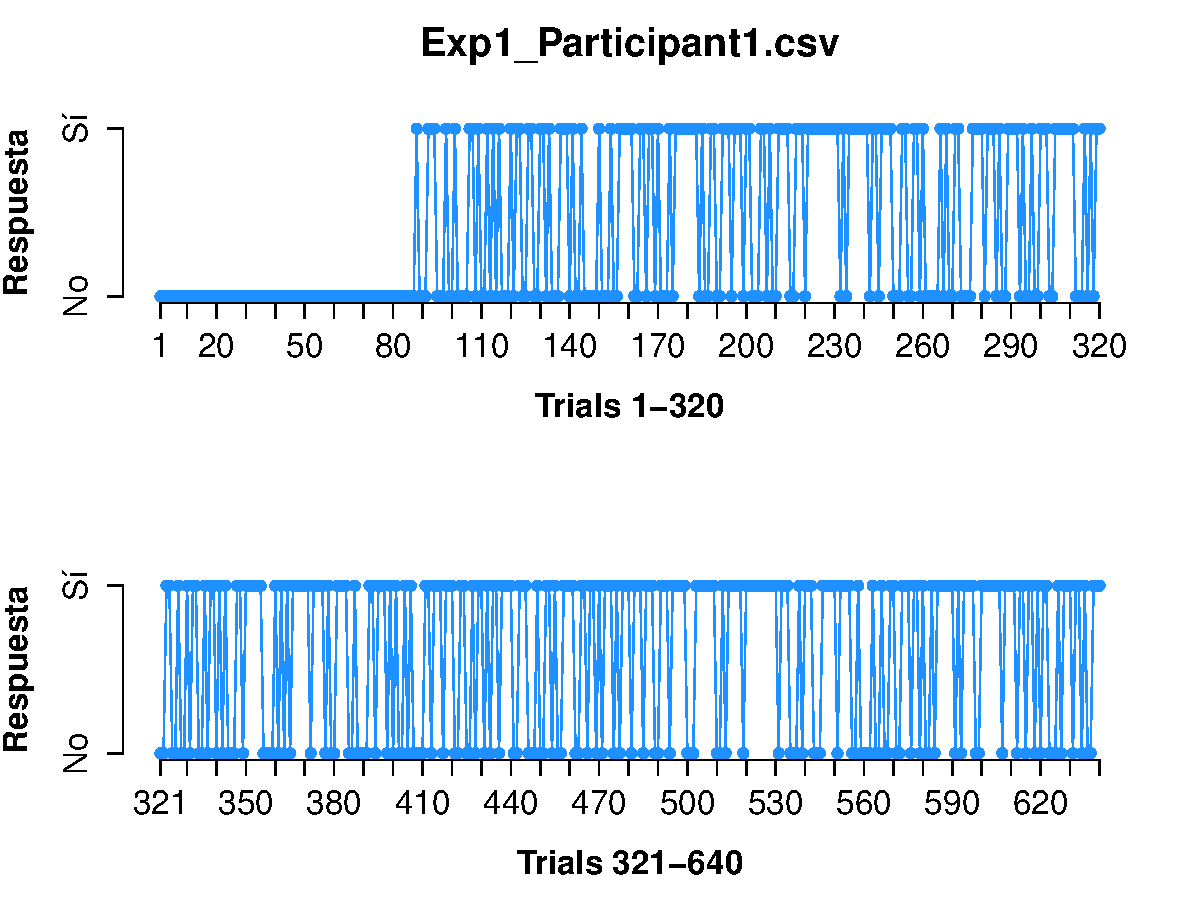
\includegraphics[width=0.30\textwidth]{Figures/Response_Exp1_P1} 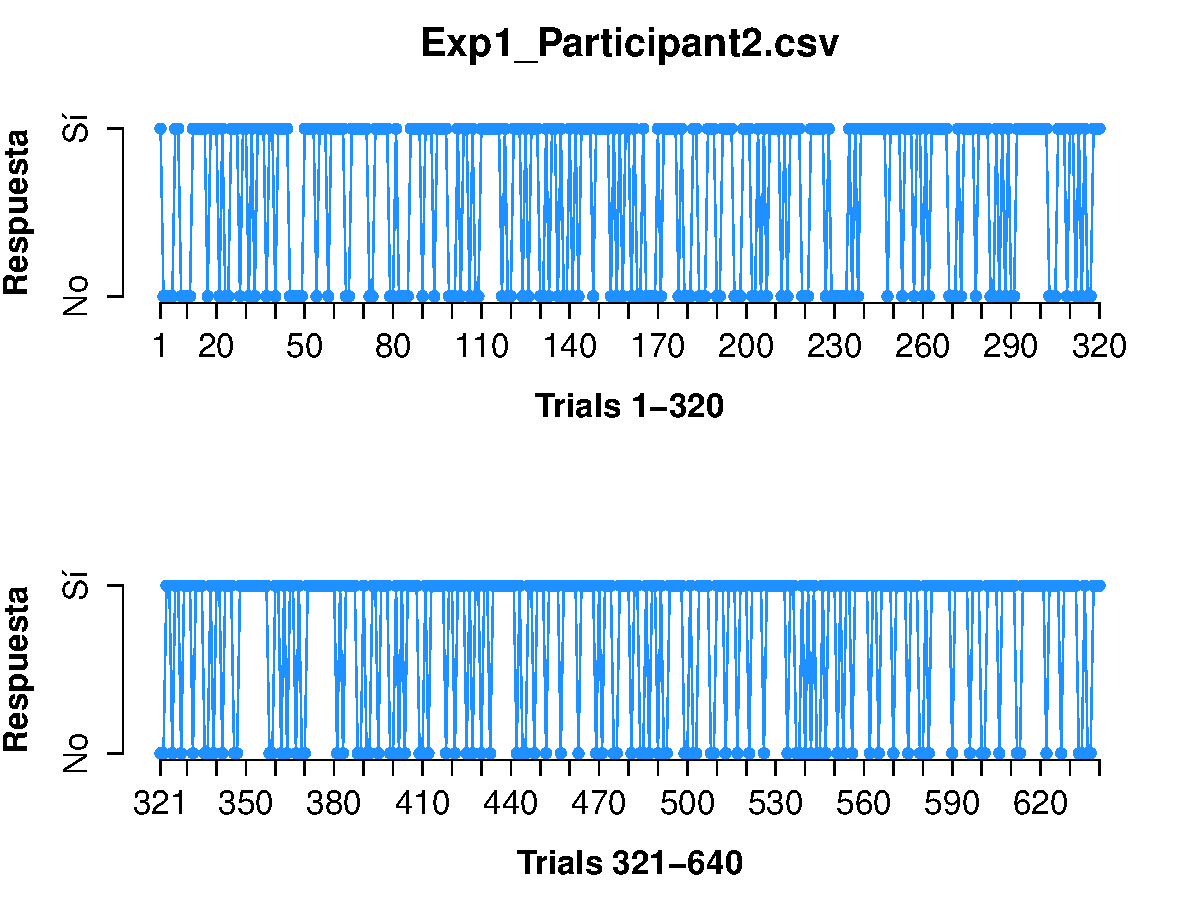
\includegraphics[width=0.30\textwidth]{Figures/Response_Exp1_P2} 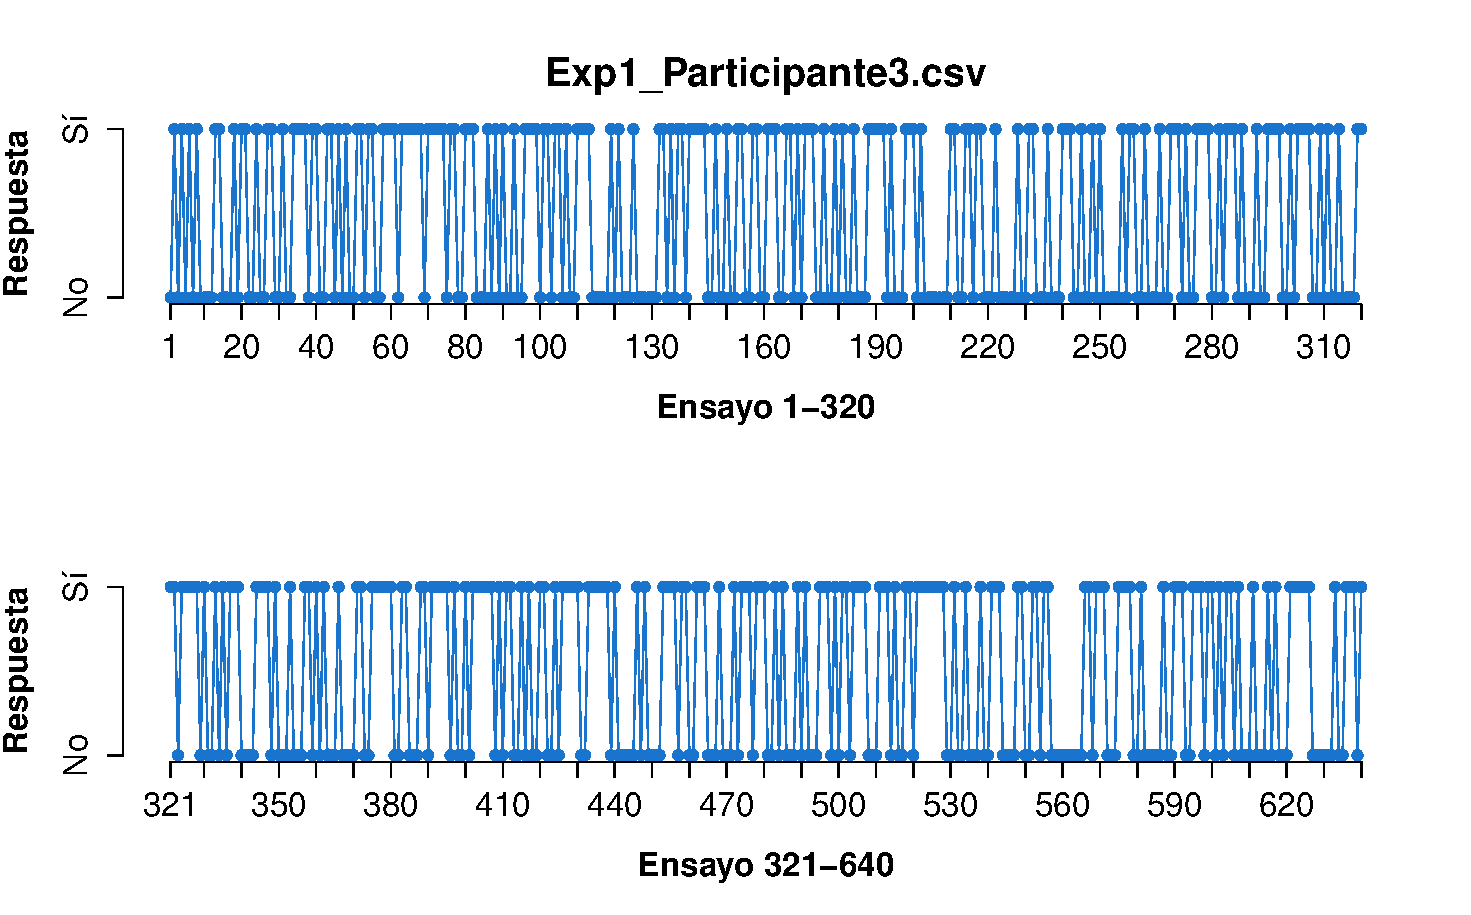
\includegraphics[width=0.30\textwidth]{Figures/Response_Exp1_P3}
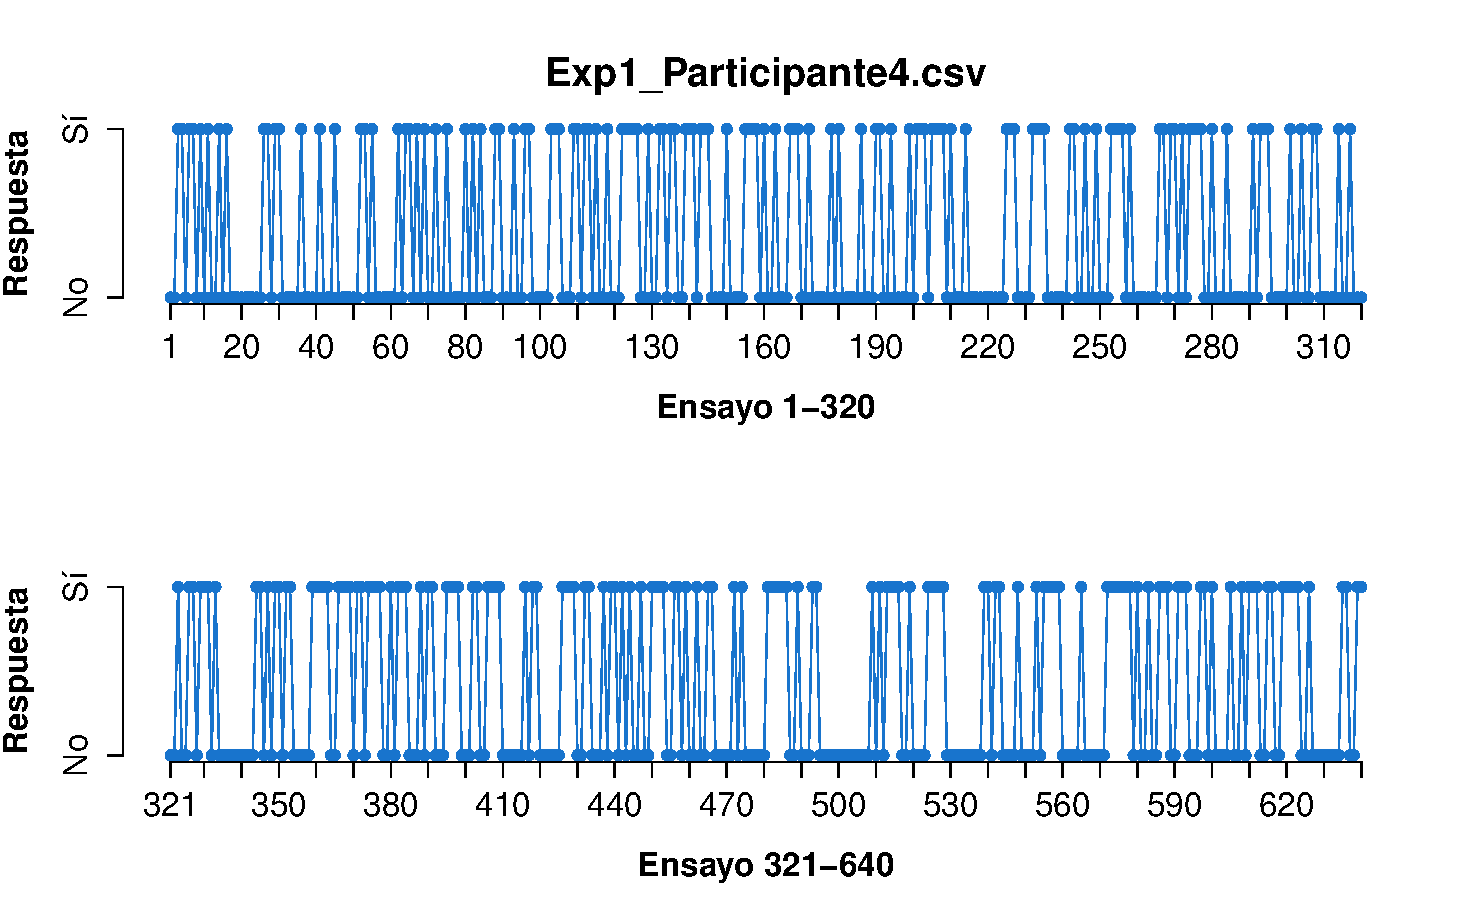
\includegraphics[width=0.30\textwidth]{Figures/Response_Exp1_P4} 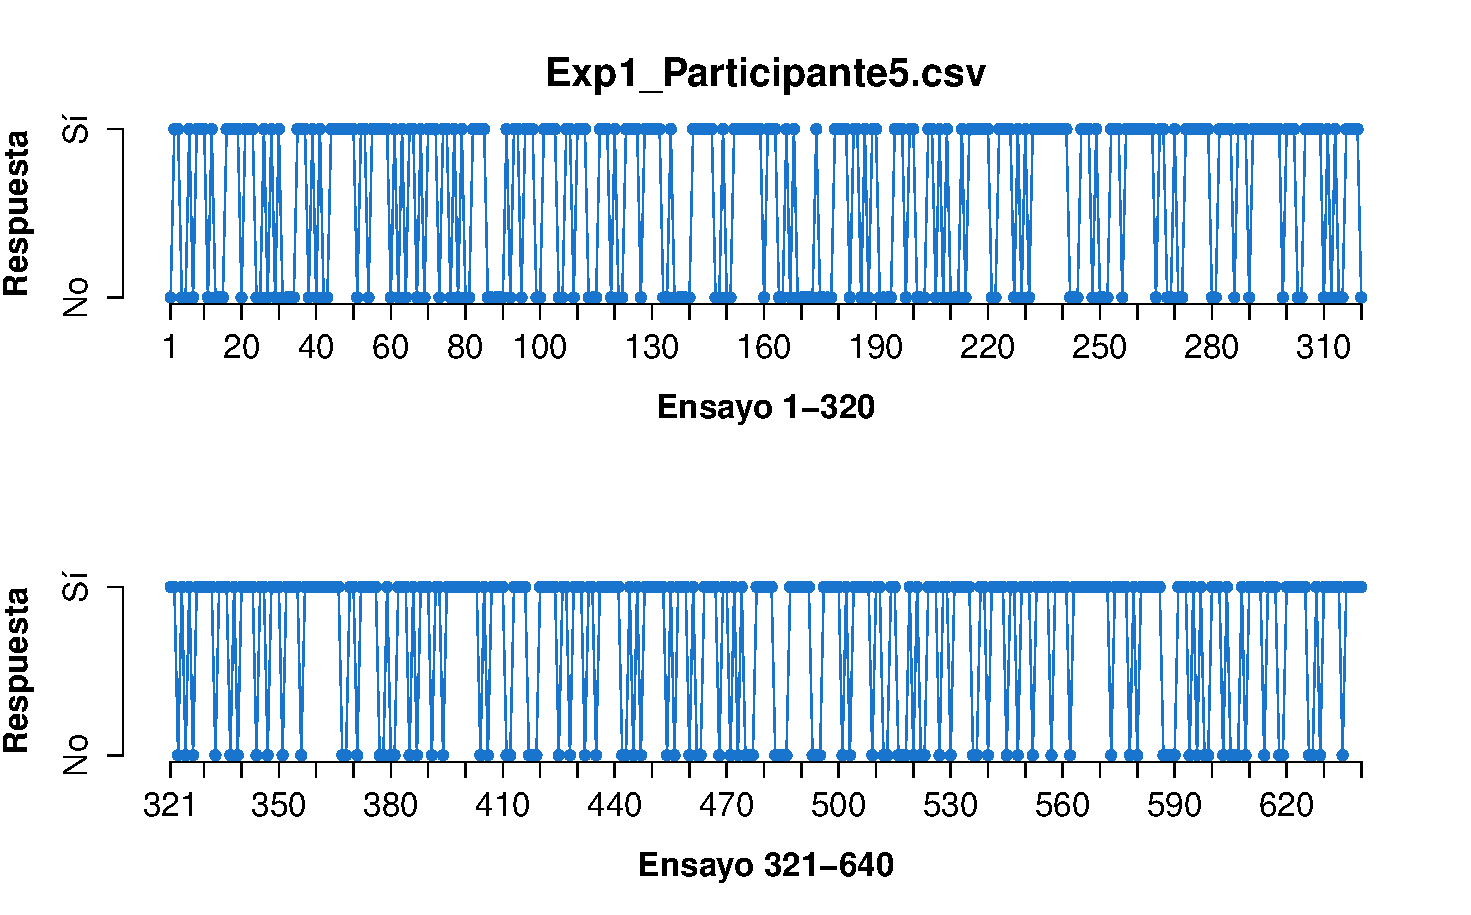
\includegraphics[width=0.30\textwidth]{Figures/Response_Exp1_P5} 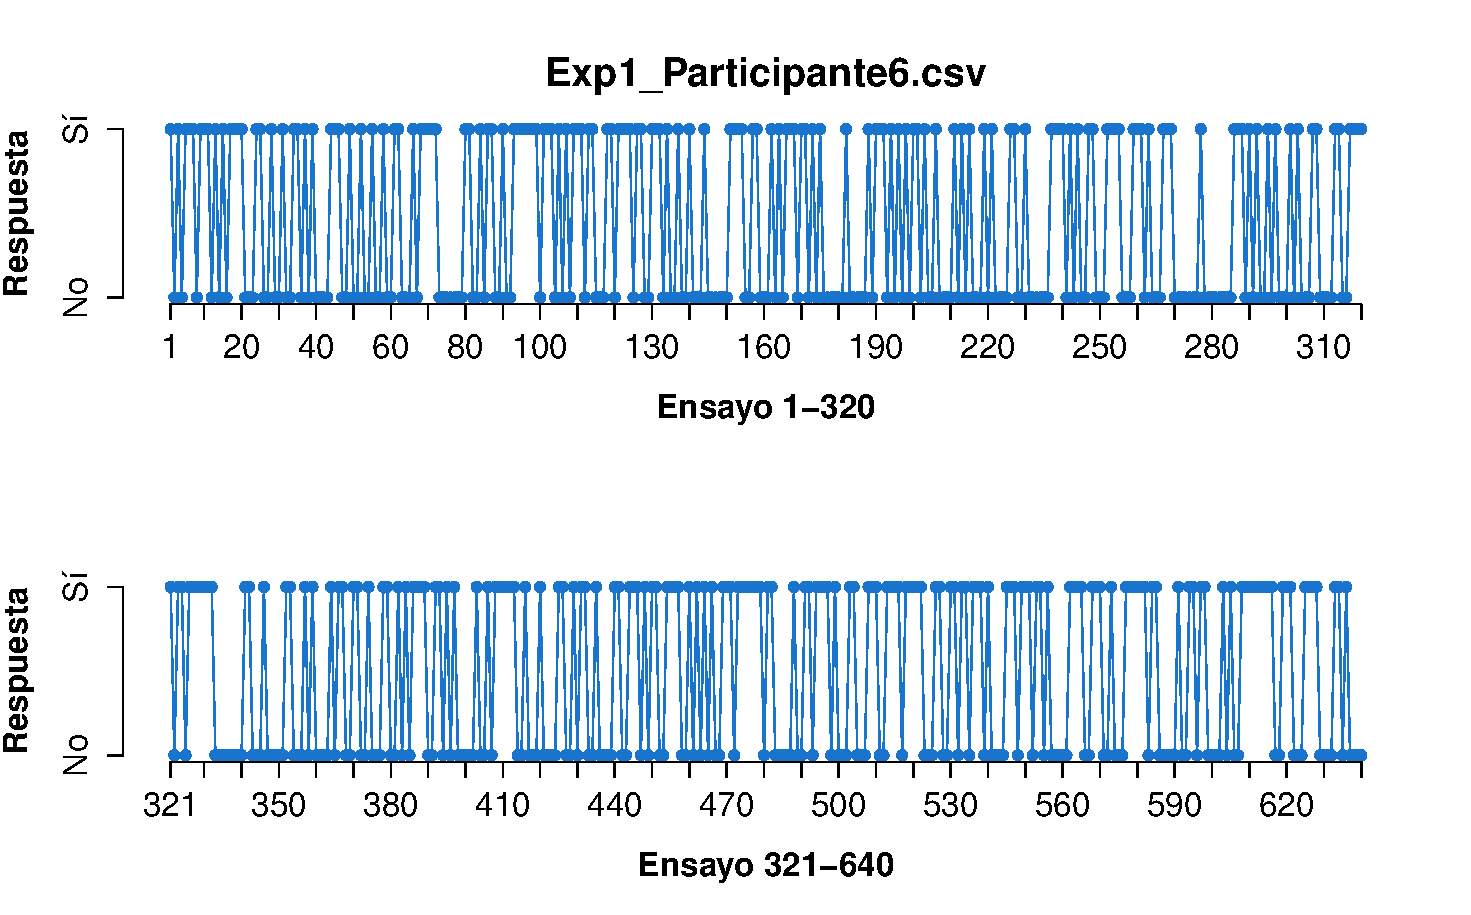
\includegraphics[width=0.30\textwidth]{Figures/Response_Exp1_P6}
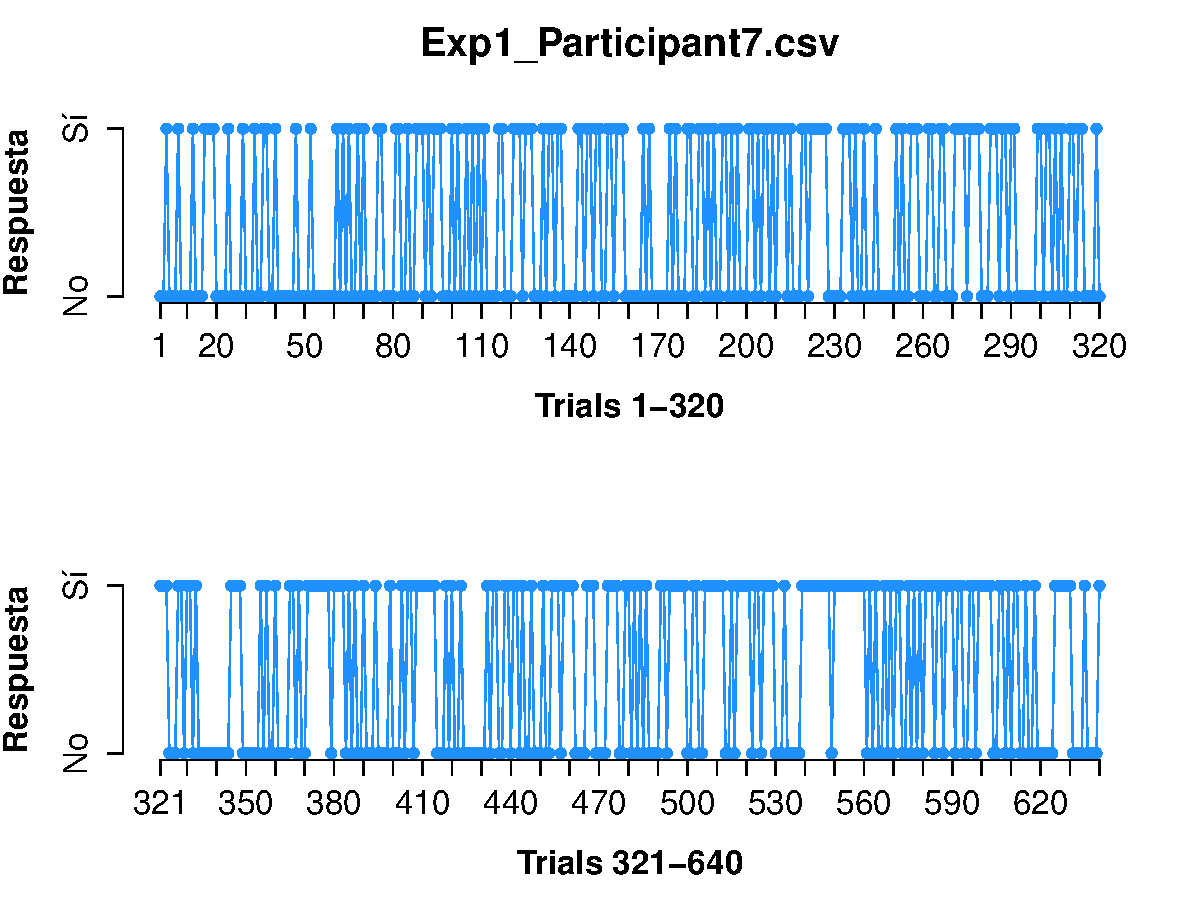
\includegraphics[width=0.30\textwidth]{Figures/Response_Exp1_P7} 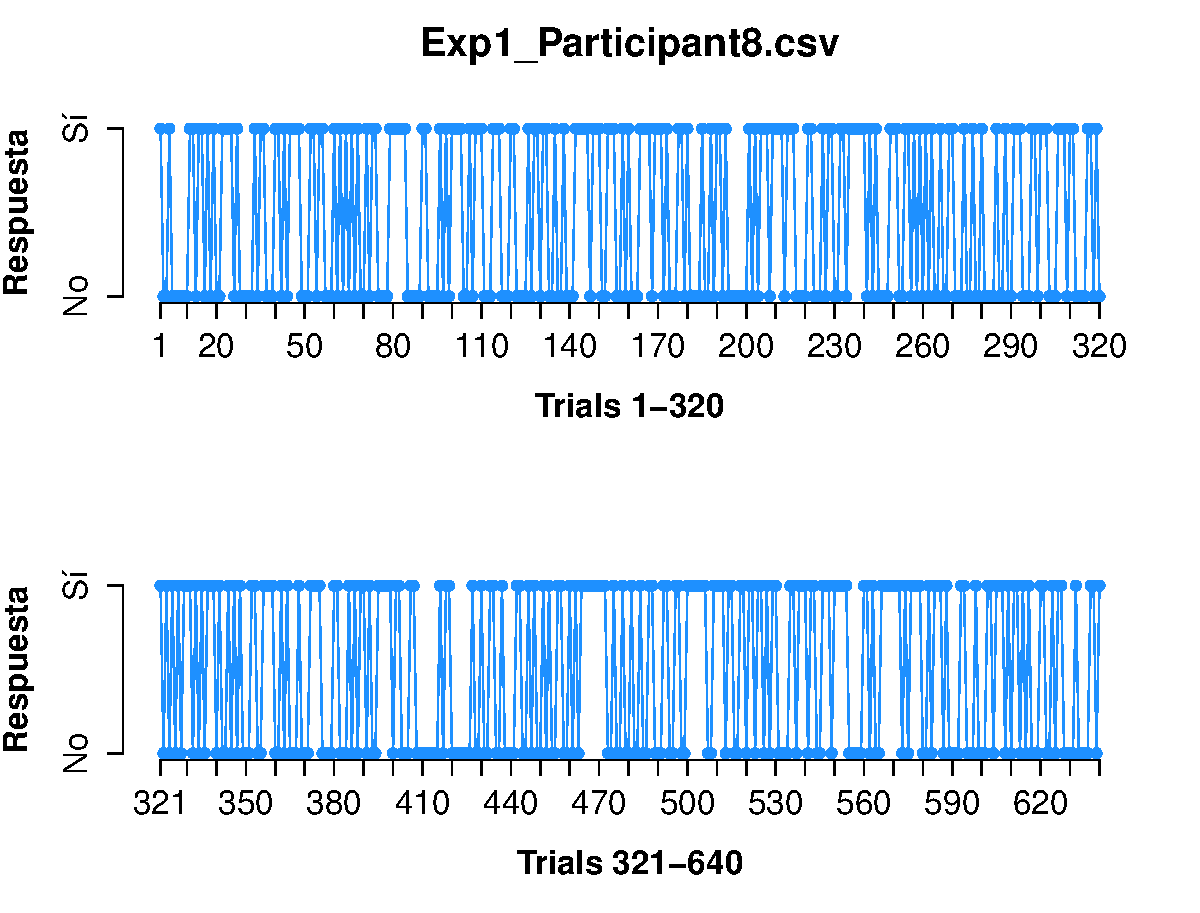
\includegraphics[width=0.30\textwidth]{Figures/Response_Exp1_P8} 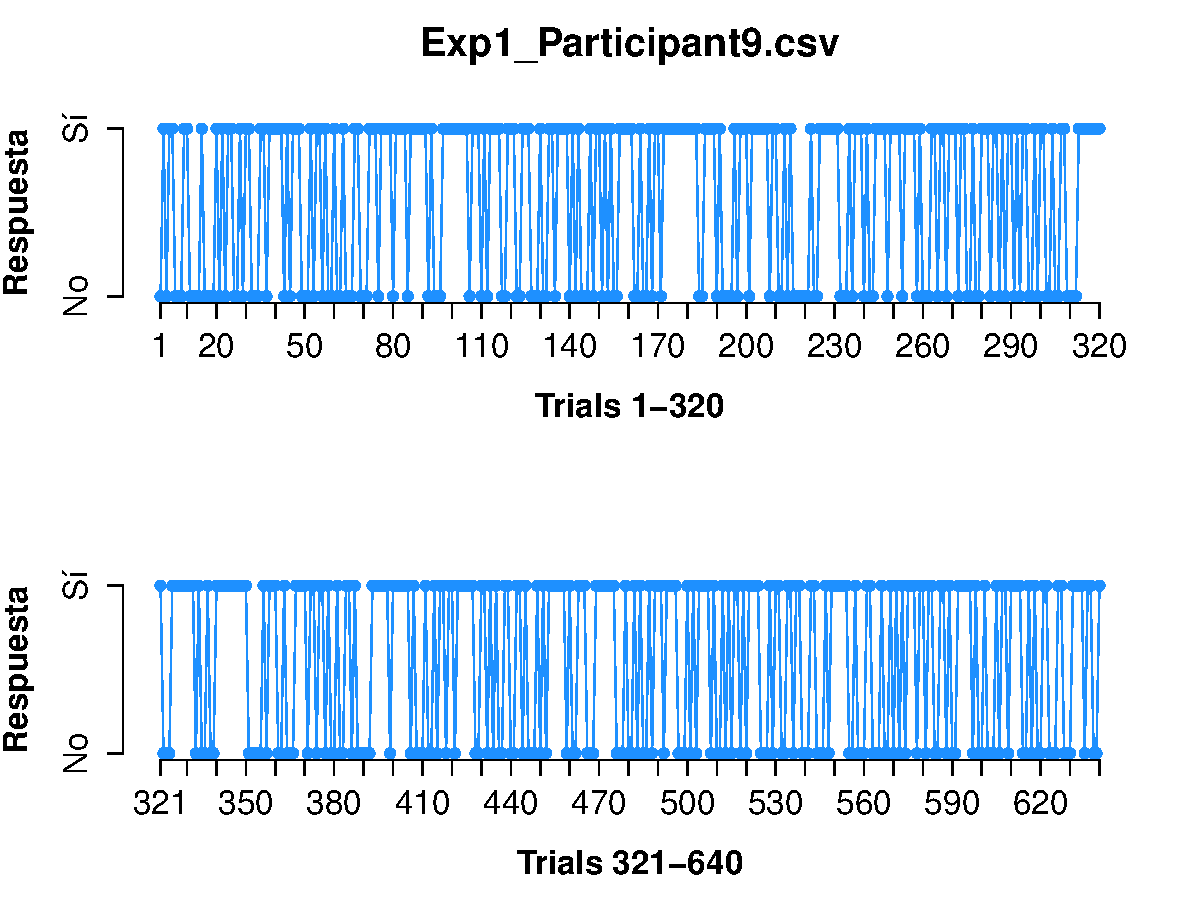
\includegraphics[width=0.30\textwidth]{Figures/Response_Exp1_P9}
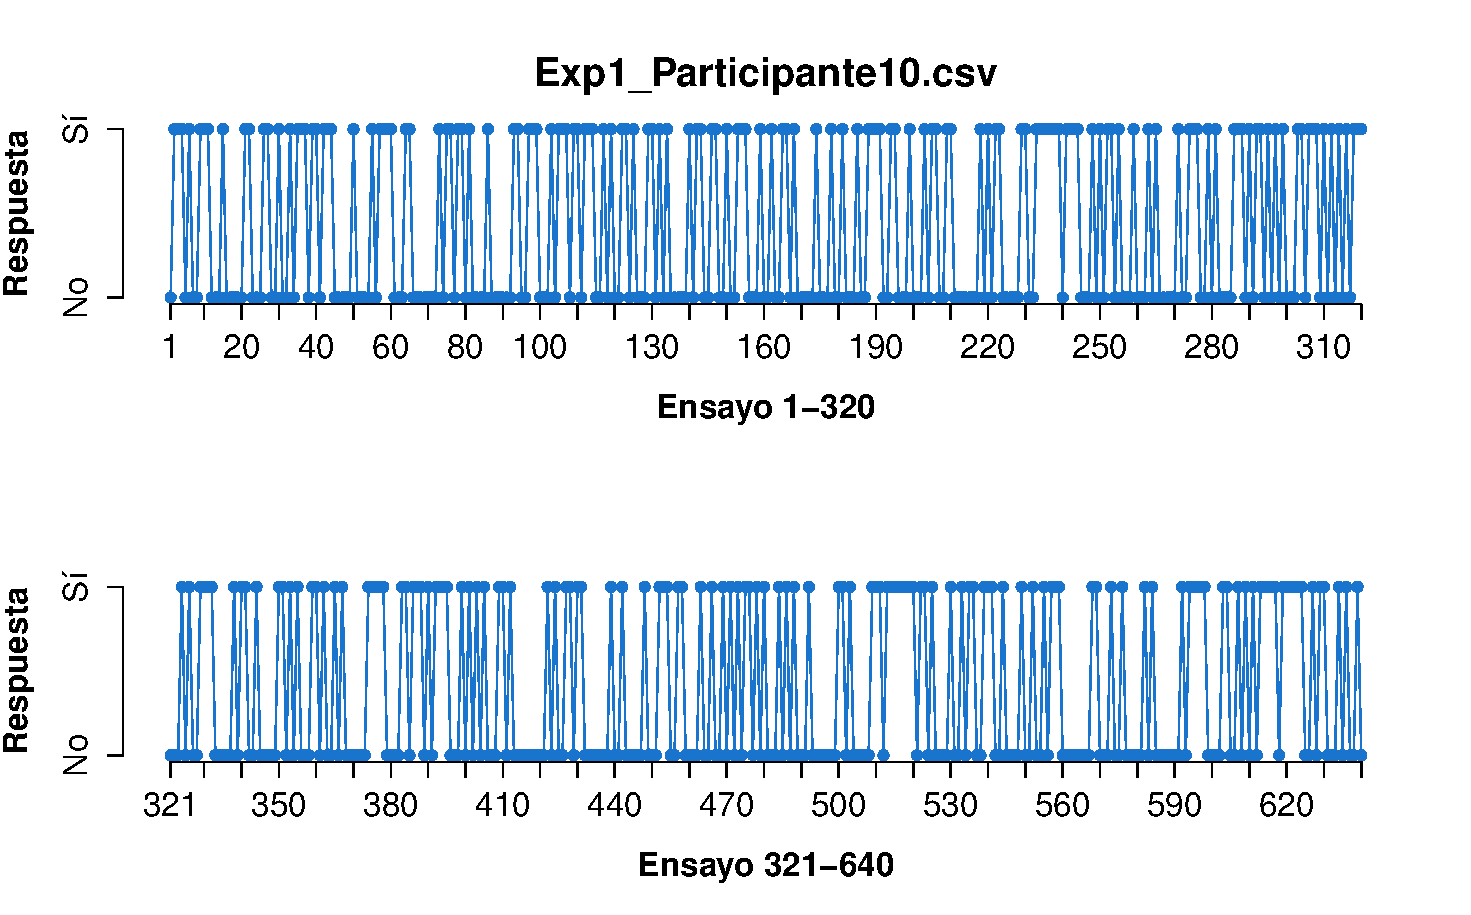
\includegraphics[width=0.30\textwidth]{Figures/Response_Exp1_P10} 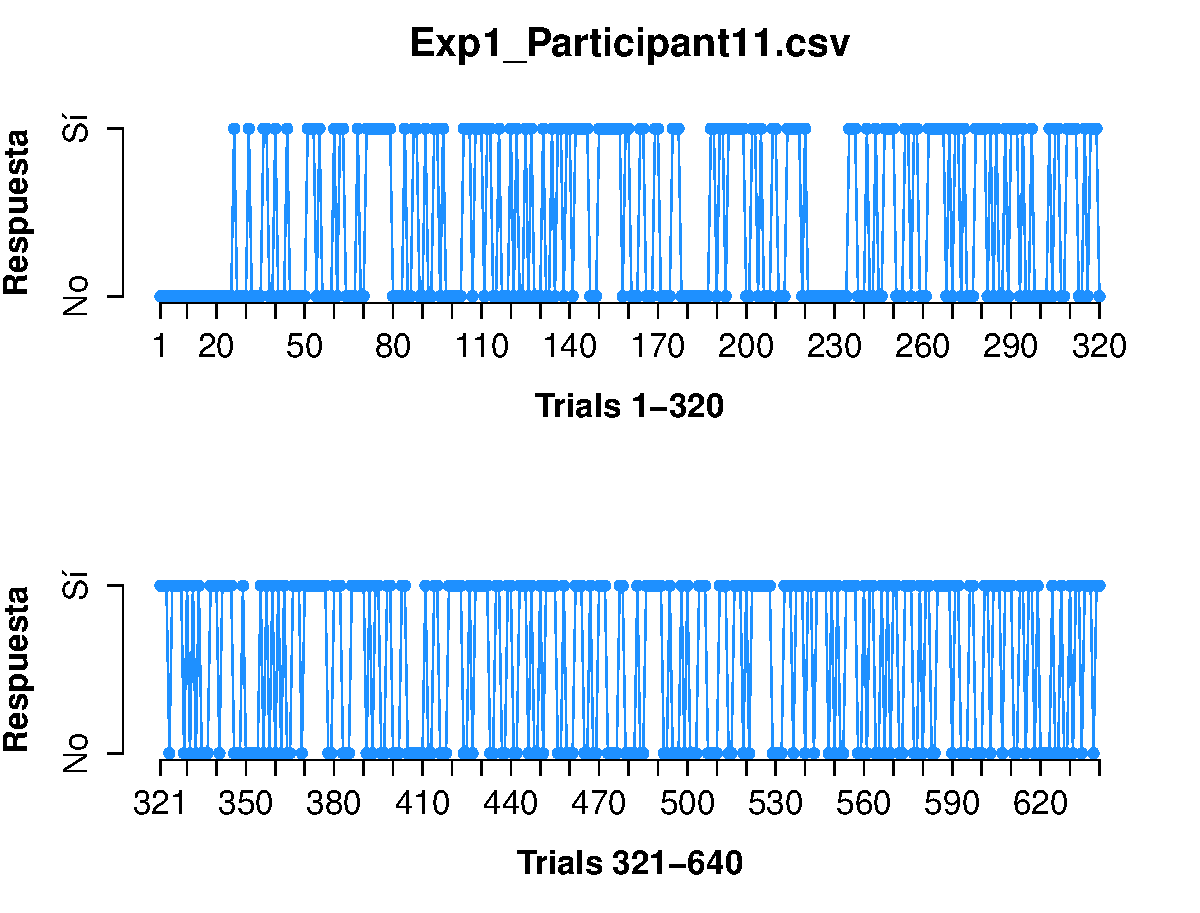
\includegraphics[width=0.30\textwidth]{Figures/Response_Exp1_P11} 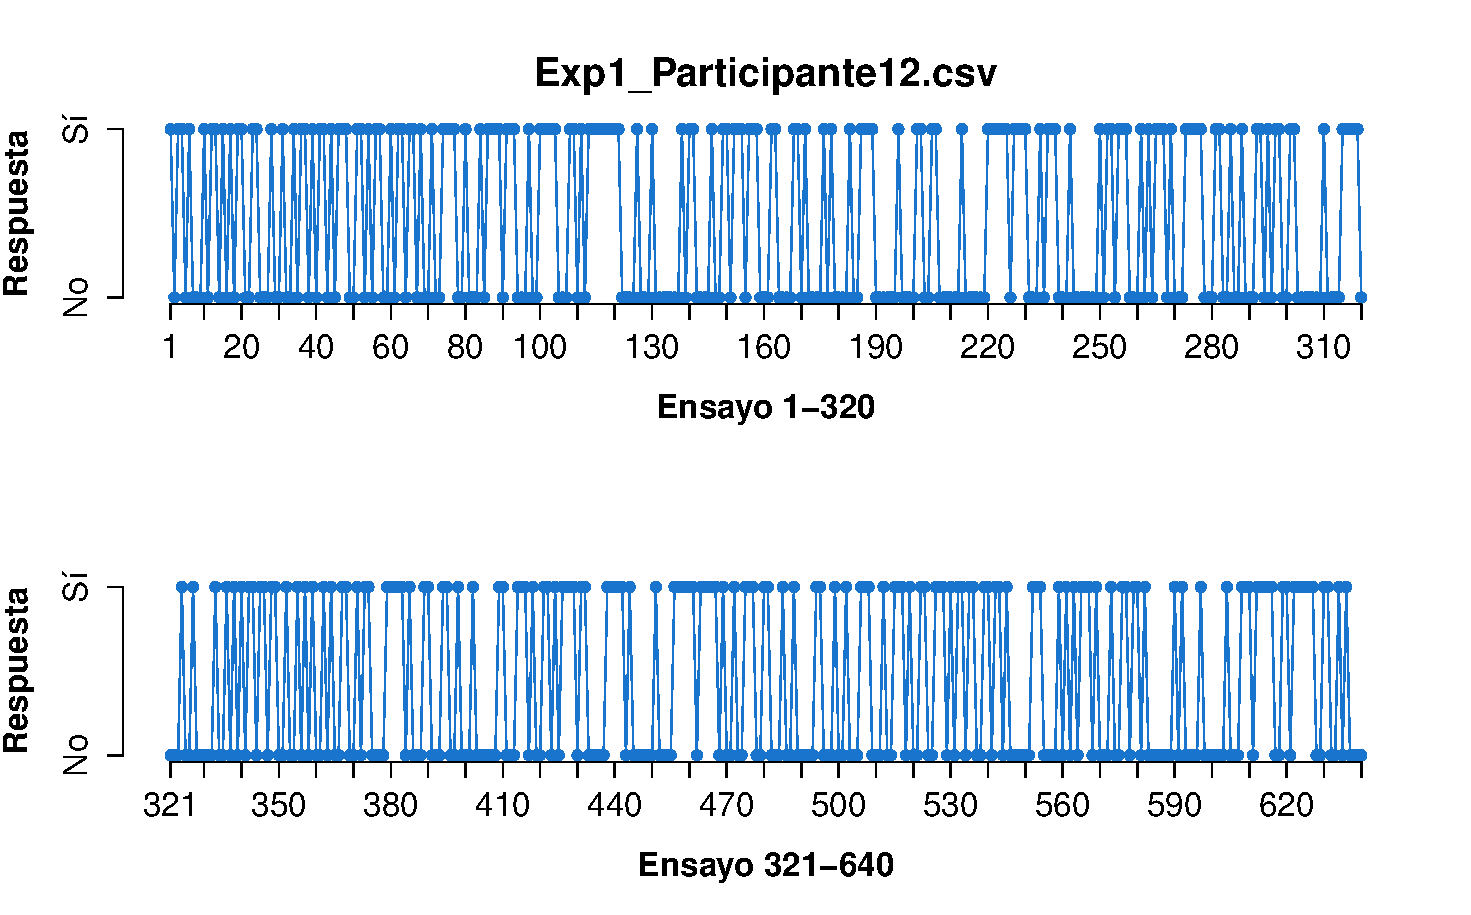
\includegraphics[width=0.30\textwidth]{Figures/Response_Exp1_P12}
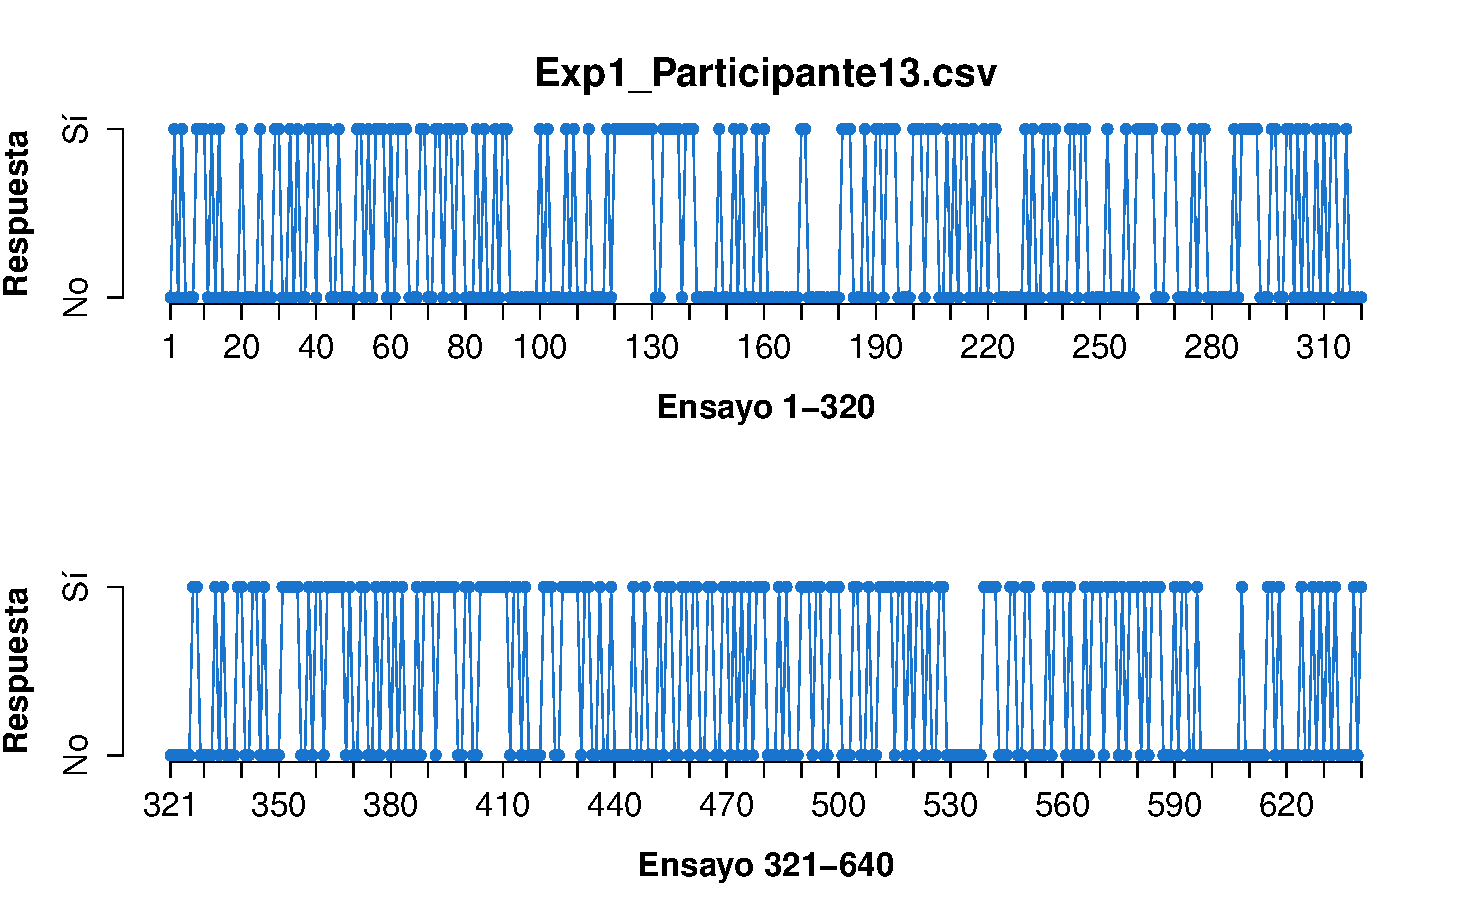
\includegraphics[width=0.30\textwidth]{Figures/Response_Exp1_P13} 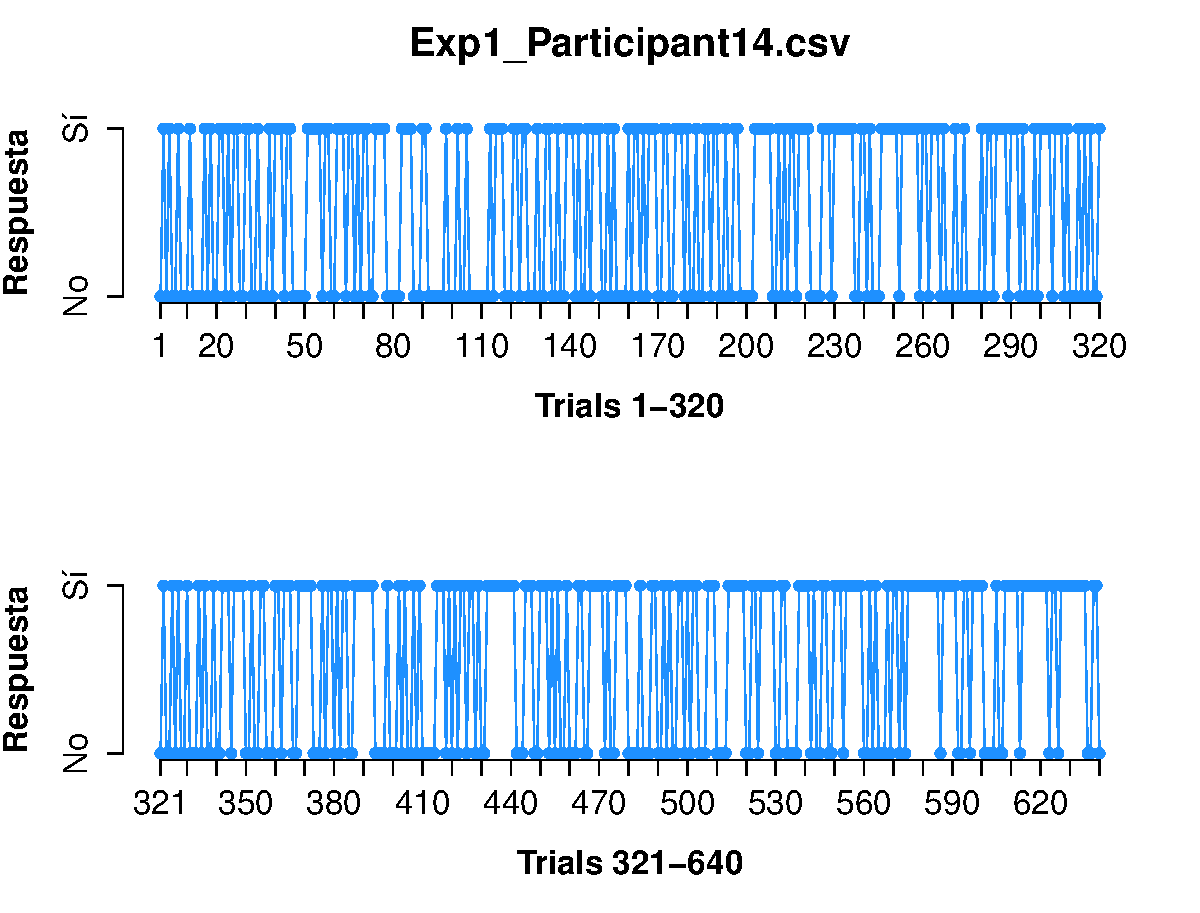
\includegraphics[width=0.30\textwidth]{Figures/Response_Exp1_P14} 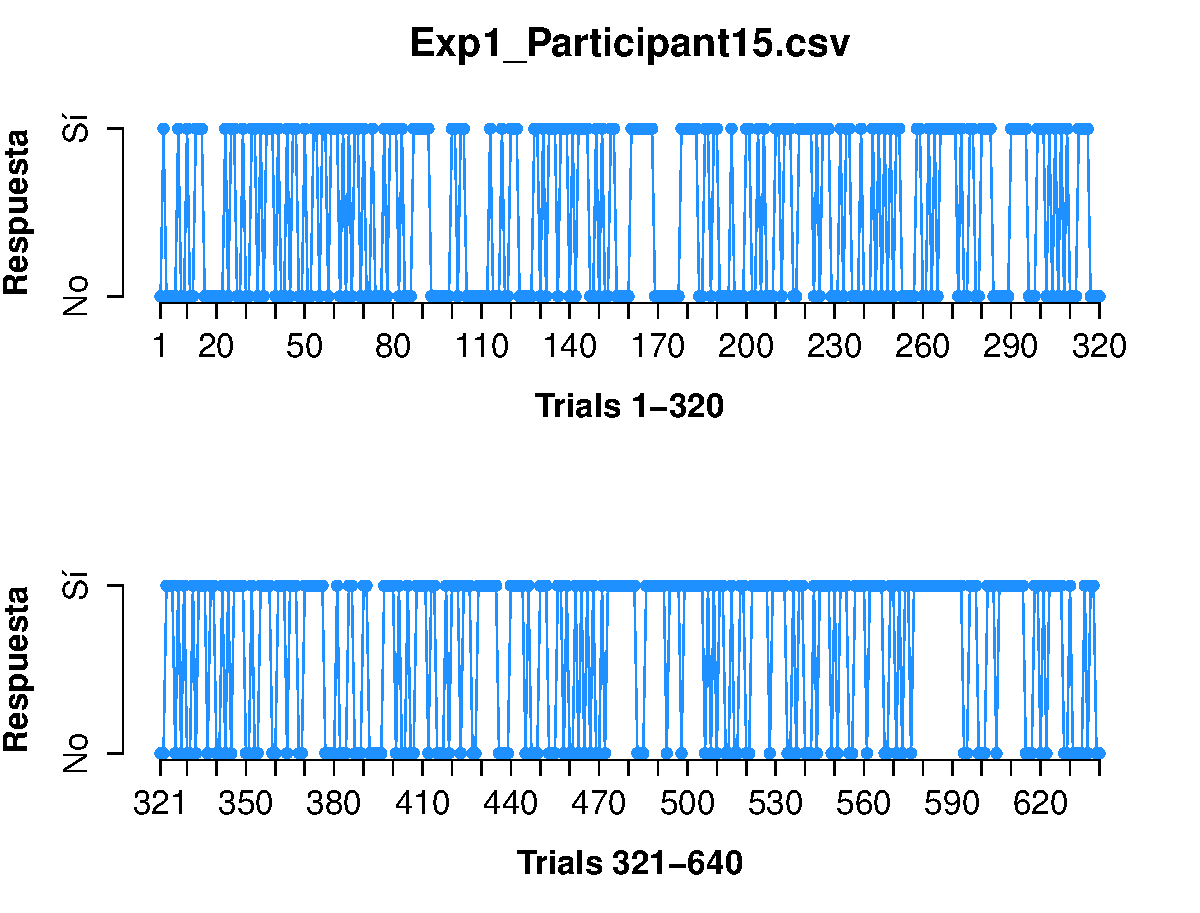
\includegraphics[width=0.30\textwidth]{Figures/Response_Exp1_P15}
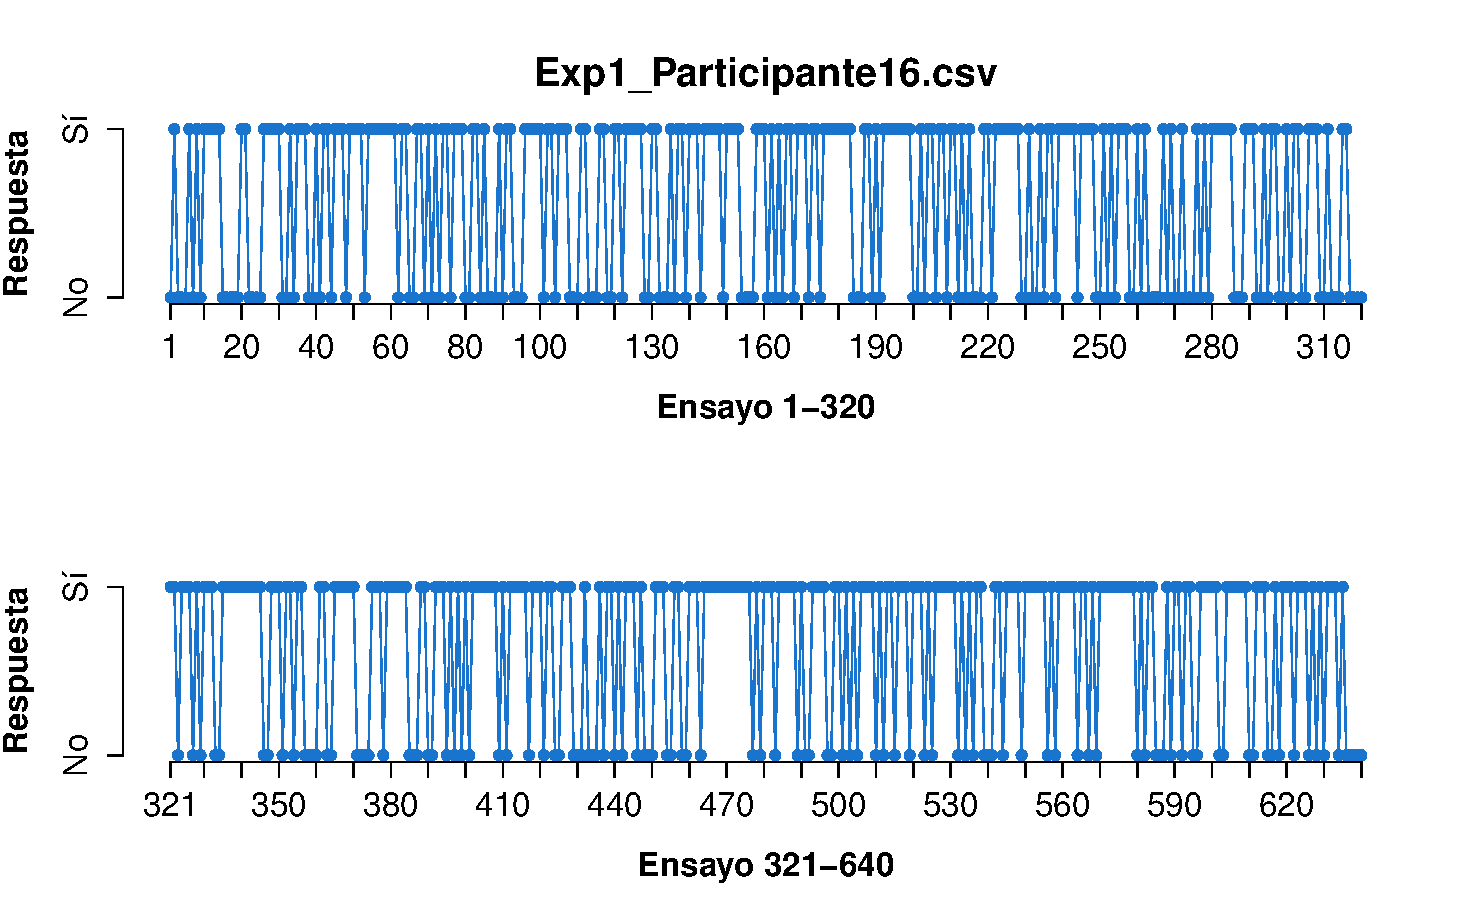
\includegraphics[width=0.30\textwidth]{Figures/Response_Exp1_P16} 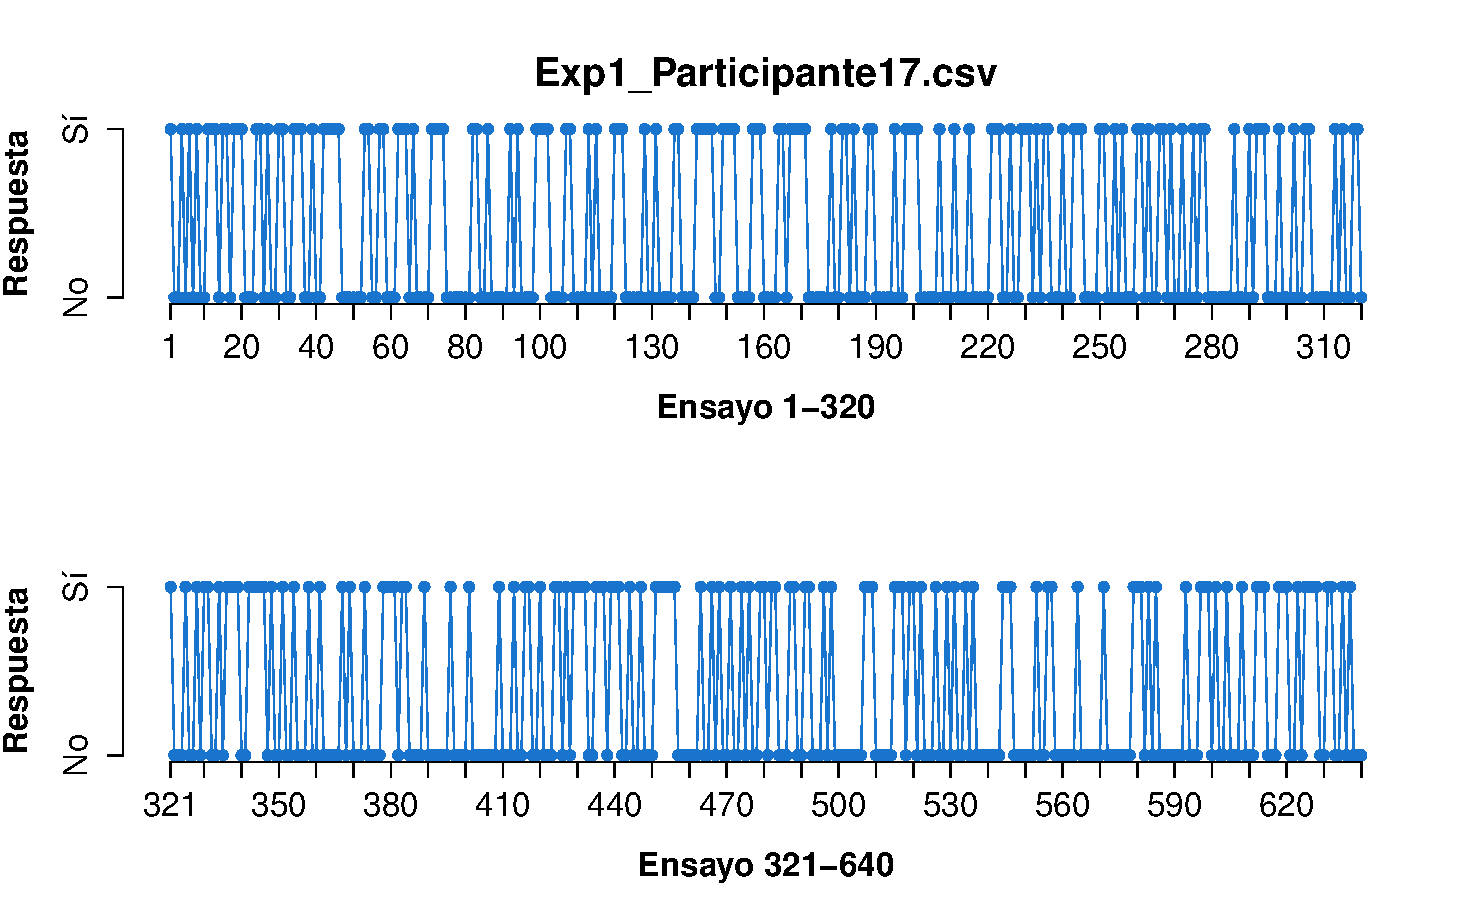
\includegraphics[width=0.30\textwidth]{Figures/Response_Exp1_P17} 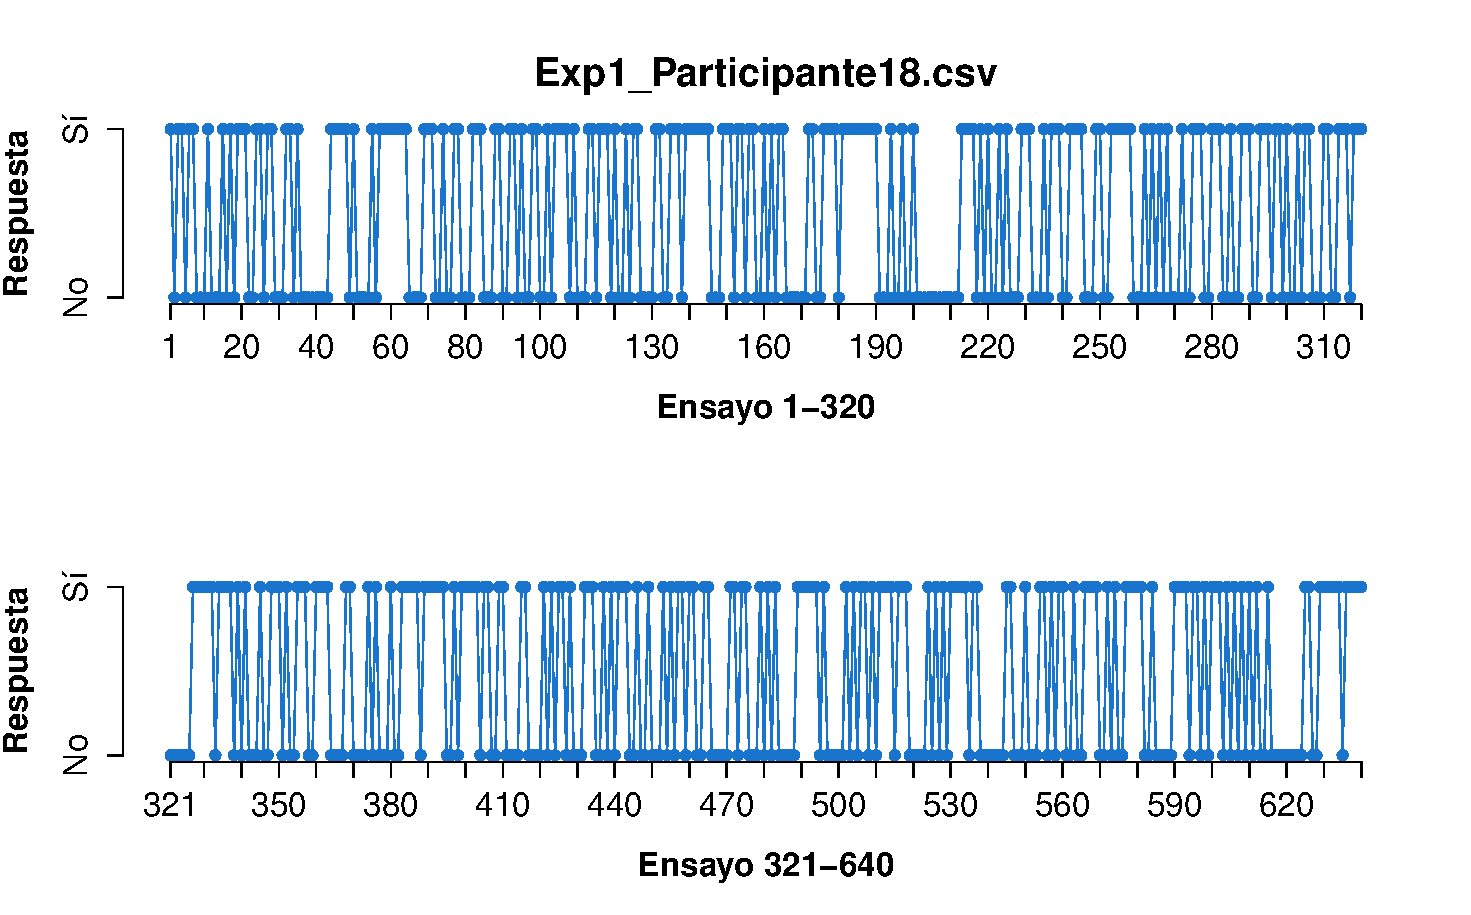
\includegraphics[width=0.30\textwidth]{Figures/Response_Exp1_P18}
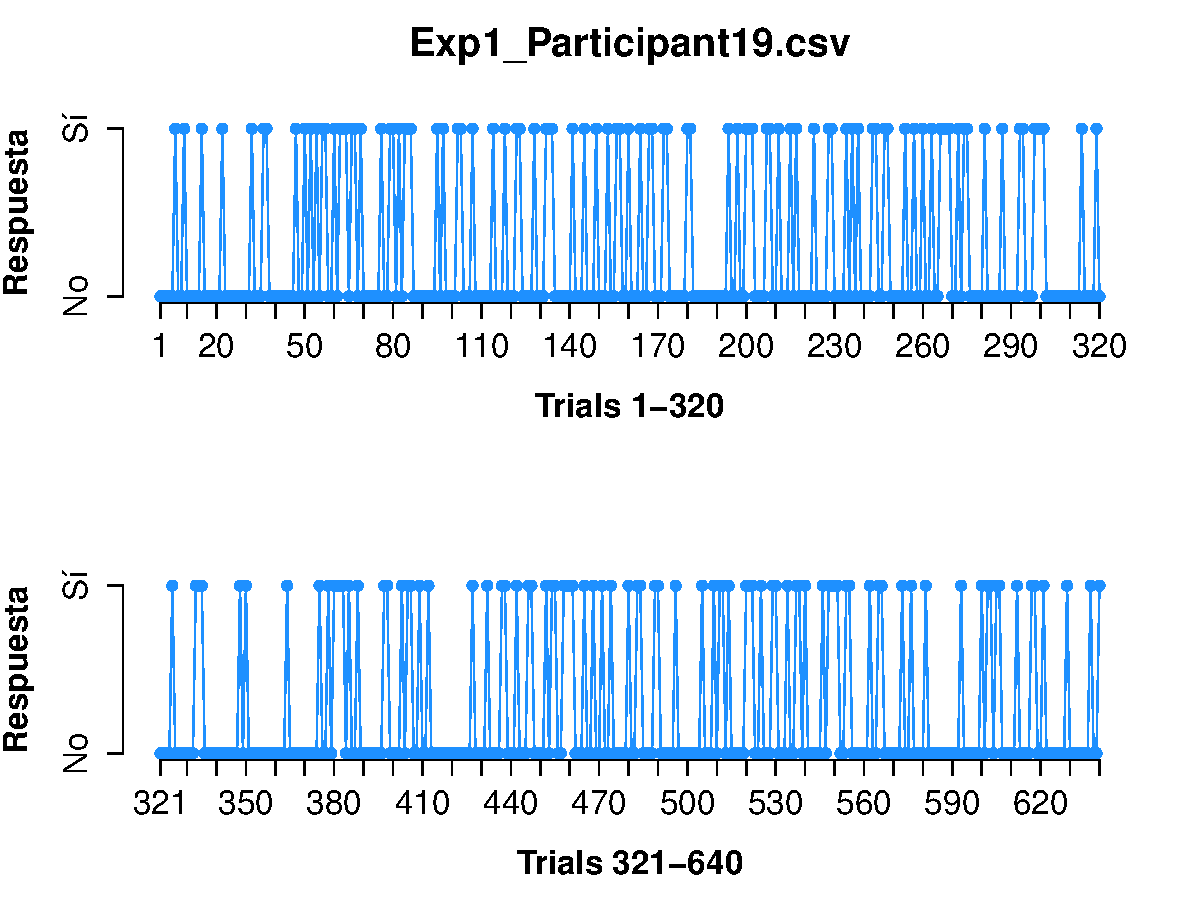
\includegraphics[width=0.30\textwidth]{Figures/Response_Exp1_P19} 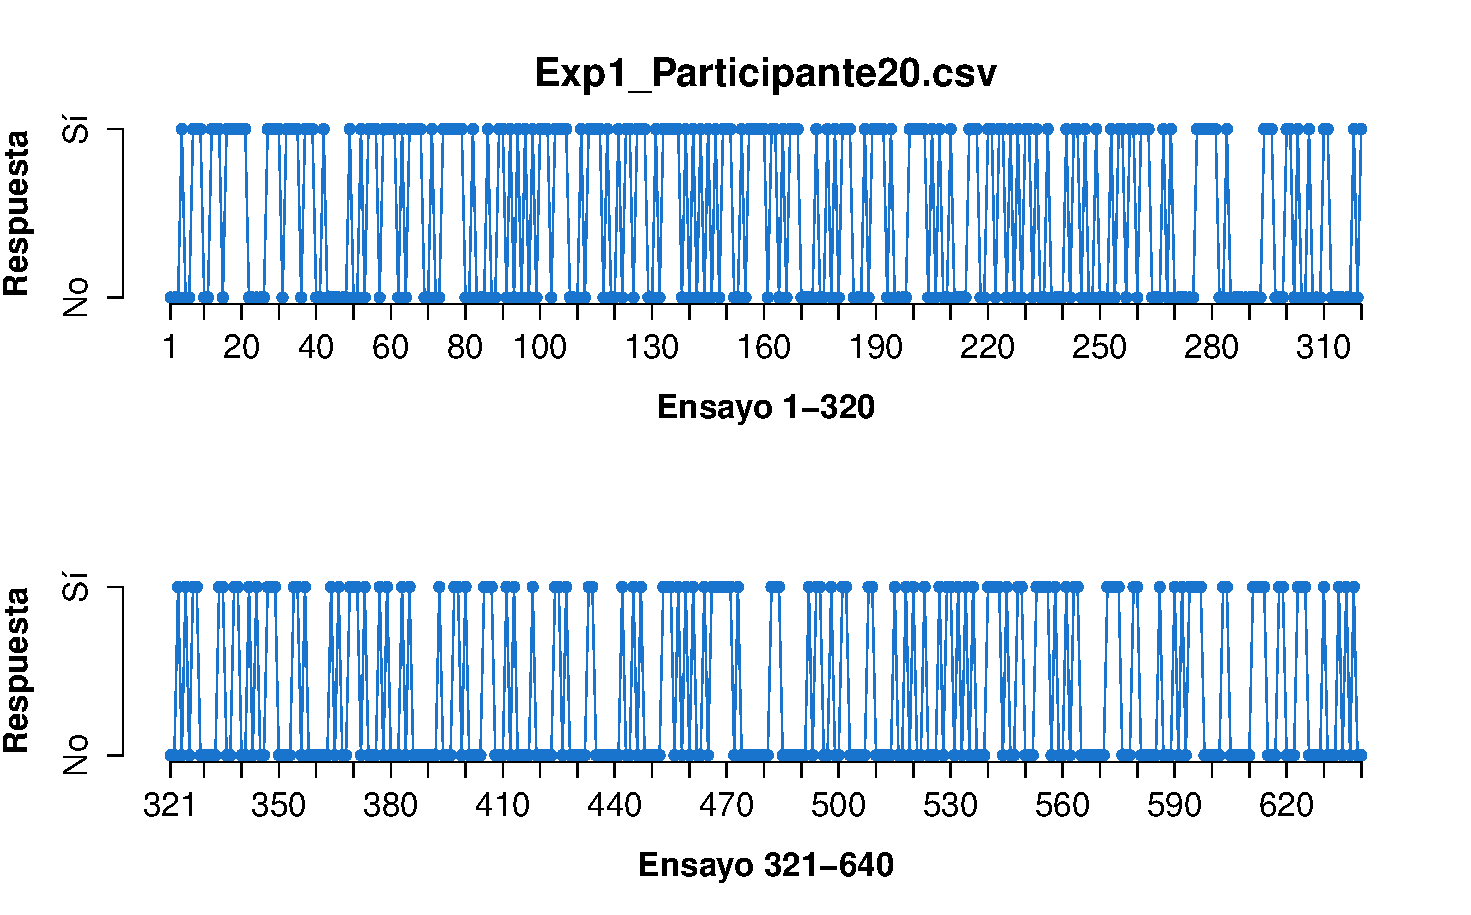
\includegraphics[width=0.30\textwidth]{Figures/Response_Exp1_P20} 
%\decoRule
\caption[Respuesta binaria registrada ensayo a ensayo; Experimento 1]{Respuestas registradas en cada ensayo por los veinte participantes del Experimento 1, para la tarea de detección binaria. Por cada participante se incluyen dos gráficas que presentan las respuestas emitidas en la primera y la segunda mitad del experimento, (panel superior e inferior, respectivamente).}
\label{fig:Response_E1}
\end{figure}

\begin{figure}[th]
\centering
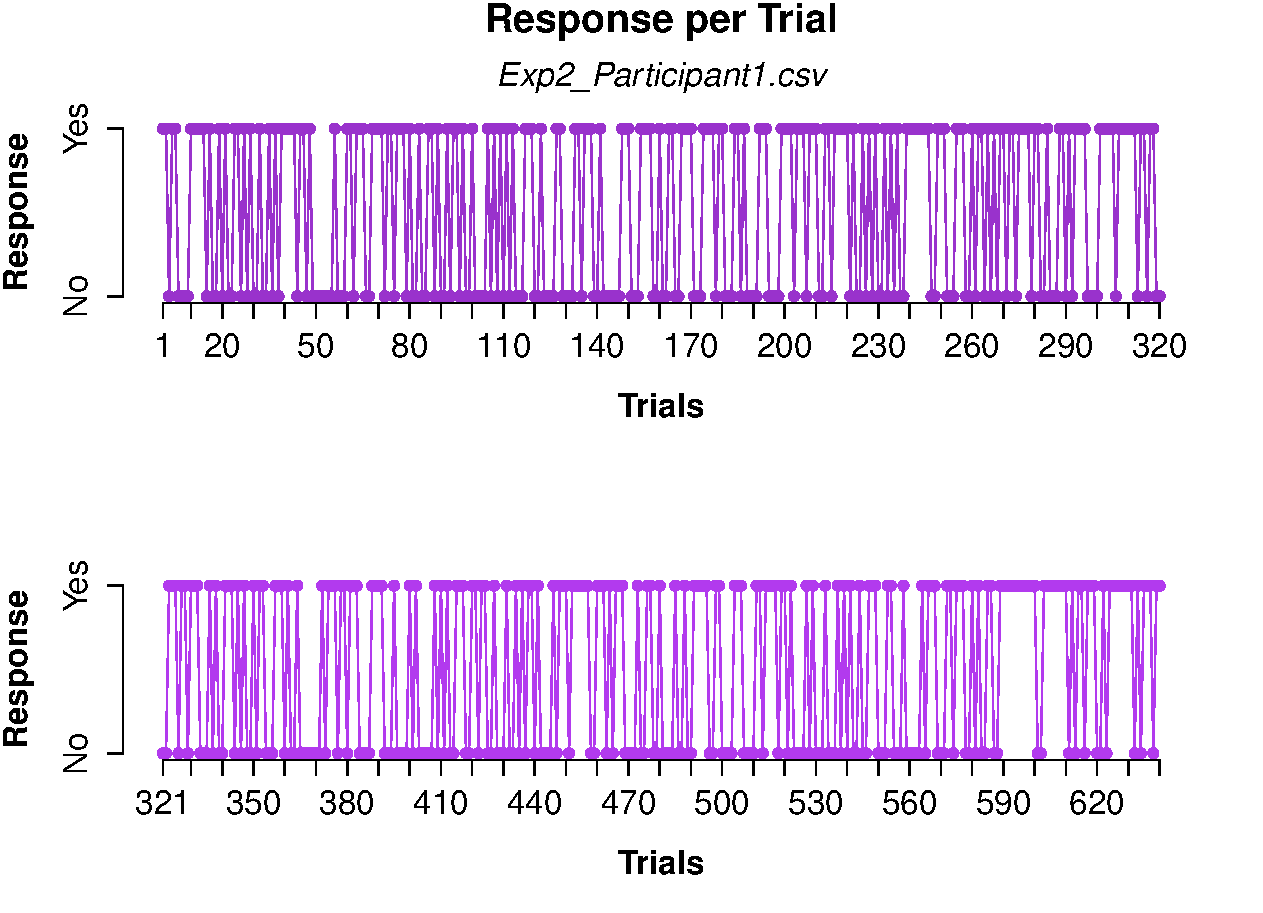
\includegraphics[width=0.30\textwidth]{Figures/Response_Exp2_P1} 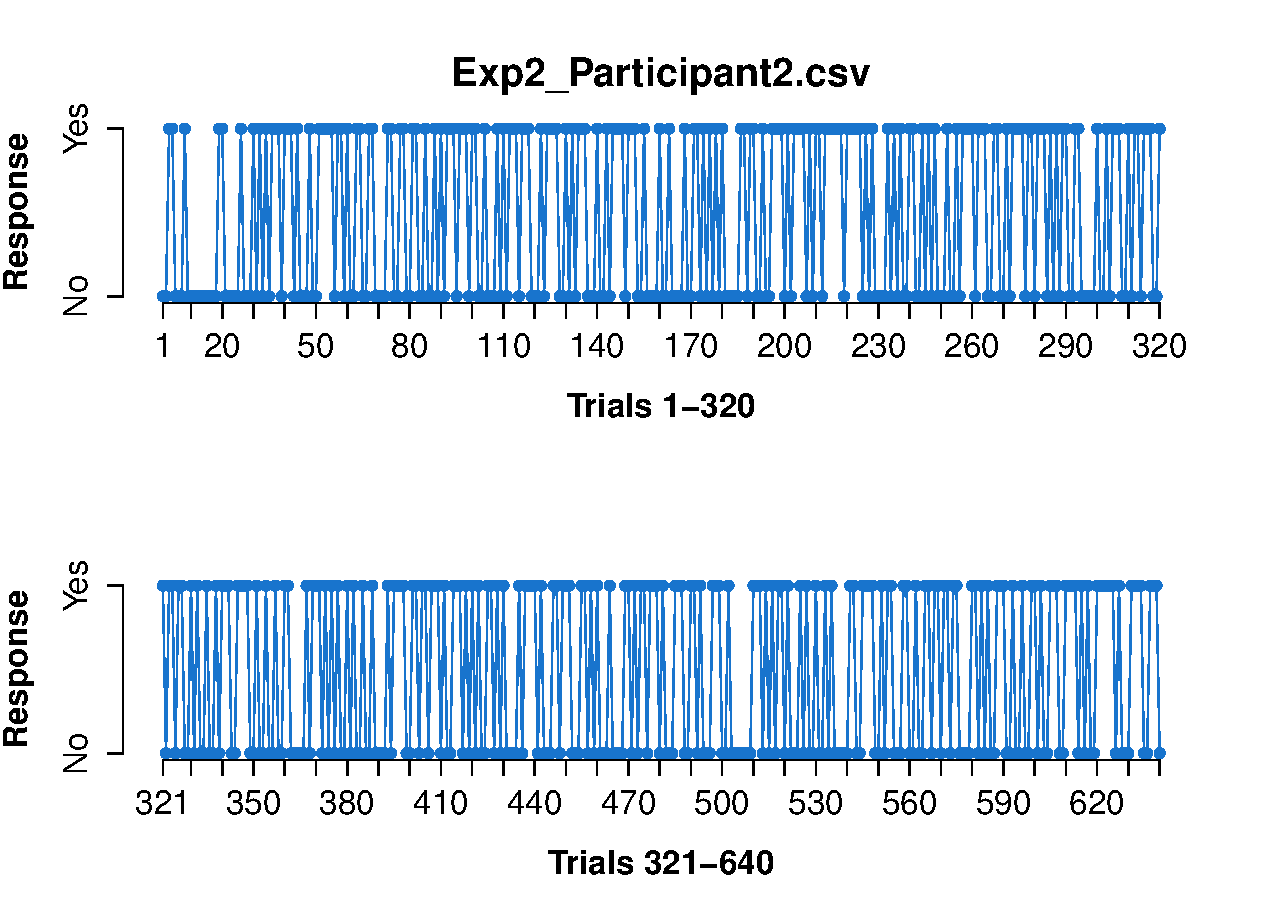
\includegraphics[width=0.30\textwidth]{Figures/Response_Exp2_P2} 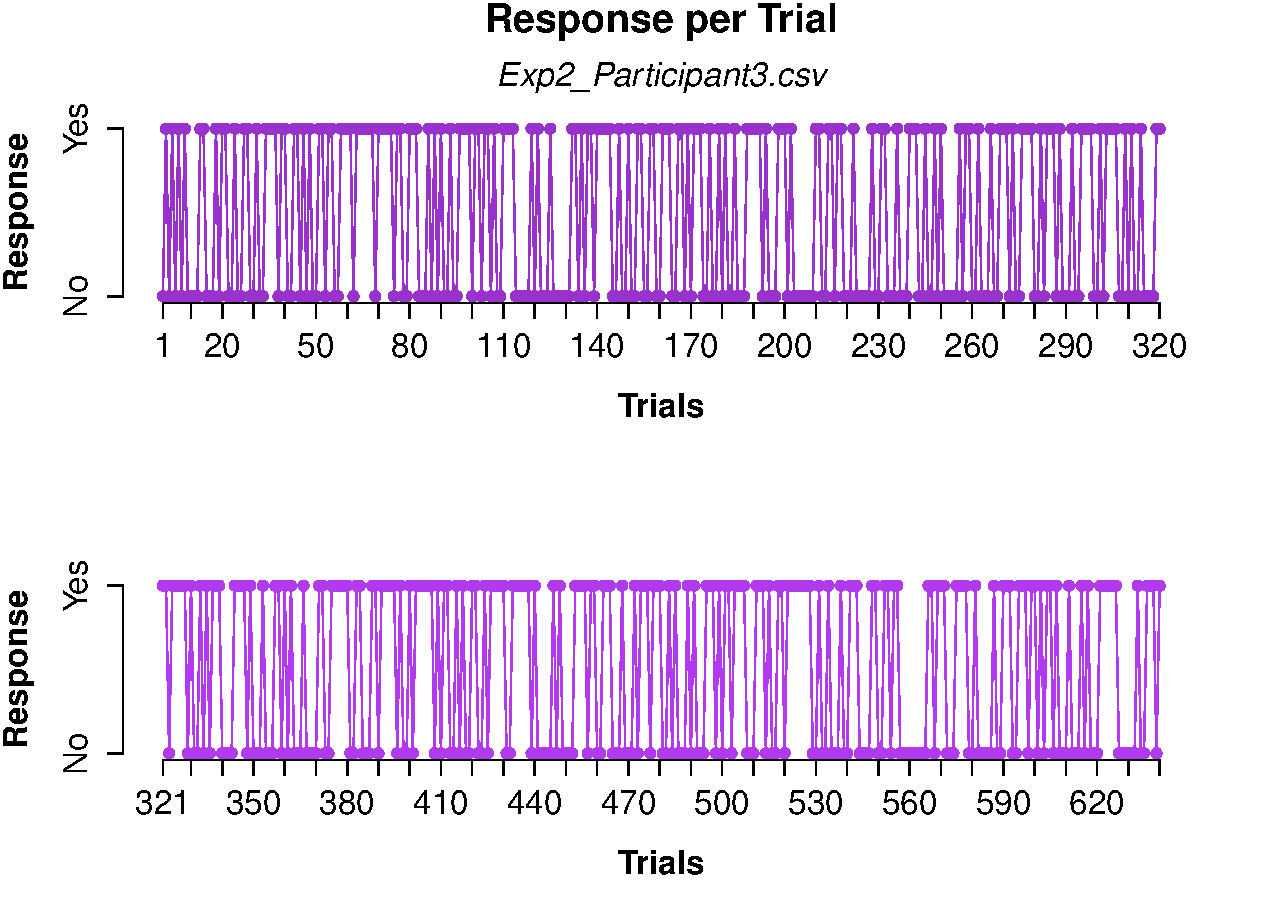
\includegraphics[width=0.30\textwidth]{Figures/Response_Exp2_P3}
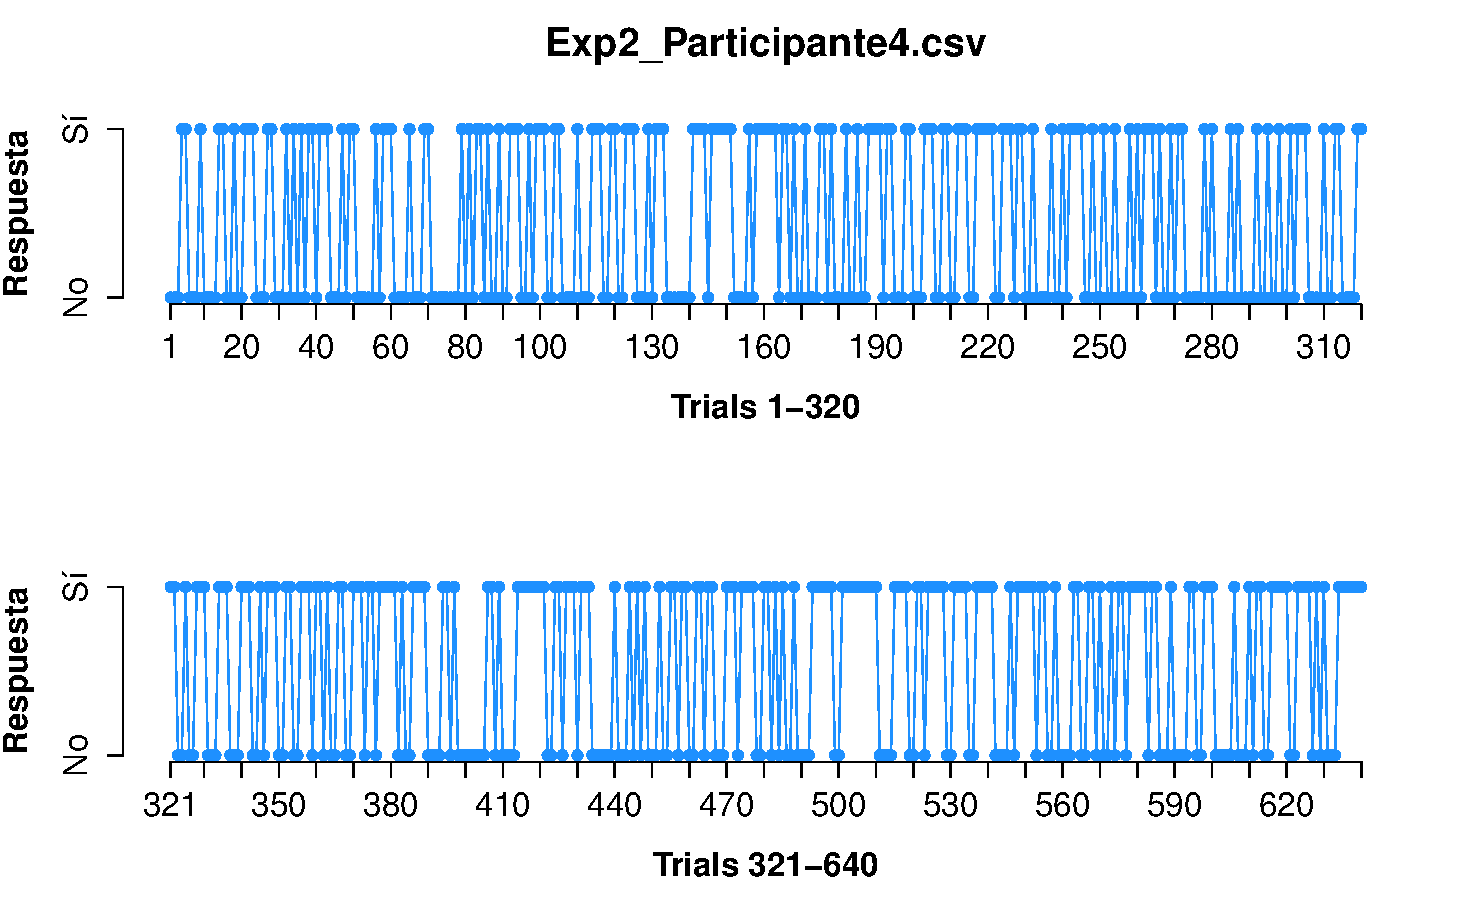
\includegraphics[width=0.30\textwidth]{Figures/Response_Exp2_P4} 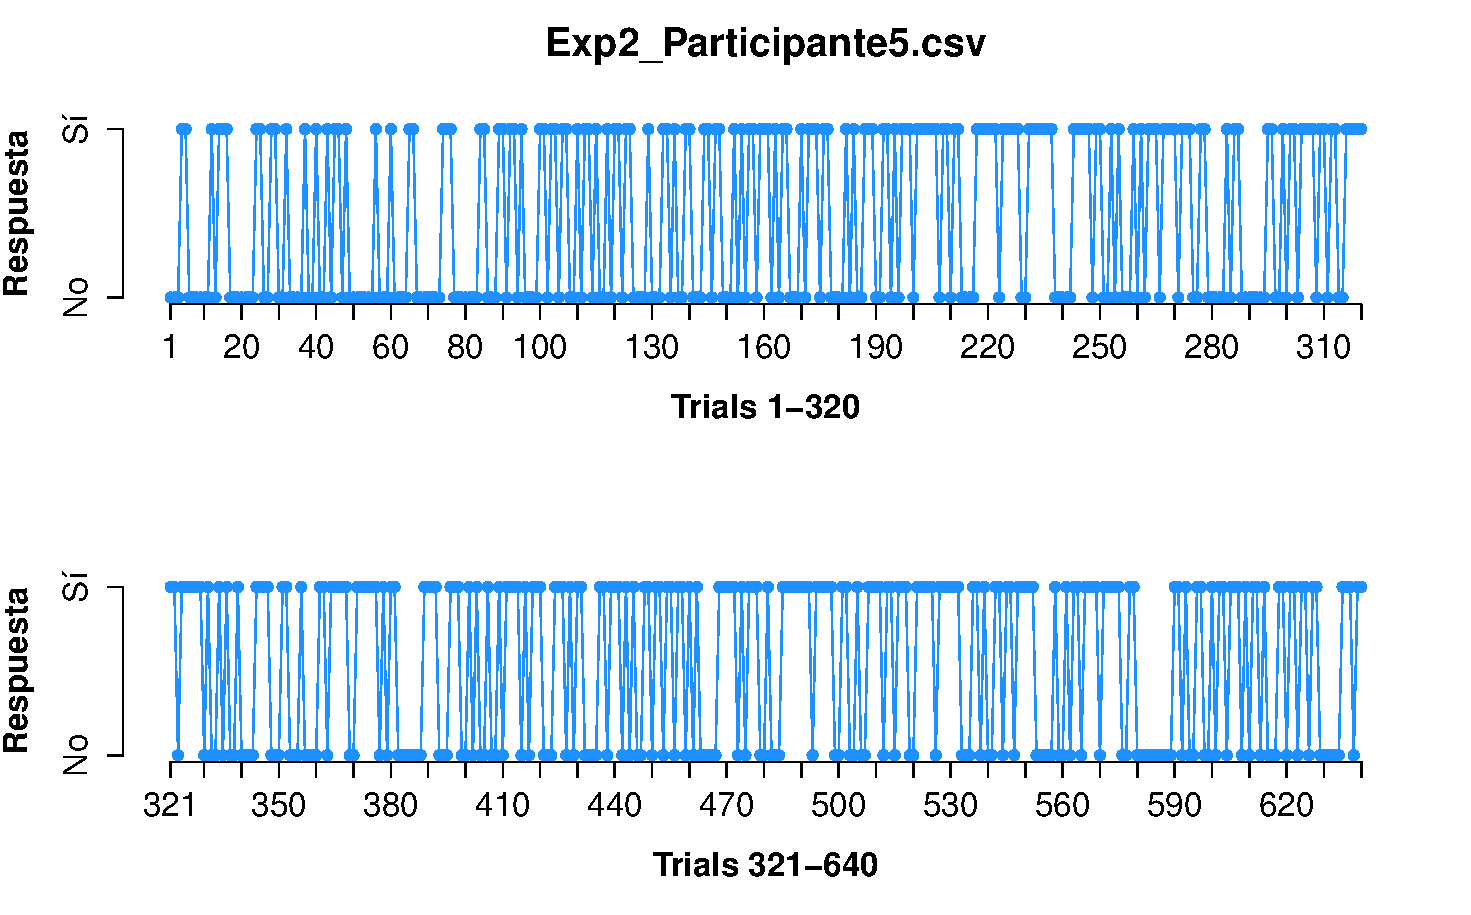
\includegraphics[width=0.30\textwidth]{Figures/Response_Exp2_P5} 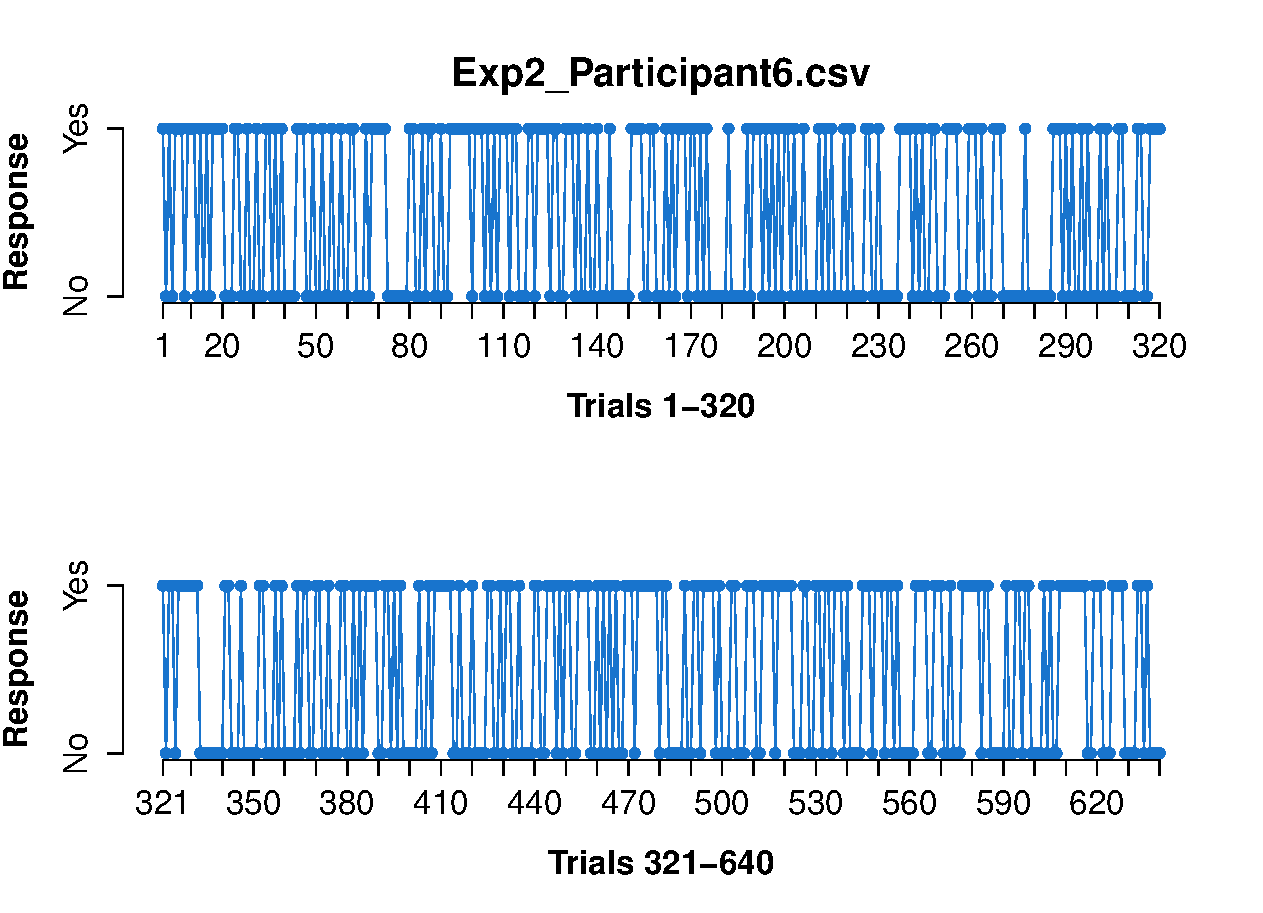
\includegraphics[width=0.30\textwidth]{Figures/Response_Exp2_P6}
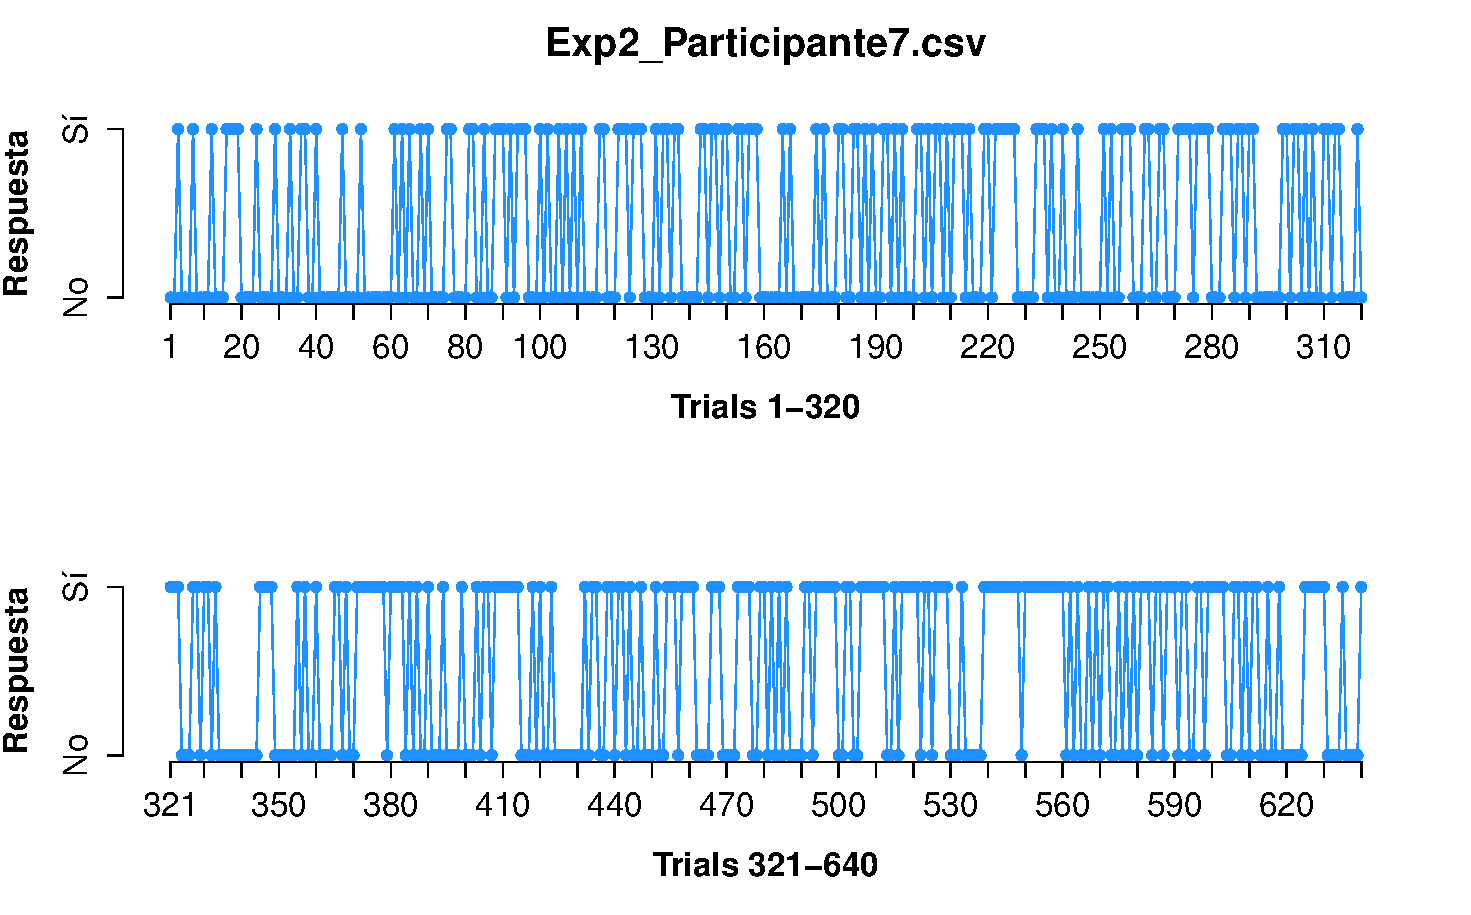
\includegraphics[width=0.30\textwidth]{Figures/Response_Exp2_P7} 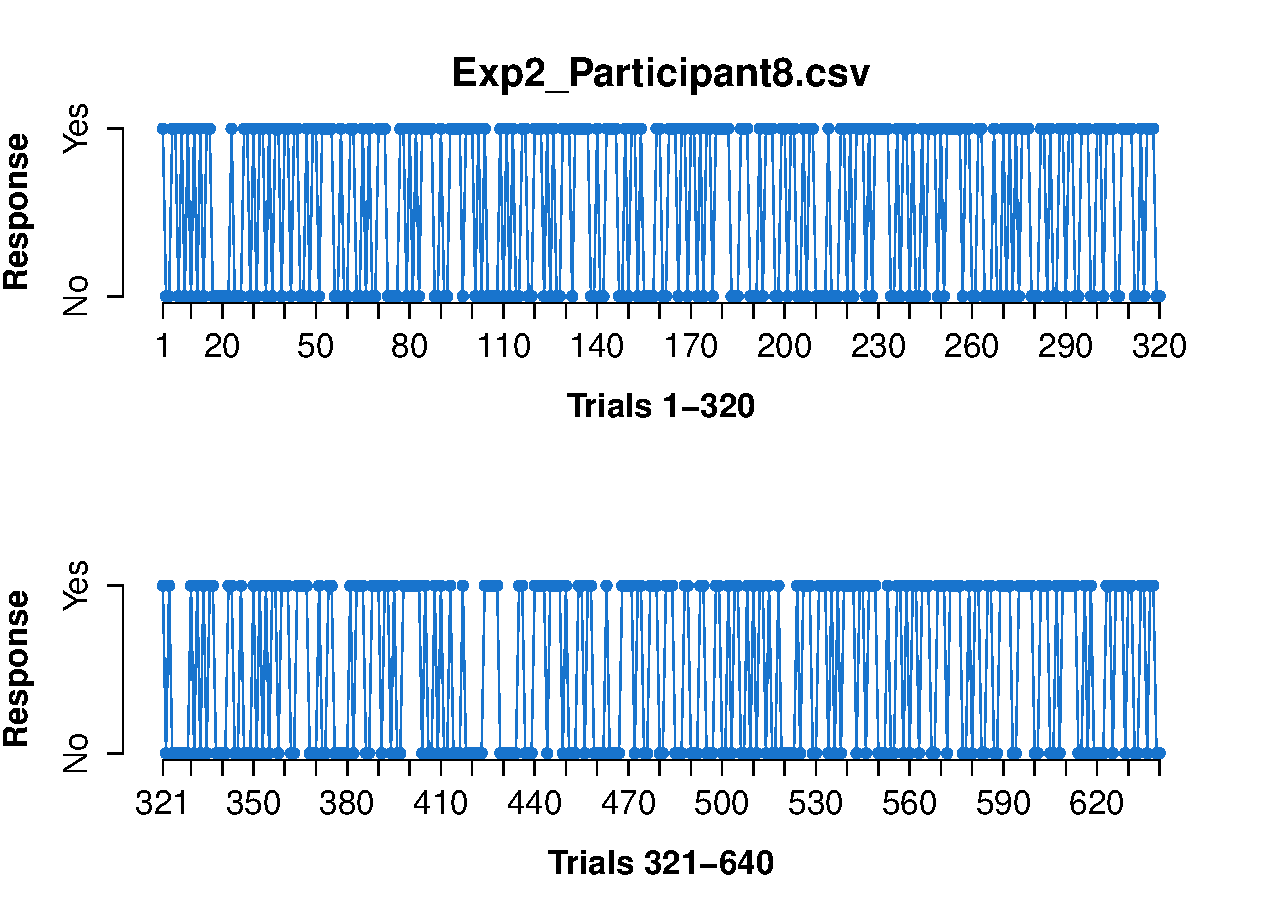
\includegraphics[width=0.30\textwidth]{Figures/Response_Exp2_P8} 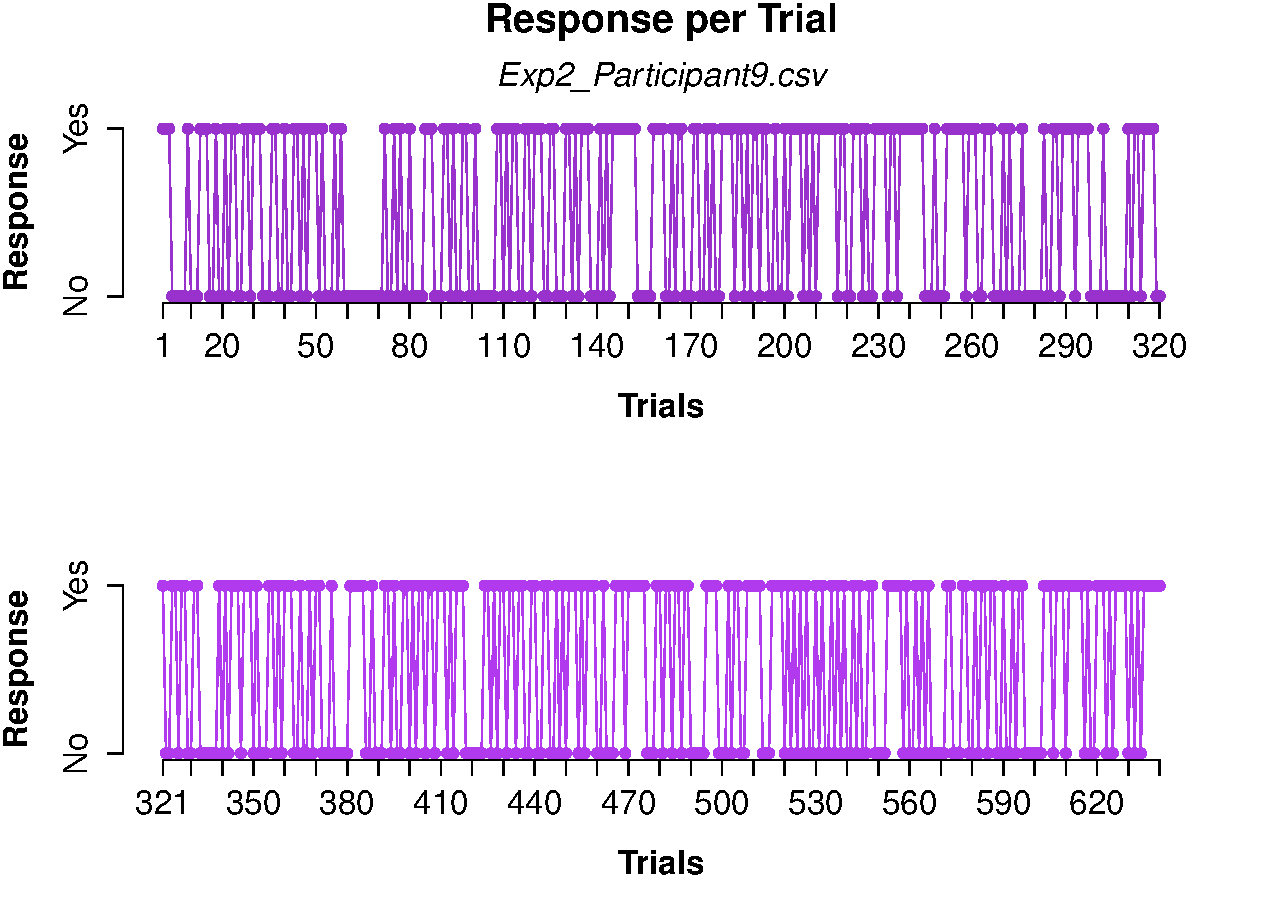
\includegraphics[width=0.30\textwidth]{Figures/Response_Exp2_P9}
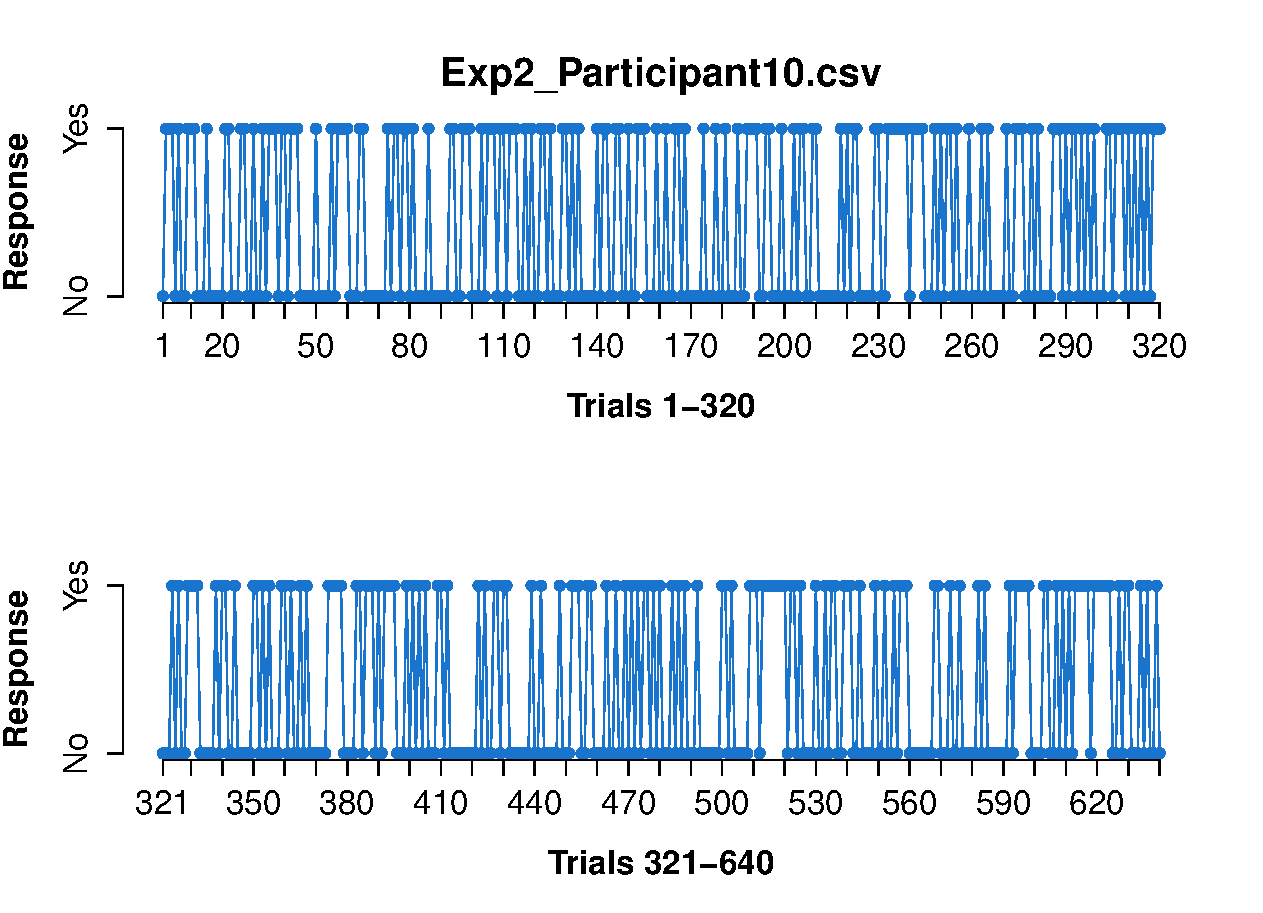
\includegraphics[width=0.30\textwidth]{Figures/Response_Exp2_P10} 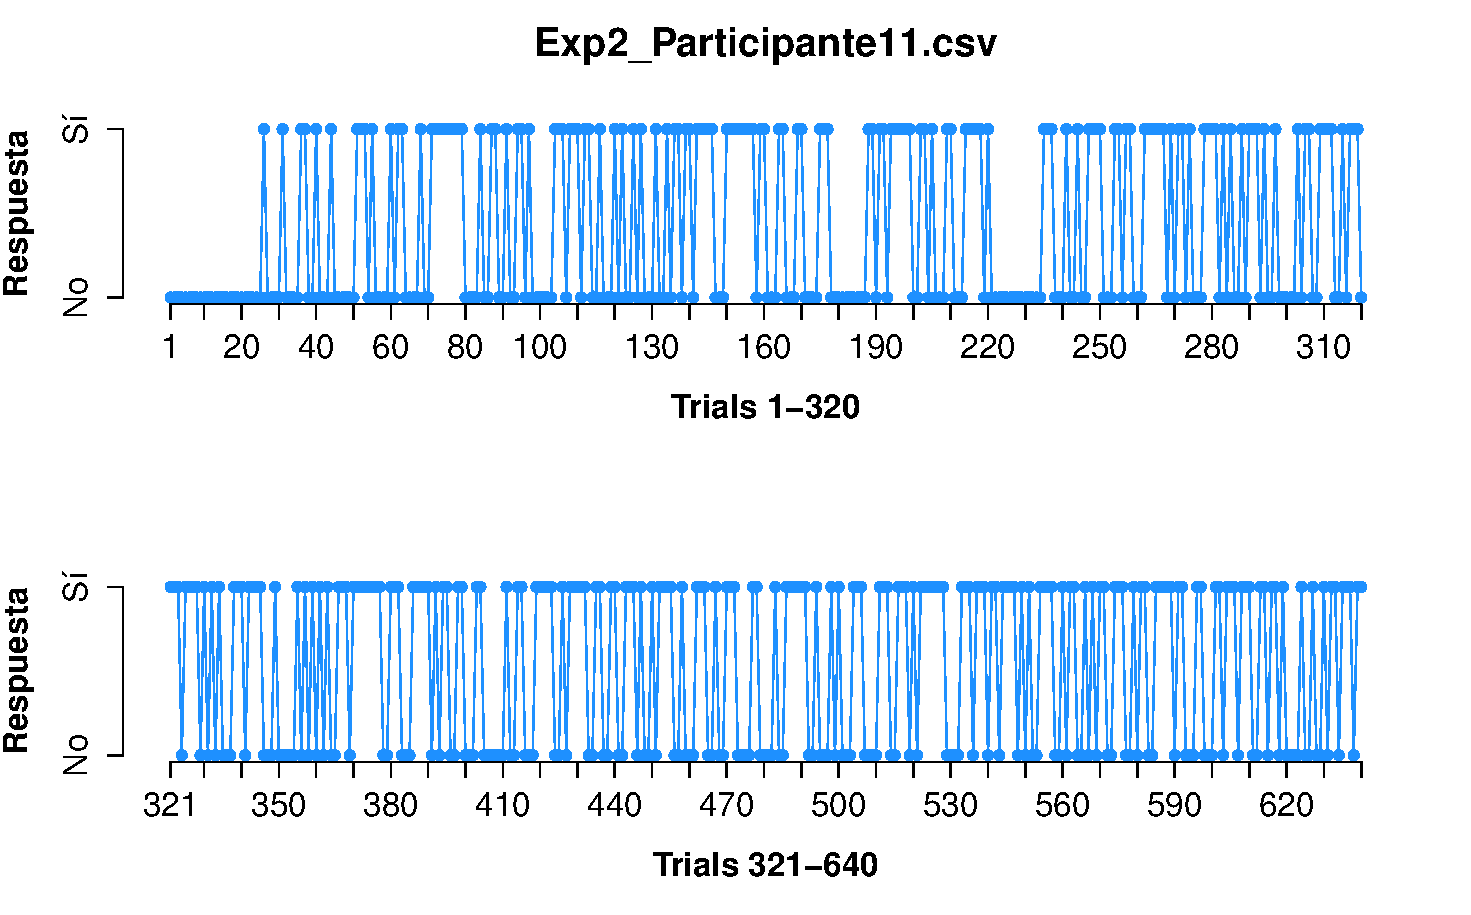
\includegraphics[width=0.30\textwidth]{Figures/Response_Exp2_P11} 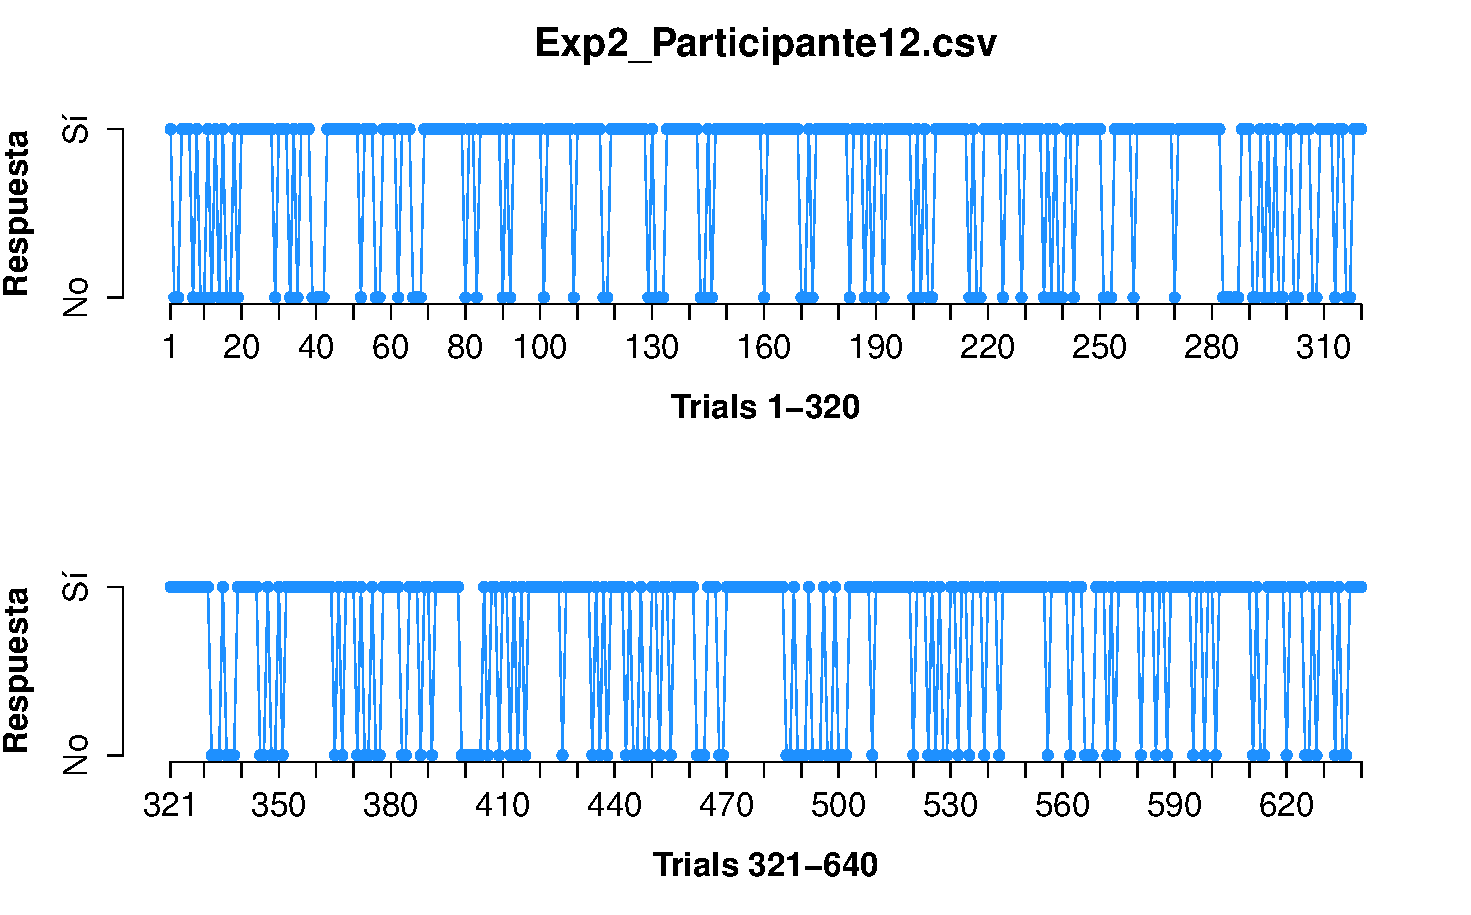
\includegraphics[width=0.30\textwidth]{Figures/Response_Exp2_P12}
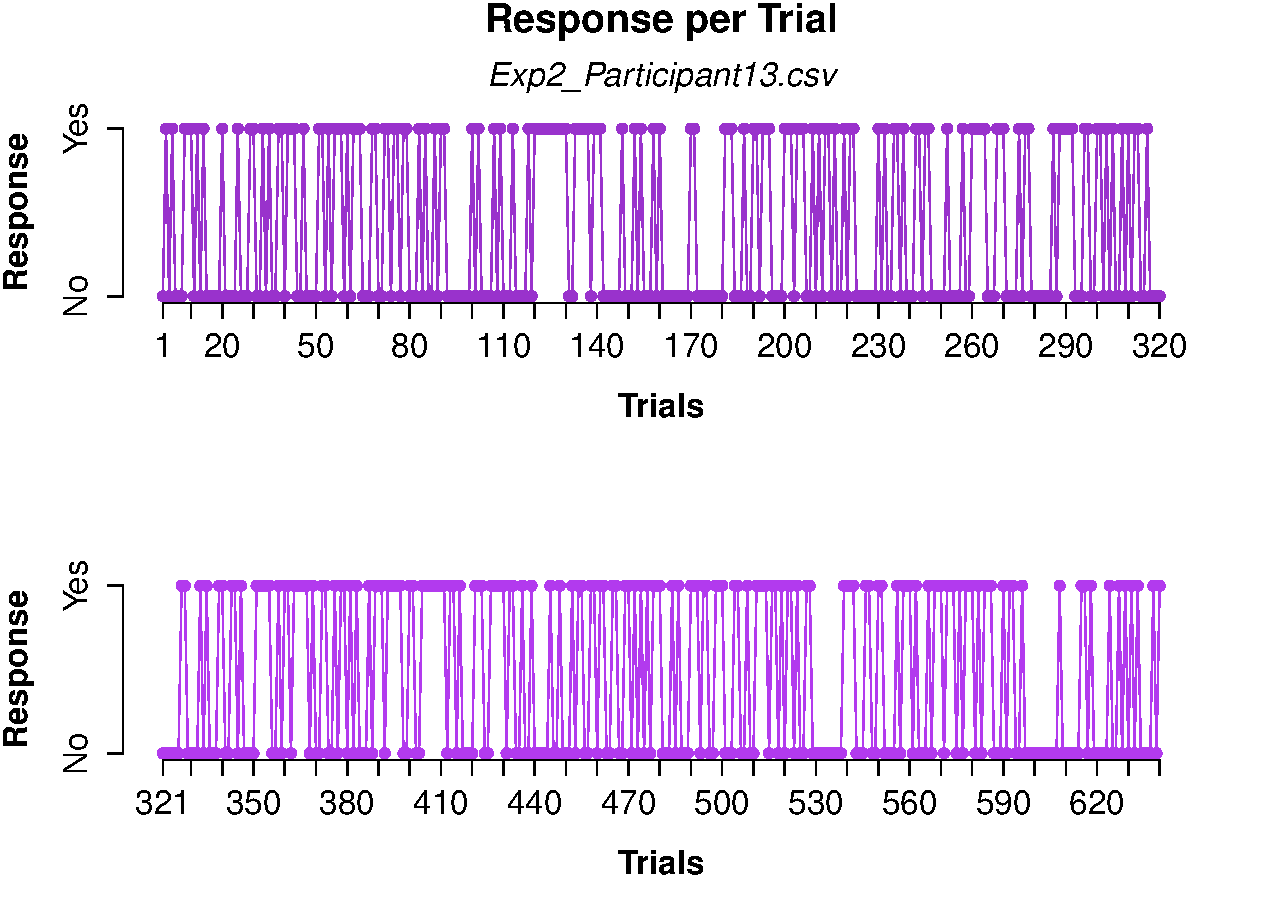
\includegraphics[width=0.30\textwidth]{Figures/Response_Exp2_P13} 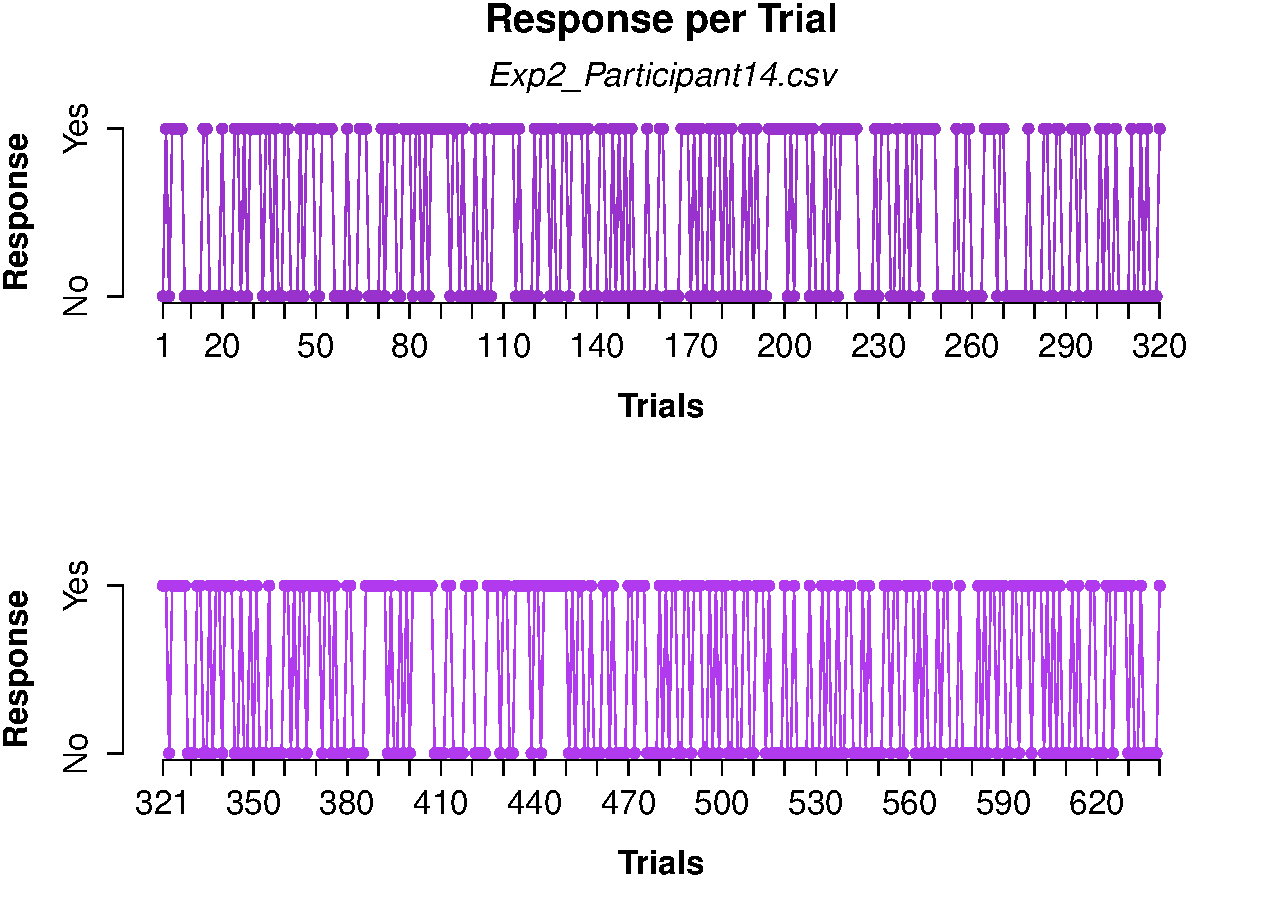
\includegraphics[width=0.30\textwidth]{Figures/Response_Exp2_P14} 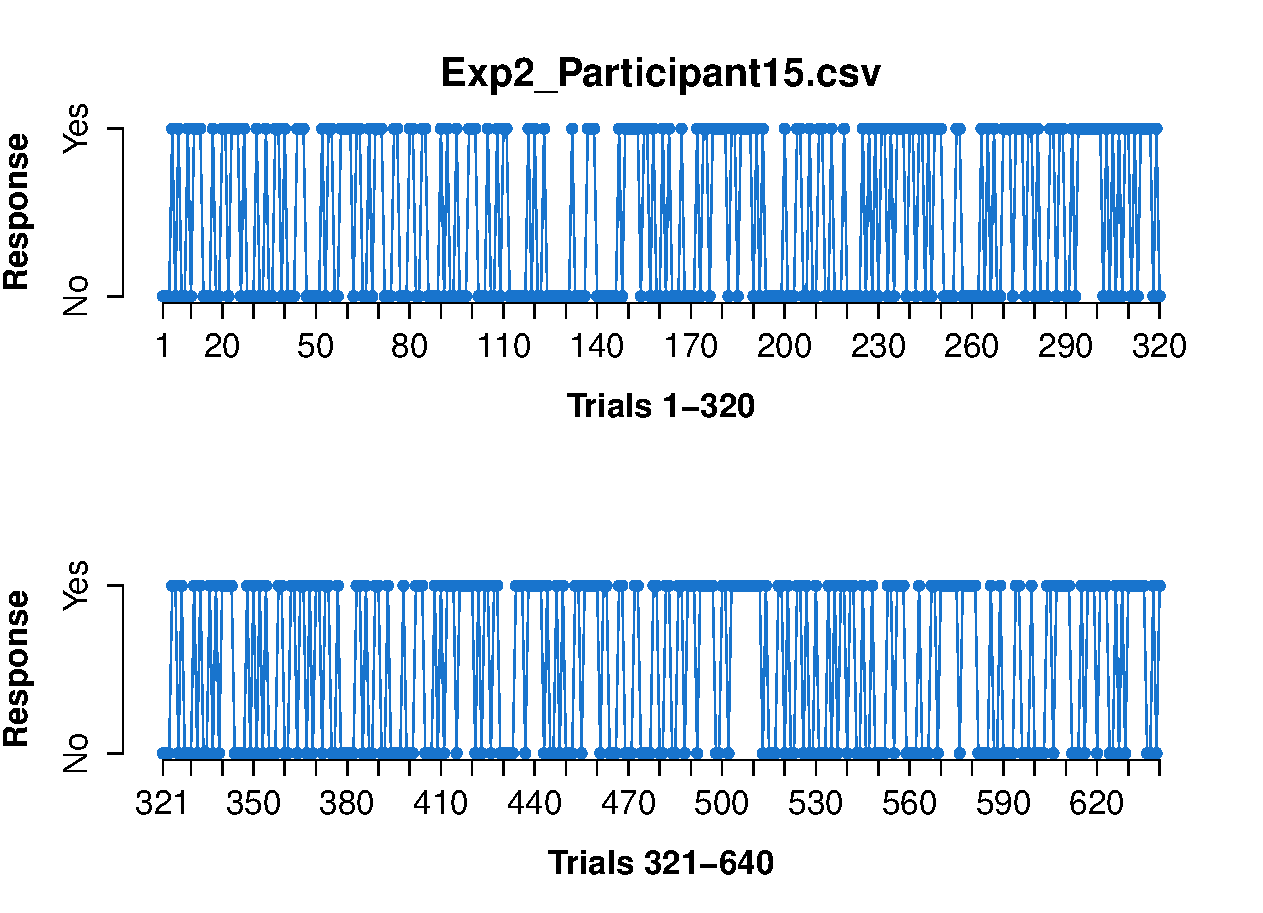
\includegraphics[width=0.30\textwidth]{Figures/Response_Exp2_P15}
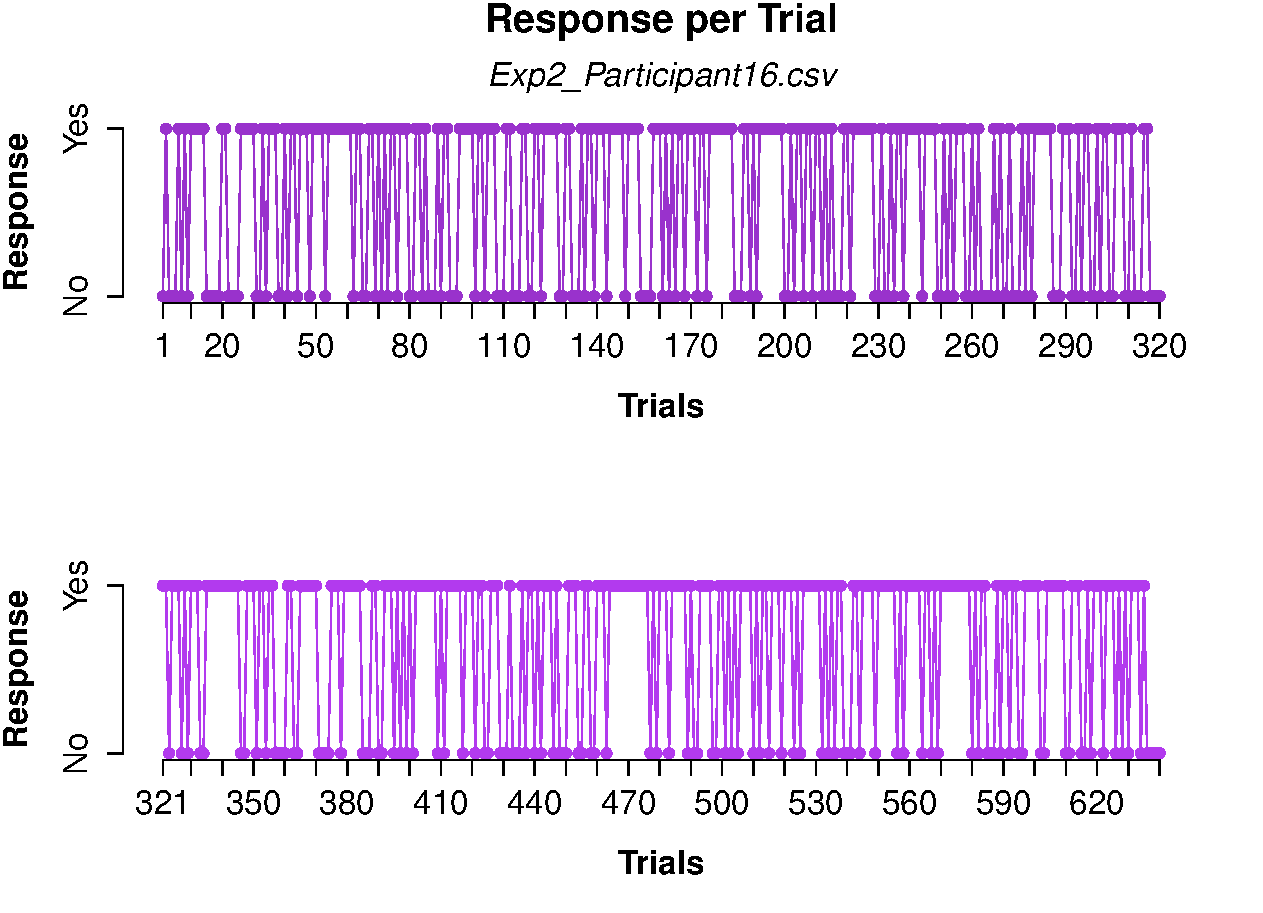
\includegraphics[width=0.30\textwidth]{Figures/Response_Exp2_P16} 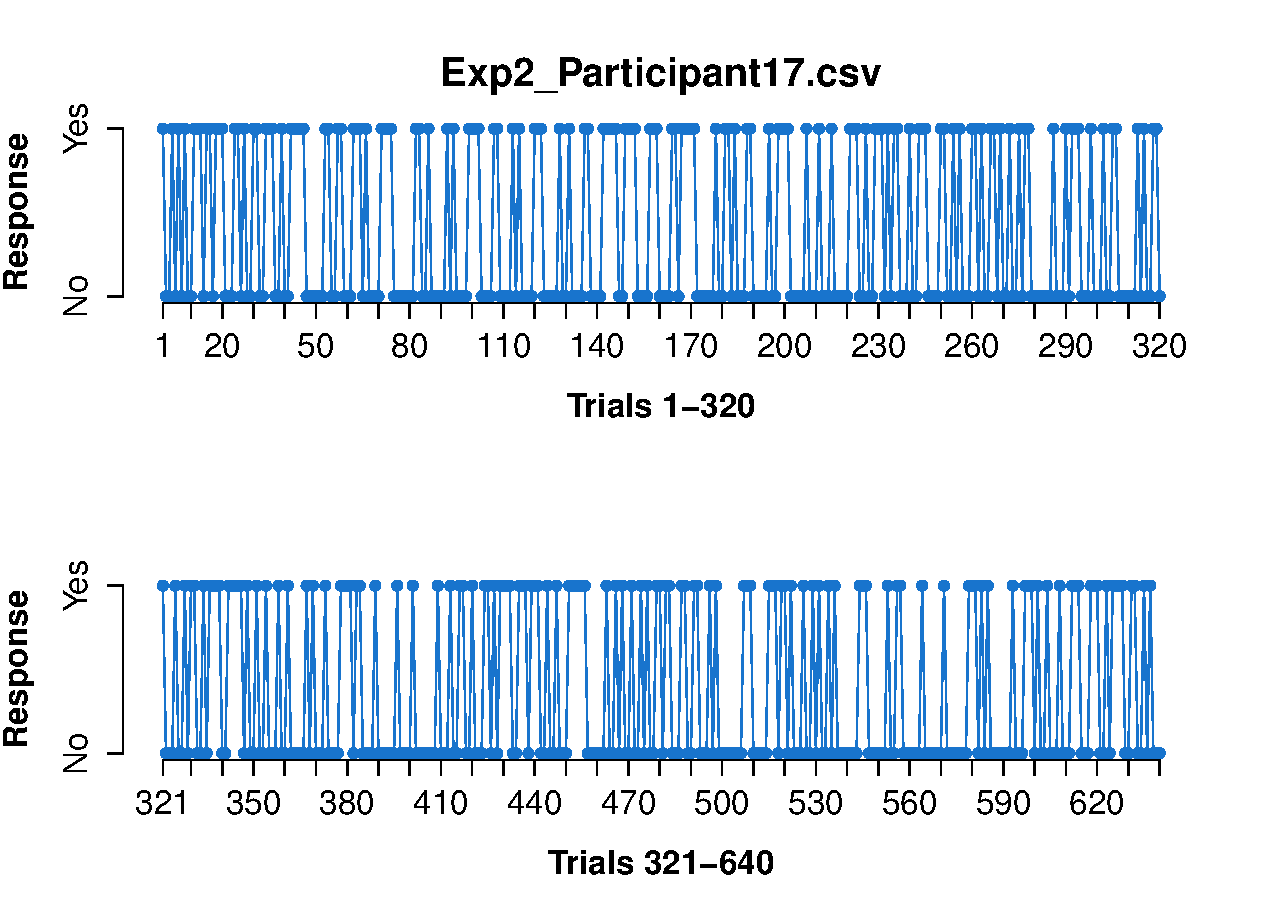
\includegraphics[width=0.30\textwidth]{Figures/Response_Exp2_P17} 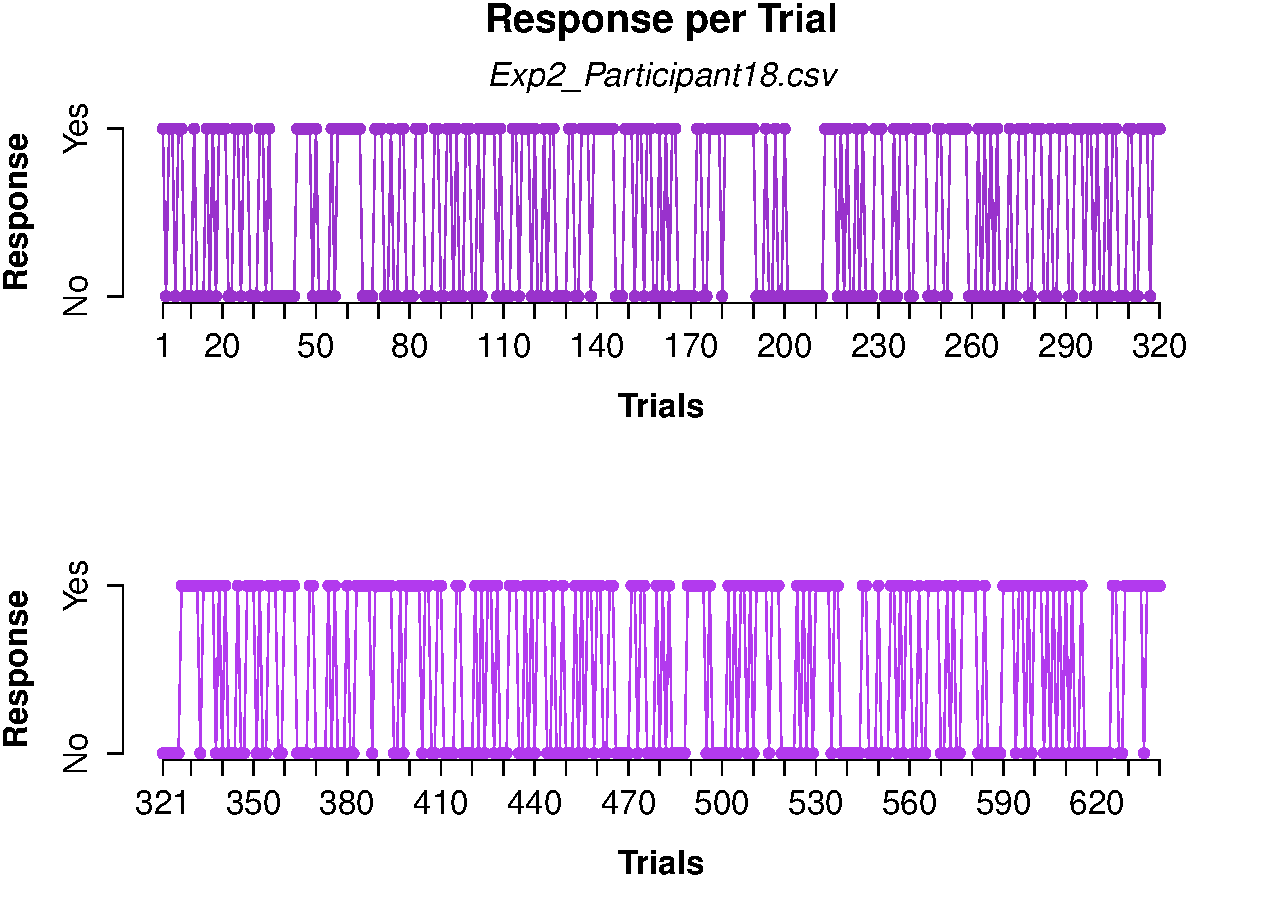
\includegraphics[width=0.30\textwidth]{Figures/Response_Exp2_P18}
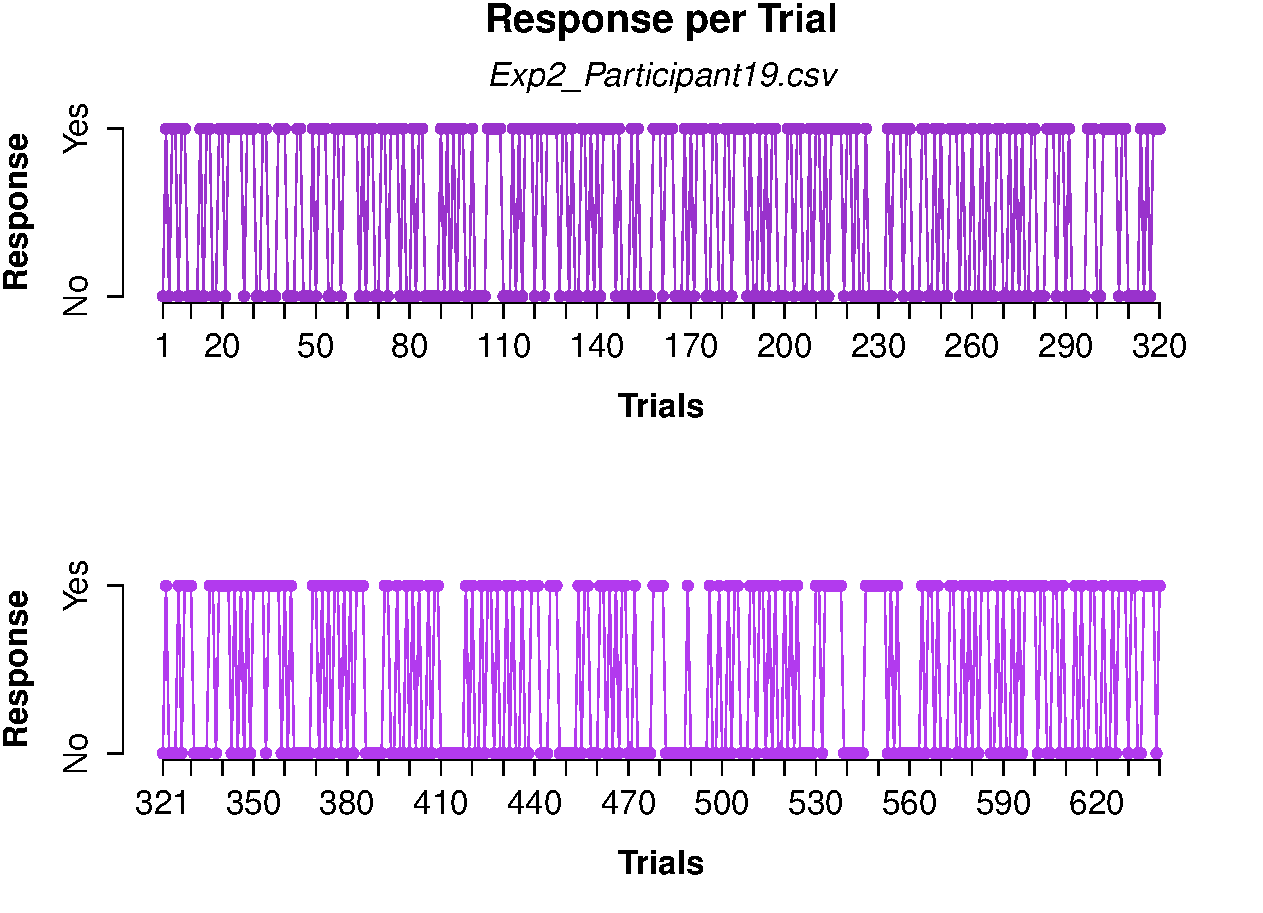
\includegraphics[width=0.30\textwidth]{Figures/Response_Exp2_P19} 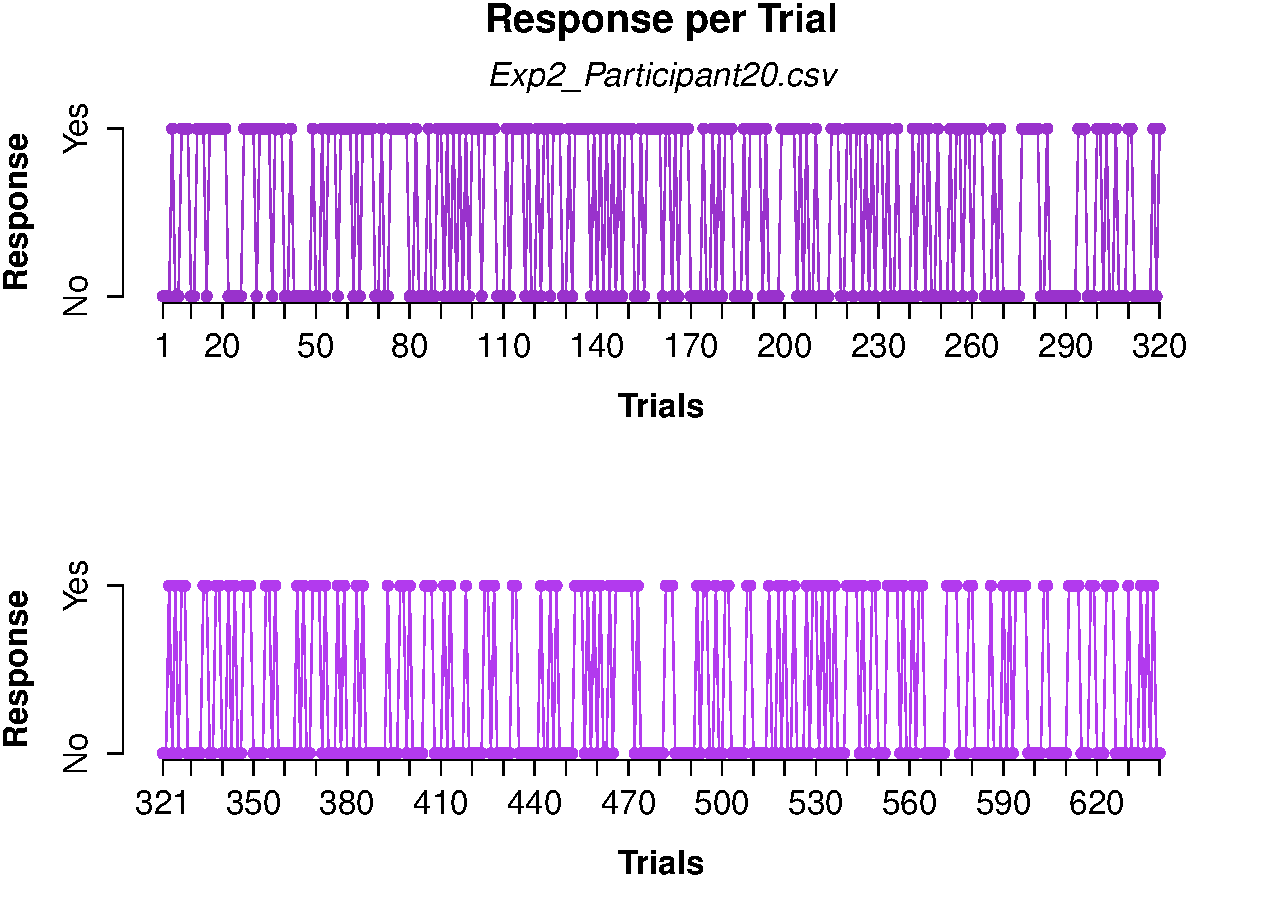
\includegraphics[width=0.30\textwidth]{Figures/Response_Exp2_P20} 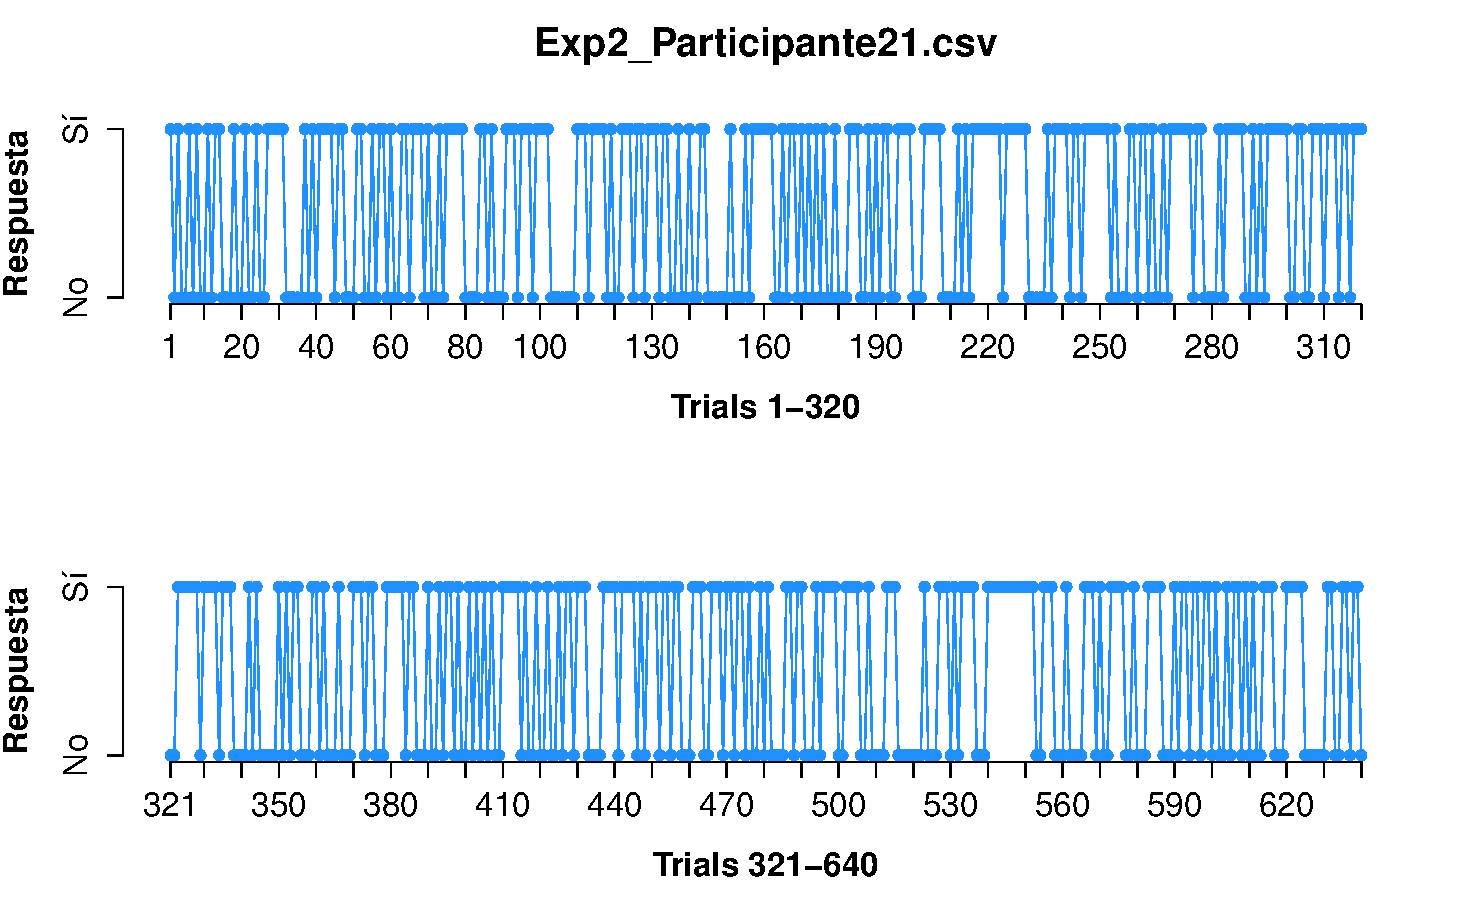
\includegraphics[width=0.30\textwidth]{Figures/Response_Exp2_P21} 
%\decoRule
\caption[Respuesta binaria registrada ensayo a ensayo; Experimento 2]{Respuestas registradas por ensayo en la tarea de detección binaria por cada uno de los veintiun participantes del Experimento 2. Las elecciones por participante se muestran en dos páneles que corresponden a los primeros y los últimos 320 ensayos del experimento (panel superior e inferior, respectivamente).}
\label{fig:Response_E2}
\end{figure}

\begin{figure}[th]
\centering
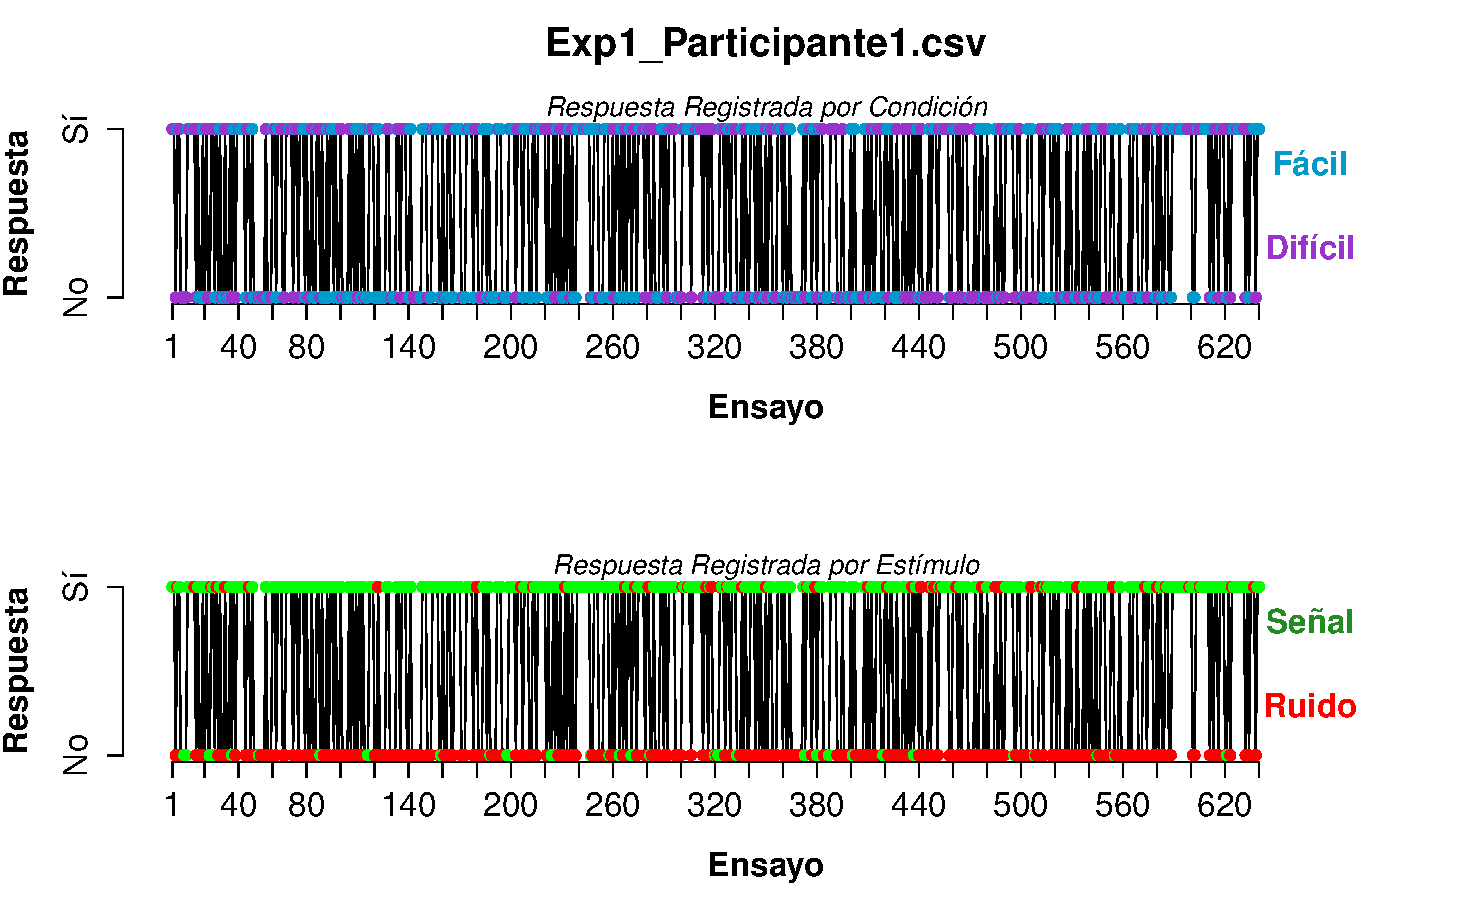
\includegraphics[width=0.30\textwidth]{Figures/BiasResp_Exp1_P1} 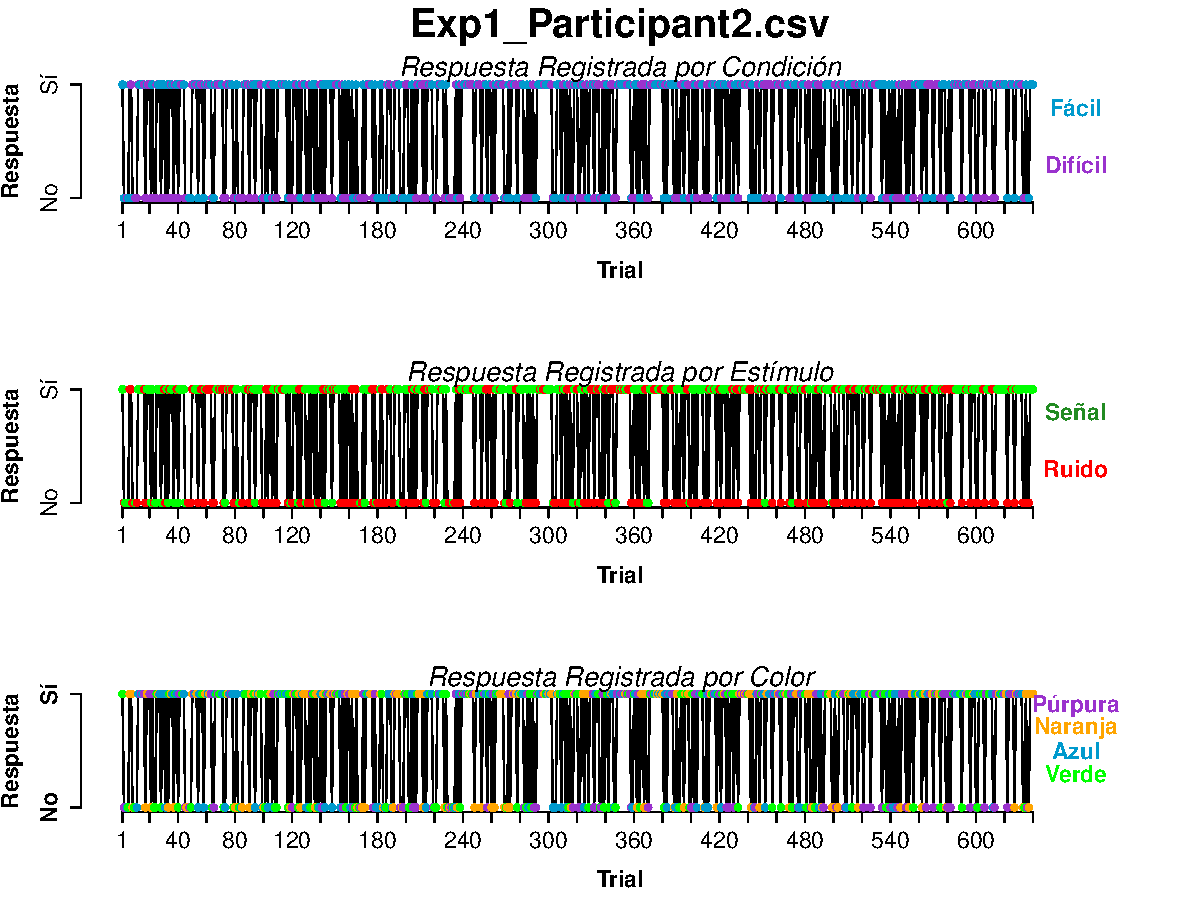
\includegraphics[width=0.30\textwidth]{Figures/BiasResp_Exp1_P2} 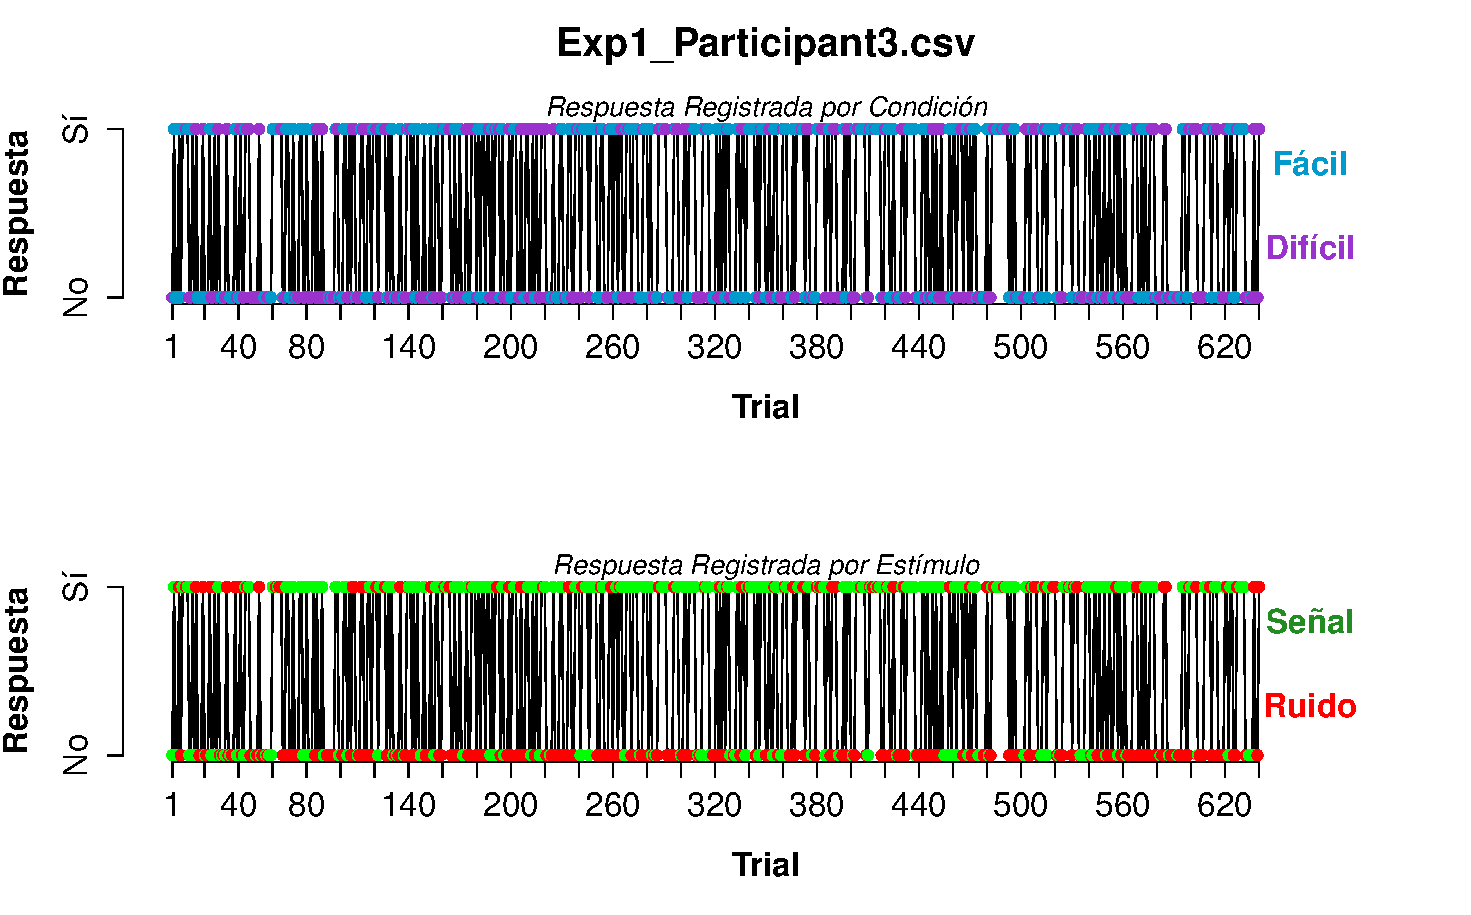
\includegraphics[width=0.30\textwidth]{Figures/BiasResp_Exp1_P3}
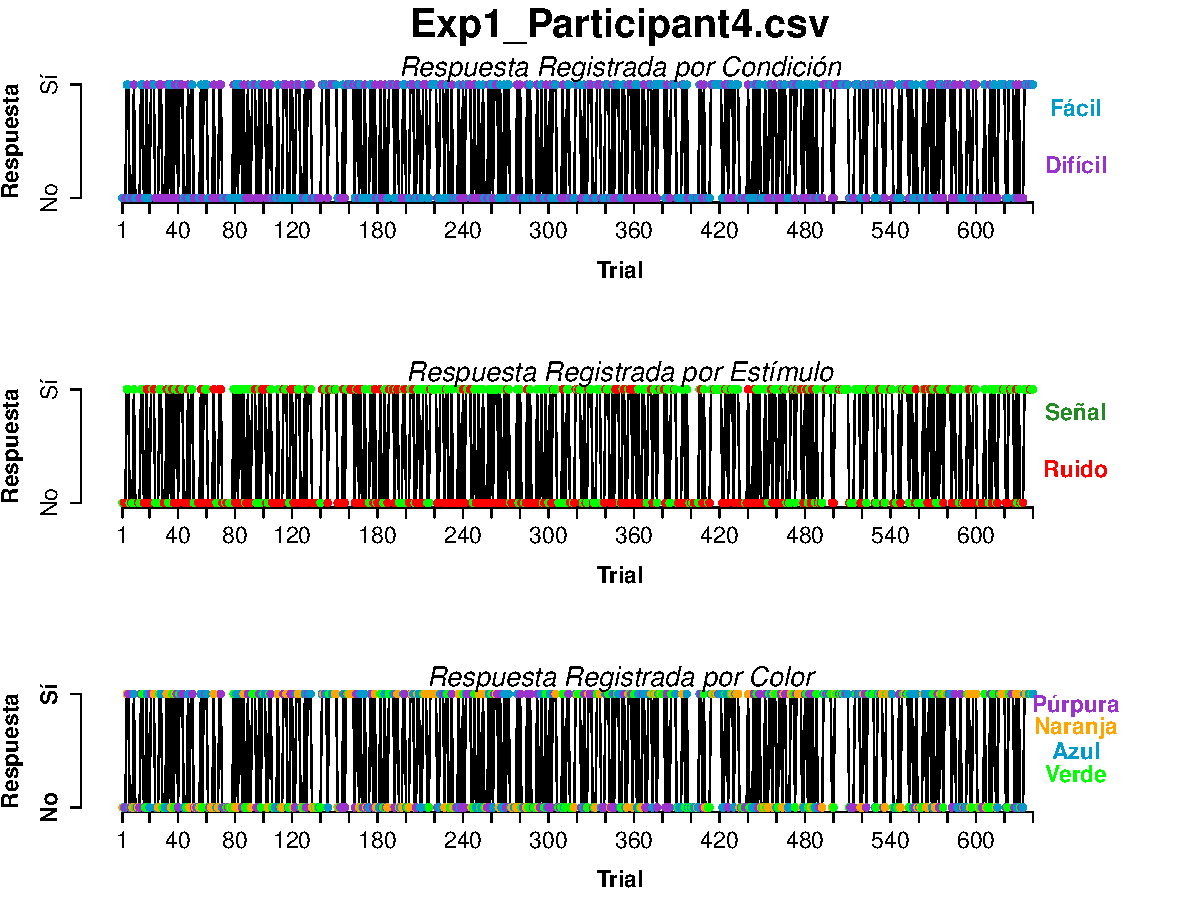
\includegraphics[width=0.30\textwidth]{Figures/BiasResp_Exp1_P4} 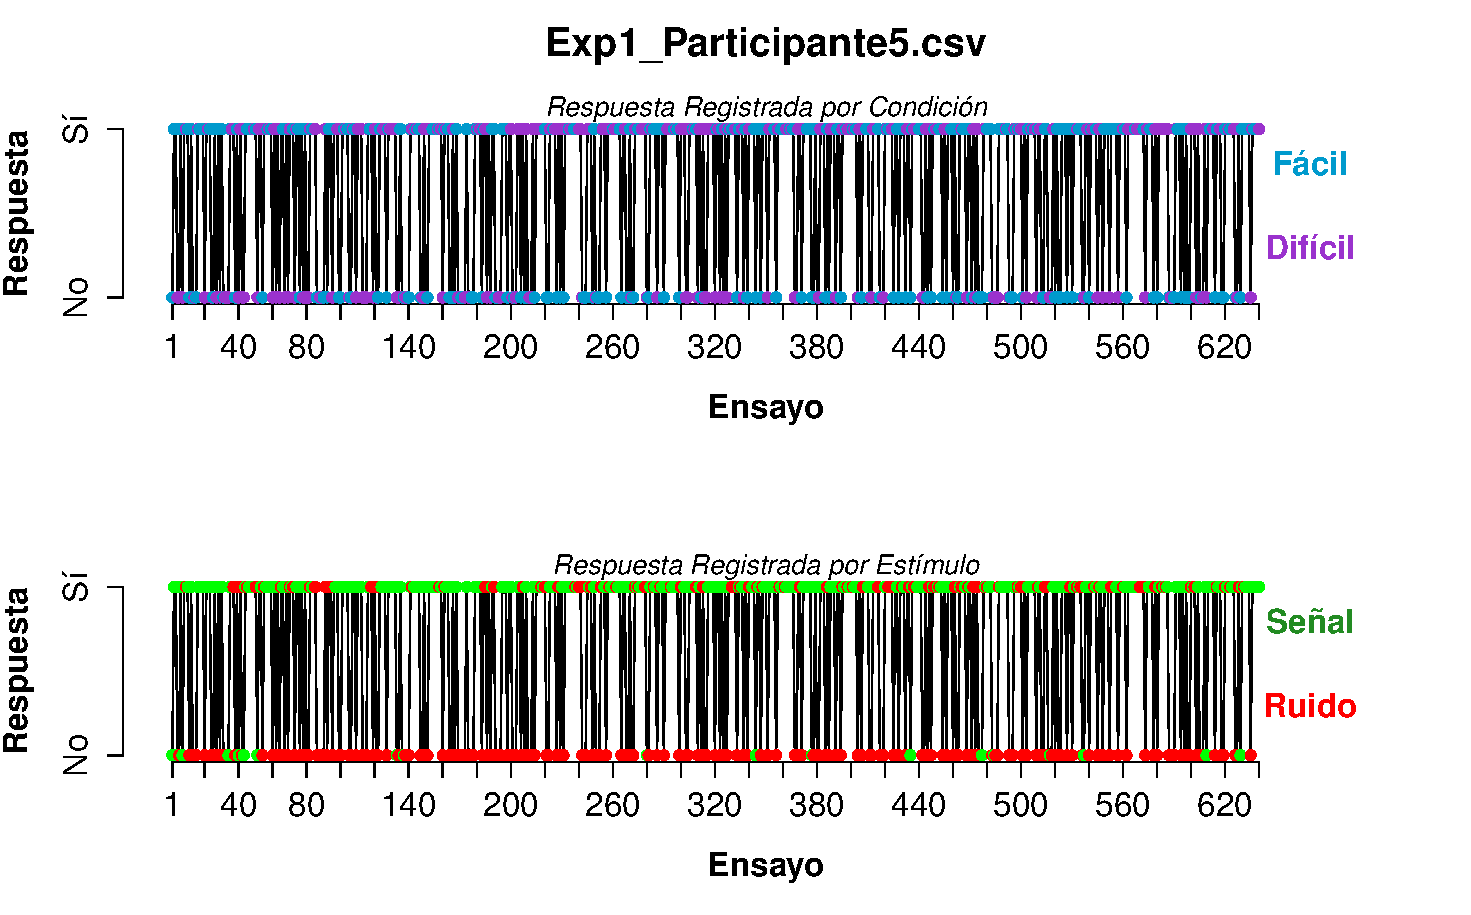
\includegraphics[width=0.30\textwidth]{Figures/BiasResp_Exp1_P5} 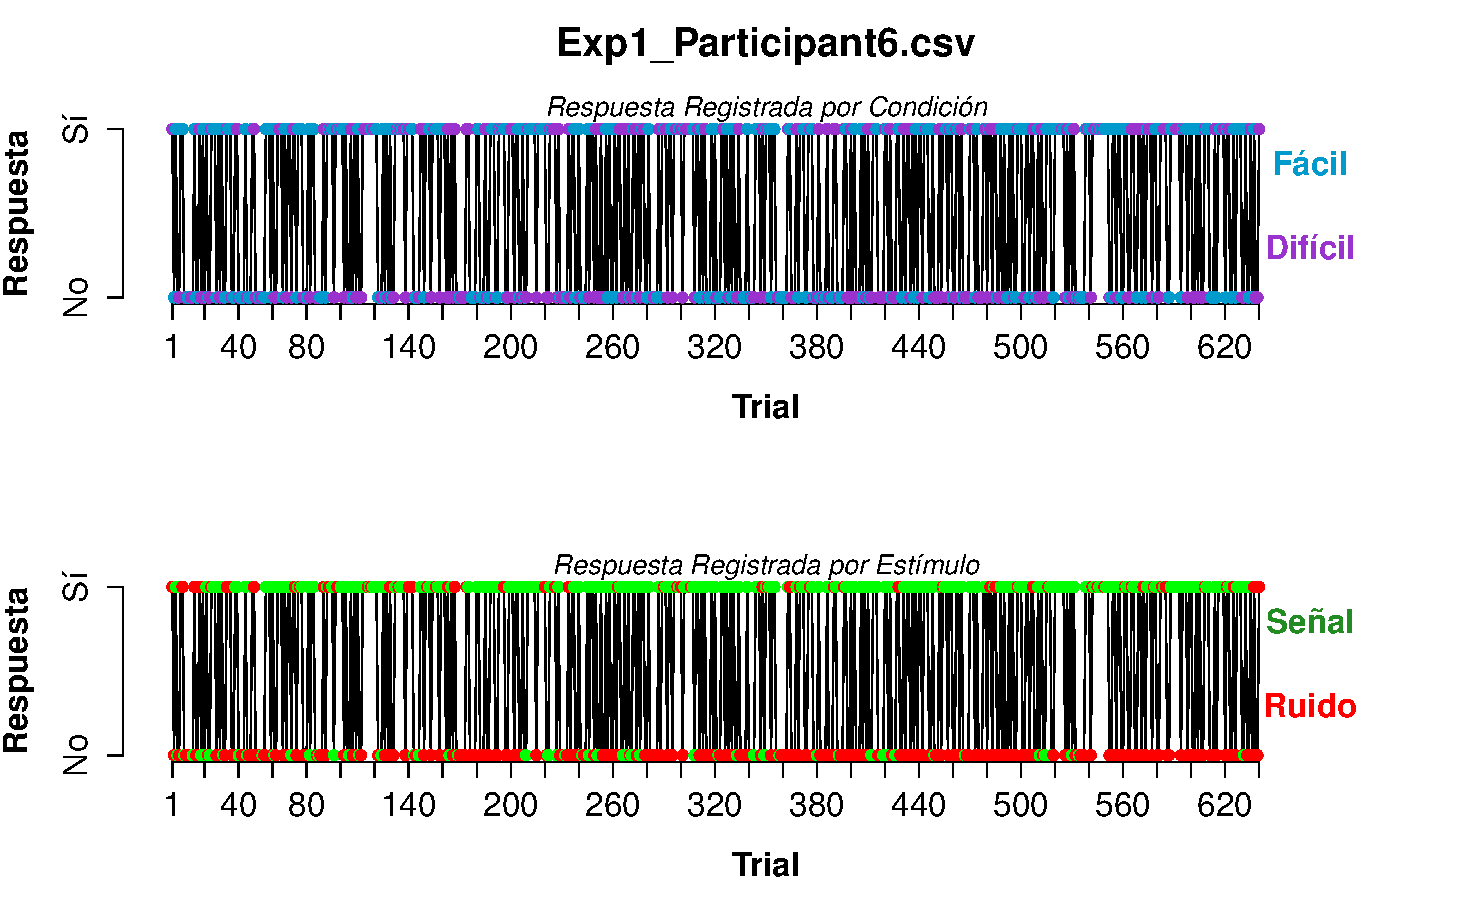
\includegraphics[width=0.30\textwidth]{Figures/BiasResp_Exp1_P6}
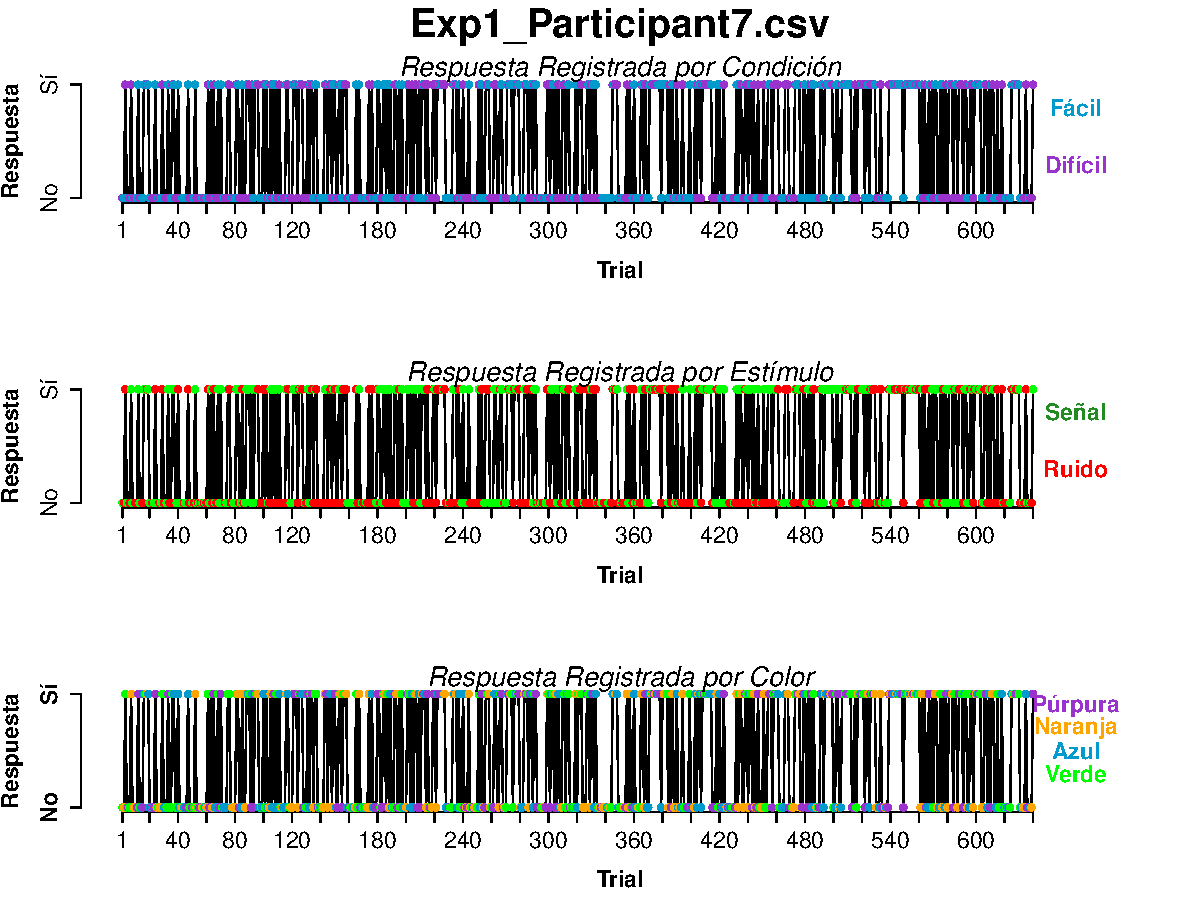
\includegraphics[width=0.30\textwidth]{Figures/BiasResp_Exp1_P7} 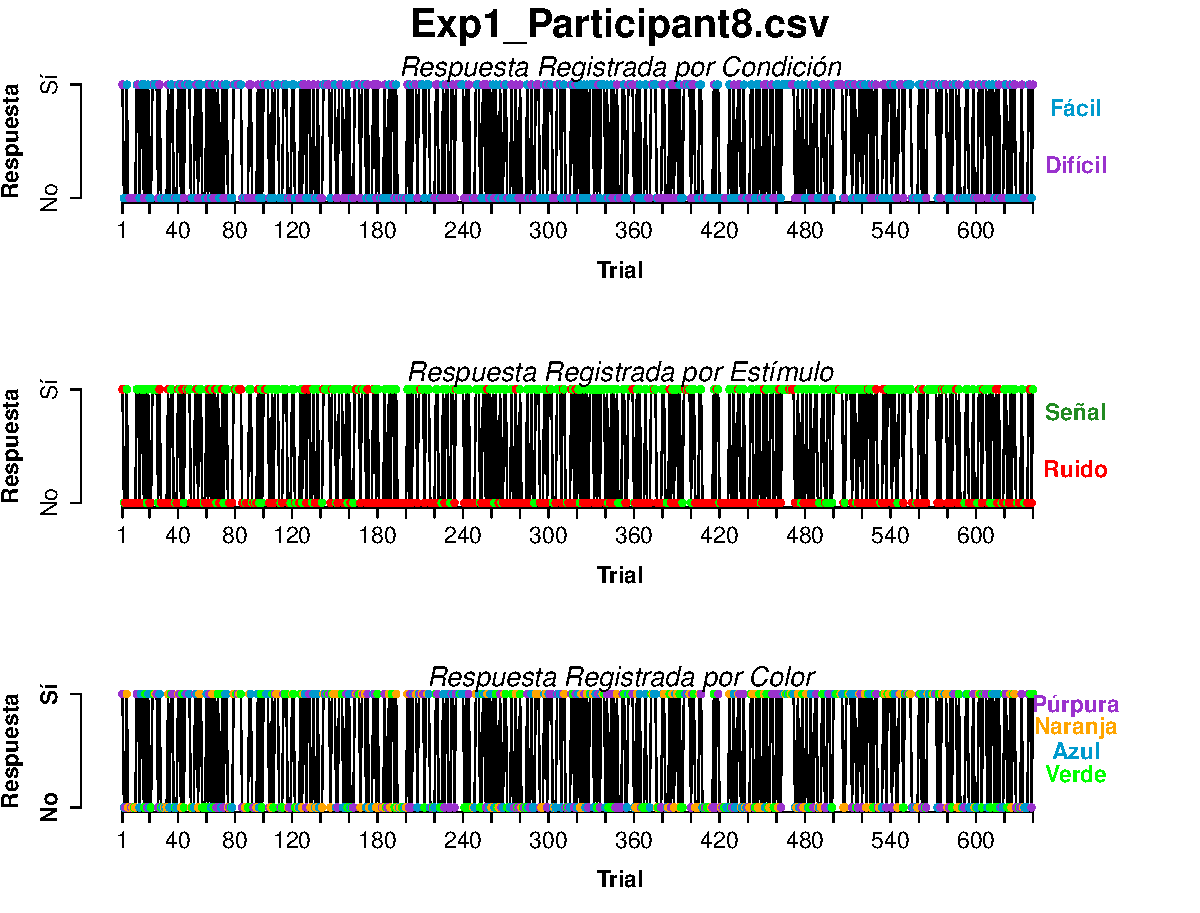
\includegraphics[width=0.30\textwidth]{Figures/BiasResp_Exp1_P8} 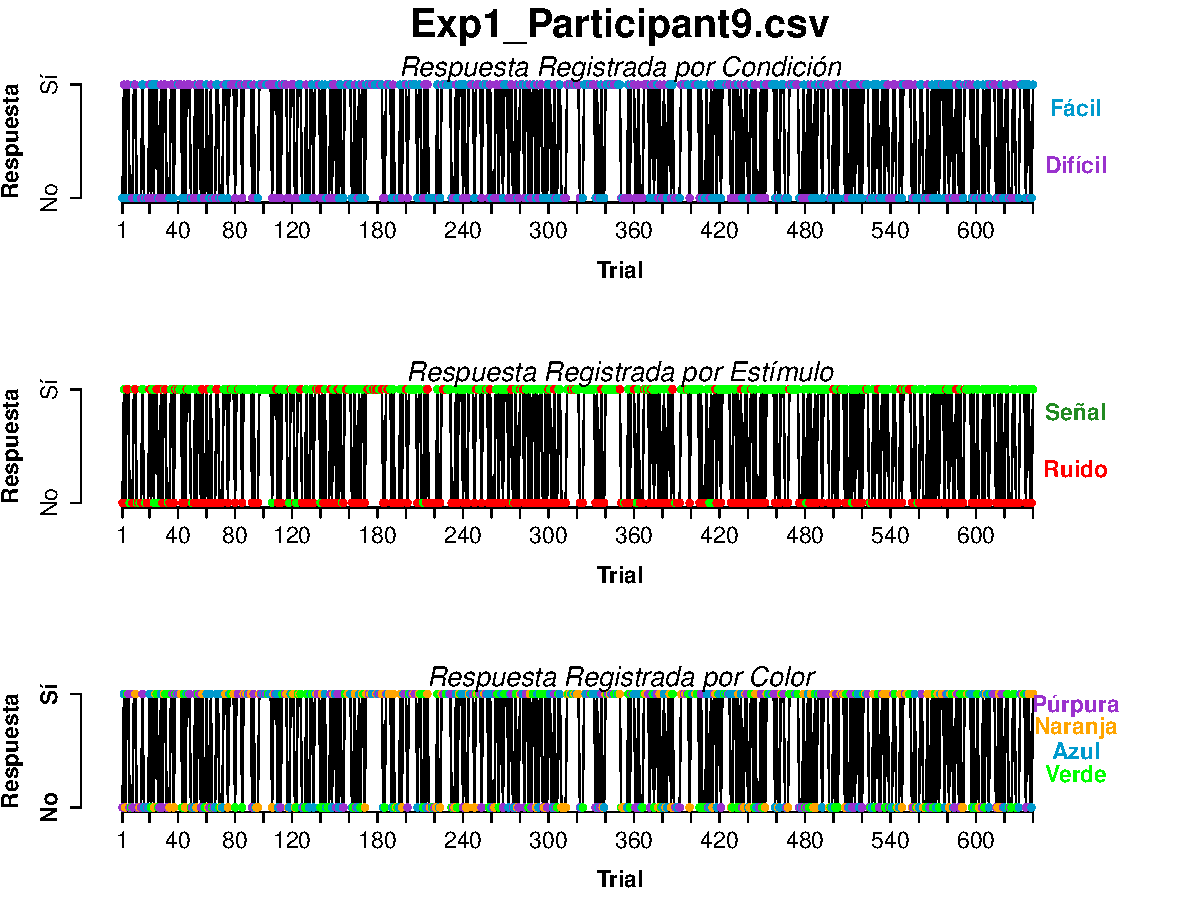
\includegraphics[width=0.30\textwidth]{Figures/BiasResp_Exp1_P9}
\includegraphics[width=0.30\textwidth]{Figures/BiasResp_Exp1_P10} \includegraphics[width=0.30\textwidth]{Figures/BiasResp_Exp1_P11} \includegraphics[width=0.30\textwidth]{Figures/BiasResp_Exp1_P12}
\includegraphics[width=0.30\textwidth]{Figures/BiasResp_Exp1_P13} \includegraphics[width=0.30\textwidth]{Figures/BiasResp_Exp1_P14} \includegraphics[width=0.30\textwidth]{Figures/BiasResp_Exp1_P15}
\includegraphics[width=0.30\textwidth]{Figures/BiasResp_Exp1_P16} \includegraphics[width=0.30\textwidth]{Figures/BiasResp_Exp1_P17} \includegraphics[width=0.30\textwidth]{Figures/BiasResp_Exp1_P18}
\includegraphics[width=0.30\textwidth]{Figures/BiasResp_Exp1_P19} \includegraphics[width=0.30\textwidth]{Figures/BiasResp_Exp1_P20} 
%\decoRule
\caption[Respuesta binaria registrada ensayo a ensayo en relación con el tipo de estímulo a evaluar; Experimento 1]{Respuesta registrada en cada ensayo para la tarea de detección binaria, por los veinte participantes del Experimento 1. Por cada participante se muestran dos gráficas que señalan con colores diferentes el tipo de estímulo presente en cada ensayo: En la parte superior, se señala si los estímulos eran de la condición fácil o difícil (con colores azul y violeta, respectivamente) y en la parte inferior, se distinguen los ensayos con señal y ruido presentándolos en color verde y rojo, respectivamente.}
\label{fig:BiasResp_E1}
\end{figure}

\begin{figure}[th]
\centering
\includegraphics[width=0.30\textwidth]{Figures/BiasResp_Exp2_P1} \includegraphics[width=0.30\textwidth]{Figures/BiasResp_Exp2_P2} \includegraphics[width=0.30\textwidth]{Figures/BiasResp_Exp2_P3}
\includegraphics[width=0.30\textwidth]{Figures/BiasResp_Exp2_P4} \includegraphics[width=0.30\textwidth]{Figures/BiasResp_Exp2_P5} \includegraphics[width=0.30\textwidth]{Figures/BiasResp_Exp2_P6}
\includegraphics[width=0.30\textwidth]{Figures/BiasResp_Exp2_P7} \includegraphics[width=0.30\textwidth]{Figures/BiasResp_Exp2_P8} \includegraphics[width=0.30\textwidth]{Figures/BiasResp_Exp2_P9}
\includegraphics[width=0.30\textwidth]{Figures/BiasResp_Exp2_P10} \includegraphics[width=0.30\textwidth]{Figures/BiasResp_Exp2_P11} \includegraphics[width=0.30\textwidth]{Figures/BiasResp_Exp2_P12}
\includegraphics[width=0.30\textwidth]{Figures/BiasResp_Exp2_P13} \includegraphics[width=0.30\textwidth]{Figures/BiasResp_Exp2_P14} \includegraphics[width=0.30\textwidth]{Figures/BiasResp_Exp2_P15}
\includegraphics[width=0.30\textwidth]{Figures/BiasResp_Exp2_P16} \includegraphics[width=0.30\textwidth]{Figures/BiasResp_Exp2_P17} \includegraphics[width=0.30\textwidth]{Figures/BiasResp_Exp2_P18}
\includegraphics[width=0.30\textwidth]{Figures/BiasResp_Exp2_P19} \includegraphics[width=0.30\textwidth]{Figures/BiasResp_Exp2_P20} \includegraphics[width=0.30\textwidth]{Figures/BiasResp_Exp2_P21}
%\decoRule
\caption[Respuesta binaria registrada ensayo a ensayo en relación con el tipo de estímulo a evaluar; Experimento 2]{Respuesta registrada por ensayo en la tarea de detección binaria por los veintiun participantes del Experimento 2. Por cada participante se muestran dos gráficas que señalan con colores diferentes el tipo de estímulo evaluado en cada ensayo: En la parte superior, se señala la condición de dificultad (azul para fácil y violeta para difícil) y en la parte inferior, el tipo de ensayo (las señales en verde y en rojo los ensayos con ruido).}
\label{fig:BiasResp_E2}
\end{figure}

\begin{figure}[th]
\centering
\includegraphics[width=0.30\textwidth]{Figures/Rating_Exp1_P1} \includegraphics[width=0.30\textwidth]{Figures/Rating_Exp1_P2} \includegraphics[width=0.30\textwidth]{Figures/Rating_Exp1_P3}
\includegraphics[width=0.30\textwidth]{Figures/Rating_Exp1_P4} \includegraphics[width=0.30\textwidth]{Figures/Rating_Exp1_P5} \includegraphics[width=0.30\textwidth]{Figures/Rating_Exp1_P6}
\includegraphics[width=0.30\textwidth]{Figures/Rating_Exp1_P7} \includegraphics[width=0.30\textwidth]{Figures/Rating_Exp1_P8} \includegraphics[width=0.30\textwidth]{Figures/Rating_Exp1_P9}
\includegraphics[width=0.30\textwidth]{Figures/Rating_Exp1_P10} \includegraphics[width=0.30\textwidth]{Figures/Rating_Exp1_P11} \includegraphics[width=0.30\textwidth]{Figures/Rating_Exp1_P12}
\includegraphics[width=0.30\textwidth]{Figures/Rating_Exp1_P13} \includegraphics[width=0.30\textwidth]{Figures/Rating_Exp1_P14} \includegraphics[width=0.30\textwidth]{Figures/Rating_Exp1_P15}
\includegraphics[width=0.30\textwidth]{Figures/Rating_Exp1_P16} \includegraphics[width=0.30\textwidth]{Figures/Rating_Exp1_P17} \includegraphics[width=0.30\textwidth]{Figures/Rating_Exp1_P18}
\includegraphics[width=0.30\textwidth]{Figures/Rating_Exp1_P19} \includegraphics[width=0.30\textwidth]{Figures/Rating_Exp1_P20} 
%\decoRule
\caption[Puntajes de Confianza asignados ensayo a ensayo; Experimento 1]{Puntaje de confianza asignado a las respuestas binarias emitidas ensayo a ensayo por cada participante del Experimento 1. Se despliegan las elecciones de cada participante un panel superior e inferior, que presentan los primeros y los últimos 320 ensayos del experimento, respectivamente.}
\label{fig:Rating_E1}
\end{figure}

\begin{figure}[th]
\centering
\includegraphics[width=0.30\textwidth]{Figures/Rating_Exp2_P1} \includegraphics[width=0.30\textwidth]{Figures/Rating_Exp2_P2} \includegraphics[width=0.30\textwidth]{Figures/Rating_Exp2_P3}
\includegraphics[width=0.30\textwidth]{Figures/Rating_Exp2_P4} \includegraphics[width=0.30\textwidth]{Figures/Rating_Exp2_P5} \includegraphics[width=0.30\textwidth]{Figures/Rating_Exp2_P6}
\includegraphics[width=0.30\textwidth]{Figures/Rating_Exp2_P7} \includegraphics[width=0.30\textwidth]{Figures/Rating_Exp2_P8} \includegraphics[width=0.30\textwidth]{Figures/Rating_Exp2_P9}
\includegraphics[width=0.30\textwidth]{Figures/Rating_Exp2_P10} \includegraphics[width=0.30\textwidth]{Figures/Rating_Exp2_P11} \includegraphics[width=0.30\textwidth]{Figures/Rating_Exp2_P12}
\includegraphics[width=0.30\textwidth]{Figures/Rating_Exp2_P13} \includegraphics[width=0.30\textwidth]{Figures/Rating_Exp2_P14} \includegraphics[width=0.30\textwidth]{Figures/Rating_Exp2_P15}
\includegraphics[width=0.30\textwidth]{Figures/Rating_Exp2_P16} \includegraphics[width=0.30\textwidth]{Figures/Rating_Exp2_P17} \includegraphics[width=0.30\textwidth]{Figures/Rating_Exp2_P18}
\includegraphics[width=0.30\textwidth]{Figures/Rating_Exp2_P19} \includegraphics[width=0.30\textwidth]{Figures/Rating_Exp2_P20} \includegraphics[width=0.30\textwidth]{Figures/Rating_Exp2_P21}
%\decoRule
\caption[Puntajes de Confianza asignados ensayo a ensayo; Experimento 2]{Puntaje de confianza asignado a las respuestas binarias emitidas ensayo a ensayo por cada participante del Experimento 1. Se despliegan las elecciones de cada participante un panel superior e inferior, que presentan los primeros y los últimos 320 ensayos del experimento, respectivamente.}
\label{fig:Rating_E2}
\end{figure}











\begin{figure}[th]
\centering
\includegraphics[width=0.30\textwidth]{Figures/Success_Exp1_P1} \includegraphics[width=0.30\textwidth]{Figures/Success_Exp1_P2} \includegraphics[width=0.30\textwidth]{Figures/Success_Exp1_P3}
\includegraphics[width=0.30\textwidth]{Figures/Success_Exp1_P4} \includegraphics[width=0.30\textwidth]{Figures/Success_Exp1_P5} \includegraphics[width=0.30\textwidth]{Figures/Success_Exp1_P6}
\includegraphics[width=0.30\textwidth]{Figures/Success_Exp1_P7} \includegraphics[width=0.30\textwidth]{Figures/Success_Exp1_P8} \includegraphics[width=0.30\textwidth]{Figures/Success_Exp1_P9}
\includegraphics[width=0.30\textwidth]{Figures/Success_Exp1_P10} \includegraphics[width=0.30\textwidth]{Figures/Success_Exp1_P11} \includegraphics[width=0.30\textwidth]{Figures/Success_Exp1_P12}
\includegraphics[width=0.30\textwidth]{Figures/Success_Exp1_P13} \includegraphics[width=0.30\textwidth]{Figures/Success_Exp1_P14} \includegraphics[width=0.30\textwidth]{Figures/Success_Exp1_P15}
\includegraphics[width=0.30\textwidth]{Figures/Success_Exp1_P16} \includegraphics[width=0.30\textwidth]{Figures/Success_Exp1_P17} \includegraphics[width=0.30\textwidth]{Figures/Success_Exp1_P18}
\includegraphics[width=0.30\textwidth]{Figures/Success_Exp1_P19} \includegraphics[width=0.30\textwidth]{Figures/Success_Exp1_P20} 
%\decoRule
\caption[Aciertos y Errores a lo largo del tiempo; Experimento 1]{Aciertos y errores cometidos por los veinte participantes del Experimento 1. Por cada participante se muestra el registro acumulativo de los aciertos y errores registrados a lo largo del tiempo (panel superior) y los aciertos o errores cometidos en cada ensayo durante la primera y segunda mitad del experimento (paneles intermedio e inferior, respectivamente).}
\label{fig:Success_E1}
\end{figure}

\begin{figure}[th]
\centering
\includegraphics[width=0.30\textwidth]{Figures/Success_Exp2_P1} \includegraphics[width=0.30\textwidth]{Figures/Success_Exp2_P2} \includegraphics[width=0.30\textwidth]{Figures/Success_Exp2_P3}
\includegraphics[width=0.30\textwidth]{Figures/Success_Exp2_P4} \includegraphics[width=0.30\textwidth]{Figures/Success_Exp2_P5} \includegraphics[width=0.30\textwidth]{Figures/Success_Exp2_P6}
\includegraphics[width=0.30\textwidth]{Figures/Success_Exp2_P7} \includegraphics[width=0.30\textwidth]{Figures/Success_Exp2_P8} \includegraphics[width=0.30\textwidth]{Figures/Success_Exp2_P9}
\includegraphics[width=0.30\textwidth]{Figures/Success_Exp2_P10} \includegraphics[width=0.30\textwidth]{Figures/Success_Exp2_P11} \includegraphics[width=0.30\textwidth]{Figures/Success_Exp2_P12}
\includegraphics[width=0.30\textwidth]{Figures/Success_Exp2_P13} \includegraphics[width=0.30\textwidth]{Figures/Success_Exp2_P14} \includegraphics[width=0.30\textwidth]{Figures/Success_Exp2_P15}
\includegraphics[width=0.30\textwidth]{Figures/Success_Exp2_P16} \includegraphics[width=0.30\textwidth]{Figures/Success_Exp2_P17} \includegraphics[width=0.30\textwidth]{Figures/Success_Exp2_P18}
\includegraphics[width=0.30\textwidth]{Figures/Success_Exp2_P19} \includegraphics[width=0.30\textwidth]{Figures/Success_Exp2_P20} \includegraphics[width=0.30\textwidth]{Figures/Success_Exp2_P21} 
%\decoRule
\caption[Aciertos y Errores a lo largo del tiempo; Experimento 2]{Aciertos y errores cometidos en el Experimento 2 por cada uno de sus veintiun participantes. Se muestran los registros acumulativos de los aciertos y errores a lo largo del tiempo (panel superior) y la identificación como acierto o error de las respuestas dadas en cada ensayo durante la primera y la segunda mitad de la tarea (paneles intermedio e inferior, respectivamente), por cada participante.}
\label{fig:Success_E2}
\end{figure}

\begin{figure}[th]
\centering
\includegraphics[width=0.30\textwidth]{Figures/Outcome_Exp1_P1} \includegraphics[width=0.30\textwidth]{Figures/Outcome_Exp1_P2} \includegraphics[width=0.30\textwidth]{Figures/Outcome_Exp1_P3}
\includegraphics[width=0.30\textwidth]{Figures/Outcome_Exp1_P4} \includegraphics[width=0.30\textwidth]{Figures/Outcome_Exp1_P5} \includegraphics[width=0.30\textwidth]{Figures/Outcome_Exp1_P6}
\includegraphics[width=0.30\textwidth]{Figures/Outcome_Exp1_P7} \includegraphics[width=0.30\textwidth]{Figures/Outcome_Exp1_P8} \includegraphics[width=0.30\textwidth]{Figures/Outcome_Exp1_P9}
\includegraphics[width=0.30\textwidth]{Figures/Outcome_Exp1_P10} \includegraphics[width=0.30\textwidth]{Figures/Outcome_Exp1_P11} \includegraphics[width=0.30\textwidth]{Figures/Outcome_Exp1_P12}
\includegraphics[width=0.30\textwidth]{Figures/Outcome_Exp1_P13} \includegraphics[width=0.30\textwidth]{Figures/Outcome_Exp1_P14} \includegraphics[width=0.30\textwidth]{Figures/Outcome_Exp1_P15}
\includegraphics[width=0.30\textwidth]{Figures/Outcome_Exp1_P16} \includegraphics[width=0.30\textwidth]{Figures/Outcome_Exp1_P17} \includegraphics[width=0.30\textwidth]{Figures/Outcome_Exp1_P18}
\includegraphics[width=0.30\textwidth]{Figures/Outcome_Exp1_P19} \includegraphics[width=0.30\textwidth]{Figures/Outcome_Exp1_P20} 
%\decoRule
\caption[Resultados obtenidos por ensayo; Experimento 1]{Clasificación de los aciertos y errores cometidos por cada participante en el Experimento 1 de acuerdo con la TDS (Hits y rechazos correctos; falsas alarmas y omisiones). Por cada participante se muestran los registros acumulativos de cada tipo de resultado a lo largo del experimento (panel superior) y la clasificación de la respuesta dada por los participantes en cada ensayo (panel inferior).}
\label{fig:Outcome_E1}
\end{figure}

\begin{figure}[th]
\centering
\includegraphics[width=0.30\textwidth]{Figures/Outcome_Exp2_P1} \includegraphics[width=0.30\textwidth]{Figures/Outcome_Exp2_P2} \includegraphics[width=0.30\textwidth]{Figures/Outcome_Exp2_P3}
\includegraphics[width=0.30\textwidth]{Figures/Outcome_Exp2_P4} \includegraphics[width=0.30\textwidth]{Figures/Outcome_Exp2_P5} \includegraphics[width=0.30\textwidth]{Figures/Outcome_Exp2_P6}
\includegraphics[width=0.30\textwidth]{Figures/Outcome_Exp2_P7} \includegraphics[width=0.30\textwidth]{Figures/Outcome_Exp2_P8} \includegraphics[width=0.30\textwidth]{Figures/Outcome_Exp2_P9}
\includegraphics[width=0.30\textwidth]{Figures/Outcome_Exp2_P10} \includegraphics[width=0.30\textwidth]{Figures/Outcome_Exp2_P11} \includegraphics[width=0.30\textwidth]{Figures/Outcome_Exp2_P12}
\includegraphics[width=0.30\textwidth]{Figures/Outcome_Exp2_P13} \includegraphics[width=0.30\textwidth]{Figures/Outcome_Exp2_P14} \includegraphics[width=0.30\textwidth]{Figures/Outcome_Exp2_P15}
\includegraphics[width=0.30\textwidth]{Figures/Outcome_Exp2_P16} \includegraphics[width=0.30\textwidth]{Figures/Outcome_Exp2_P17} \includegraphics[width=0.30\textwidth]{Figures/Outcome_Exp2_P18}
\includegraphics[width=0.30\textwidth]{Figures/Outcome_Exp2_P19} \includegraphics[width=0.30\textwidth]{Figures/Outcome_Exp2_P20} \includegraphics[width=0.30\textwidth]{Figures/Outcome_Exp2_P21} 
%\decoRule
\caption[Resultados obtenidos por ensayo; Experimento 2]{Clasificación de los aciertos y errores cometidos por los participantes del Experimento 2 de acuerdo con la teoría (Hits y rechazos correctos; falsas alarmas y omisiones). Se muestra el registro acumulativo de cada clasificación (panel superior) y el tipo de resultado obtenido en cada ensayo (panel inferior), por cada participante.}
\label{fig:Outcome_E2}
\end{figure}











\begin{figure}[th]
\centering
\includegraphics[width=0.30\textwidth]{Figures/Color_Exp1_P1} \includegraphics[width=0.30\textwidth]{Figures/Color_Exp1_P2} \includegraphics[width=0.30\textwidth]{Figures/Color_Exp1_P3}
\includegraphics[width=0.30\textwidth]{Figures/Color_Exp1_P4} \includegraphics[width=0.30\textwidth]{Figures/Color_Exp1_P5} \includegraphics[width=0.30\textwidth]{Figures/Color_Exp1_P6}
\includegraphics[width=0.30\textwidth]{Figures/Color_Exp1_P7} \includegraphics[width=0.30\textwidth]{Figures/Color_Exp1_P8} \includegraphics[width=0.30\textwidth]{Figures/Color_Exp1_P9}
\includegraphics[width=0.30\textwidth]{Figures/Color_Exp1_P10} \includegraphics[width=0.30\textwidth]{Figures/Color_Exp1_P11} \includegraphics[width=0.30\textwidth]{Figures/Color_Exp1_P12}
\includegraphics[width=0.30\textwidth]{Figures/Color_Exp1_P13} \includegraphics[width=0.30\textwidth]{Figures/Color_Exp1_P14} \includegraphics[width=0.30\textwidth]{Figures/Color_Exp1_P15}
\includegraphics[width=0.30\textwidth]{Figures/Color_Exp1_P16} \includegraphics[width=0.30\textwidth]{Figures/Color_Exp1_P17} \includegraphics[width=0.30\textwidth]{Figures/Color_Exp1_P18}
\includegraphics[width=0.30\textwidth]{Figures/Color_Exp1_P19} \includegraphics[width=0.30\textwidth]{Figures/Color_Exp1_P20} 
%\decoRule
\caption[Hits y Falsas Alarmas obtenidos por Color; Experimento 1]{Se muestra la relación entre la frecuencia absoluta de Hits y Falsas Alarmas cometidos por cada uno de los veite participantes del Experimento 1, y el color en que se presentaron los estímulos}
\label{fig:Color_E1}
\end{figure}

\begin{figure}[th]
\centering
\includegraphics[width=0.30\textwidth]{Figures/Color_Exp2_P1} \includegraphics[width=0.30\textwidth]{Figures/Color_Exp2_P2} \includegraphics[width=0.30\textwidth]{Figures/Color_Exp2_P3}
\includegraphics[width=0.30\textwidth]{Figures/Color_Exp2_P4} \includegraphics[width=0.30\textwidth]{Figures/Color_Exp2_P5} \includegraphics[width=0.30\textwidth]{Figures/Color_Exp2_P6}
\includegraphics[width=0.30\textwidth]{Figures/Color_Exp2_P7} \includegraphics[width=0.30\textwidth]{Figures/Color_Exp2_P8} \includegraphics[width=0.30\textwidth]{Figures/Color_Exp2_P9}
\includegraphics[width=0.30\textwidth]{Figures/Color_Exp2_P10} \includegraphics[width=0.30\textwidth]{Figures/Color_Exp2_P11} \includegraphics[width=0.30\textwidth]{Figures/Color_Exp2_P12}
\includegraphics[width=0.30\textwidth]{Figures/Color_Exp2_P13} \includegraphics[width=0.30\textwidth]{Figures/Color_Exp2_P14} \includegraphics[width=0.30\textwidth]{Figures/Color_Exp2_P15}
\includegraphics[width=0.30\textwidth]{Figures/Color_Exp2_P16} \includegraphics[width=0.30\textwidth]{Figures/Color_Exp2_P17} \includegraphics[width=0.30\textwidth]{Figures/Color_Exp2_P18}
\includegraphics[width=0.30\textwidth]{Figures/Color_Exp2_P19} \includegraphics[width=0.30\textwidth]{Figures/Color_Exp2_P20} \includegraphics[width=0.30\textwidth]{Figures/Color_Exp2_P21} 
%\decoRule
\caption[Hits y Falsas Alarmas obtenidos por Color; Experimento 2]{Por cada uno de los veintiun participantes del Experimento 2, se muestra el número total de Hits y Falsas Alarmas obtenidos en relación a los distintos colores utilizados en la construcción de los estímulos}
\label{fig:Color_E2}
\end{figure}

\begin{figure}[th]
\centering
\includegraphics[width=0.30\textwidth]{Figures/BiasColor_Exp1_P1} \includegraphics[width=0.30\textwidth]{Figures/BiasColor_Exp1_P2} \includegraphics[width=0.30\textwidth]{Figures/BiasColor_Exp1_P3}
\includegraphics[width=0.30\textwidth]{Figures/BiasColor_Exp1_P4} \includegraphics[width=0.30\textwidth]{Figures/BiasColor_Exp1_P5} \includegraphics[width=0.30\textwidth]{Figures/BiasColor_Exp1_P6}
\includegraphics[width=0.30\textwidth]{Figures/BiasColor_Exp1_P7} \includegraphics[width=0.30\textwidth]{Figures/BiasColor_Exp1_P8} \includegraphics[width=0.30\textwidth]{Figures/BiasColor_Exp1_P9}
\includegraphics[width=0.30\textwidth]{Figures/BiasColor_Exp1_P10} \includegraphics[width=0.30\textwidth]{Figures/BiasColor_Exp1_P11} \includegraphics[width=0.30\textwidth]{Figures/BiasColor_Exp1_P12}
\includegraphics[width=0.30\textwidth]{Figures/BiasColor_Exp1_P13} \includegraphics[width=0.30\textwidth]{Figures/BiasColor_Exp1_P14} \includegraphics[width=0.30\textwidth]{Figures/BiasColor_Exp1_P15}
\includegraphics[width=0.30\textwidth]{Figures/BiasColor_Exp1_P16} \includegraphics[width=0.30\textwidth]{Figures/BiasColor_Exp1_P17} \includegraphics[width=0.30\textwidth]{Figures/BiasColor_Exp1_P18}
\includegraphics[width=0.30\textwidth]{Figures/BiasColor_Exp1_P19} \includegraphics[width=0.30\textwidth]{Figures/BiasColor_Exp1_P20} 
%\decoRule
\caption[Proporción de Respuestas Sí/No por Color; Experimento 1]{Se muestra la proporción de Respuestas 'Sí'/'No' emitidas en la tarea de detección binaria por cada color en que aparecieron los estímulos, para los veinte participantes del Experimento 1.}
\label{fig:BiasCol_E1}
\end{figure}

\begin{figure}[th]
\centering
\includegraphics[width=0.30\textwidth]{Figures/BiasColor_Exp2_P1} \includegraphics[width=0.30\textwidth]{Figures/BiasColor_Exp2_P2} \includegraphics[width=0.30\textwidth]{Figures/BiasColor_Exp2_P3}
\includegraphics[width=0.30\textwidth]{Figures/BiasColor_Exp2_P4} \includegraphics[width=0.30\textwidth]{Figures/BiasColor_Exp2_P5} \includegraphics[width=0.30\textwidth]{Figures/BiasColor_Exp2_P6}
\includegraphics[width=0.30\textwidth]{Figures/BiasColor_Exp2_P7} \includegraphics[width=0.30\textwidth]{Figures/BiasColor_Exp2_P8} \includegraphics[width=0.30\textwidth]{Figures/BiasColor_Exp2_P9}
\includegraphics[width=0.30\textwidth]{Figures/BiasColor_Exp2_P10} \includegraphics[width=0.30\textwidth]{Figures/BiasColor_Exp2_P11} \includegraphics[width=0.30\textwidth]{Figures/BiasColor_Exp2_P12}
\includegraphics[width=0.30\textwidth]{Figures/BiasColor_Exp2_P13} \includegraphics[width=0.30\textwidth]{Figures/BiasColor_Exp2_P14} \includegraphics[width=0.30\textwidth]{Figures/BiasColor_Exp2_P15}
\includegraphics[width=0.30\textwidth]{Figures/BiasColor_Exp2_P16} \includegraphics[width=0.30\textwidth]{Figures/BiasColor_Exp2_P17} \includegraphics[width=0.30\textwidth]{Figures/BiasColor_Exp2_P18}
\includegraphics[width=0.30\textwidth]{Figures/BiasColor_Exp2_P19} \includegraphics[width=0.30\textwidth]{Figures/BiasColor_Exp2_P20} \includegraphics[width=0.30\textwidth]{Figures/BiasColor_Exp2_P21} 
%\decoRule
\caption[Proporción de Respuestas Sí/No por Color; Experimento 2]{Por cada uno de los veintiun participantes del Experimento 2, se muestra la proporción de Respuestas 'Sí'/'No' de acuerdo al color en que los estímulos fueron construidos, durante la tarea de detección binaria.}
\label{fig:BiasColor_E2}
\end{figure}







\begin{figure}[th]
\centering
\includegraphics[width=0.30\textwidth]{Figures/MirrorRate_Exp1_P1} \includegraphics[width=0.30\textwidth]{Figures/MirrorRate_Exp1_P2} \includegraphics[width=0.30\textwidth]{Figures/MirrorRate_Exp1_P3}
\includegraphics[width=0.30\textwidth]{Figures/MirrorRate_Exp1_P4} \includegraphics[width=0.30\textwidth]{Figures/MirrorRate_Exp1_P5} \includegraphics[width=0.30\textwidth]{Figures/MirrorRate_Exp1_P6}
\includegraphics[width=0.30\textwidth]{Figures/MirrorRate_Exp1_P7} \includegraphics[width=0.30\textwidth]{Figures/MirrorRate_Exp1_P8} \includegraphics[width=0.30\textwidth]{Figures/MirrorRate_Exp1_P9}
\includegraphics[width=0.30\textwidth]{Figures/MirrorRate_Exp1_P10} \includegraphics[width=0.30\textwidth]{Figures/MirrorRate_Exp1_P11} \includegraphics[width=0.30\textwidth]{Figures/MirrorRate_Exp1_P12}
\includegraphics[width=0.30\textwidth]{Figures/MirrorRate_Exp1_P13} \includegraphics[width=0.30\textwidth]{Figures/MirrorRate_Exp1_P14} \includegraphics[width=0.30\textwidth]{Figures/MirrorRate_Exp1_P15}
\includegraphics[width=0.30\textwidth]{Figures/MirrorRate_Exp1_P16} \includegraphics[width=0.30\textwidth]{Figures/MirrorRate_Exp1_P17} \includegraphics[width=0.30\textwidth]{Figures/MirrorRate_Exp1_P18}
\includegraphics[width=0.30\textwidth]{Figures/MirrorRate_Exp1_P19} \includegraphics[width=0.30\textwidth]{Figures/MirrorRate_Exp1_P20} 
%\decoRule
\caption[Hits y Falsas Alarmas entre condiciones; Experimento 1]{Evaluación preliminar de la presencia del Efecto Espejo en la tarea de detección binaria. Se muestra la frecuencia absoluta de Hits y Falsas Alarmas cometidas por cada participante del Experimento 1, a lo largo de las dos condiciones de dificultad.}
\label{fig:MRate_E1}
\end{figure}

\begin{figure}[th]
\centering
\includegraphics[width=0.30\textwidth]{Figures/MirrorRate_Exp2_P1} \includegraphics[width=0.30\textwidth]{Figures/MirrorRate_Exp2_P2} \includegraphics[width=0.30\textwidth]{Figures/MirrorRate_Exp2_P3}
\includegraphics[width=0.30\textwidth]{Figures/MirrorRate_Exp2_P4} \includegraphics[width=0.30\textwidth]{Figures/MirrorRate_Exp2_P5} \includegraphics[width=0.30\textwidth]{Figures/MirrorRate_Exp2_P6}
\includegraphics[width=0.30\textwidth]{Figures/MirrorRate_Exp2_P7} \includegraphics[width=0.30\textwidth]{Figures/MirrorRate_Exp2_P8} \includegraphics[width=0.30\textwidth]{Figures/MirrorRate_Exp2_P9}
\includegraphics[width=0.30\textwidth]{Figures/MirrorRate_Exp2_P10} \includegraphics[width=0.30\textwidth]{Figures/MirrorRate_Exp2_P11} \includegraphics[width=0.30\textwidth]{Figures/MirrorRate_Exp2_P12}
\includegraphics[width=0.30\textwidth]{Figures/MirrorRate_Exp2_P13} \includegraphics[width=0.30\textwidth]{Figures/MirrorRate_Exp2_P14} \includegraphics[width=0.30\textwidth]{Figures/MirrorRate_Exp2_P15}
\includegraphics[width=0.30\textwidth]{Figures/MirrorRate_Exp2_P16} \includegraphics[width=0.30\textwidth]{Figures/MirrorRate_Exp2_P17} \includegraphics[width=0.30\textwidth]{Figures/MirrorRate_Exp2_P18}
\includegraphics[width=0.30\textwidth]{Figures/MirrorRate_Exp2_P19} \includegraphics[width=0.30\textwidth]{Figures/MirrorRate_Exp2_P20} \includegraphics[width=0.30\textwidth]{Figures/MirrorRate_Exp2_P21} 
%\decoRule
\caption[Hits y Falsas Alarmas entre condiciones; Experimento 2]{Evaluación preliminar del Efecto Espejo en la tarea de detección binaria, entre los veintiun participantes del Experimento 1. Se presentan las frecuencias absolutas de Hits y Falsas Alarmas a través de las condiciones de dificultad propuestas.}
\label{fig:MRate_E2}
\end{figure}

\begin{figure}[th]
\centering
\includegraphics[width=0.30\textwidth]{Figures/MirrorRating_Exp1_P1} \includegraphics[width=0.30\textwidth]{Figures/MirrorRating_Exp1_P2} \includegraphics[width=0.30\textwidth]{Figures/MirrorRating_Exp1_P3}
\includegraphics[width=0.30\textwidth]{Figures/MirrorRating_Exp1_P4} \includegraphics[width=0.30\textwidth]{Figures/MirrorRating_Exp1_P5} \includegraphics[width=0.30\textwidth]{Figures/MirrorRating_Exp1_P6}
\includegraphics[width=0.30\textwidth]{Figures/MirrorRating_Exp1_P7} \includegraphics[width=0.30\textwidth]{Figures/MirrorRating_Exp1_P8} \includegraphics[width=0.30\textwidth]{Figures/MirrorRating_Exp1_P9}
\includegraphics[width=0.30\textwidth]{Figures/MirrorRating_Exp1_P10} \includegraphics[width=0.30\textwidth]{Figures/MirrorRating_Exp1_P11} \includegraphics[width=0.30\textwidth]{Figures/MirrorRating_Exp1_P12}
\includegraphics[width=0.30\textwidth]{Figures/MirrorRating_Exp1_P13} \includegraphics[width=0.30\textwidth]{Figures/MirrorRating_Exp1_P14} \includegraphics[width=0.30\textwidth]{Figures/MirrorRating_Exp1_P15}
\includegraphics[width=0.30\textwidth]{Figures/MirrorRating_Exp1_P16} \includegraphics[width=0.30\textwidth]{Figures/MirrorRating_Exp1_P17} \includegraphics[width=0.30\textwidth]{Figures/MirrorRating_Exp1_P18}
\includegraphics[width=0.30\textwidth]{Figures/MirrorRating_Exp1_P19} \includegraphics[width=0.30\textwidth]{Figures/MirrorRating_Exp1_P20} 
%\decoRule
\caption[Puntaje de confianza promedio por tipo de estímulo (A-B) y tipo de ensayo (S-N); Experimento 1]{Evaluación preliminar de la presencia del Efecto Espejo en la Escala de Confianza, de acuerdo con los datos obtenidos de los veinte participantes del Experimento 1. Se muestra la relación entre el tipo de estímulo (Fácil o Difícil) y el tipo de ensayo (Señal o Ruido) en la asignación de puntajes de confianza, (se presentan promedios)}
\label{fig:MERating_E1}
\end{figure}

\begin{figure}[th]
\centering
\includegraphics[width=0.30\textwidth]{Figures/MirrorRating_Exp2_P1} \includegraphics[width=0.30\textwidth]{Figures/MirrorRating_Exp2_P2} \includegraphics[width=0.30\textwidth]{Figures/MirrorRating_Exp2_P3}
\includegraphics[width=0.30\textwidth]{Figures/MirrorRating_Exp2_P4} \includegraphics[width=0.30\textwidth]{Figures/MirrorRating_Exp2_P5} \includegraphics[width=0.30\textwidth]{Figures/MirrorRating_Exp2_P6}
\includegraphics[width=0.30\textwidth]{Figures/MirrorRating_Exp2_P7} \includegraphics[width=0.30\textwidth]{Figures/MirrorRating_Exp2_P8} \includegraphics[width=0.30\textwidth]{Figures/MirrorRating_Exp2_P9}
\includegraphics[width=0.30\textwidth]{Figures/MirrorRating_Exp2_P10} \includegraphics[width=0.30\textwidth]{Figures/MirrorRating_Exp2_P11} \includegraphics[width=0.30\textwidth]{Figures/MirrorRating_Exp2_P12}
\includegraphics[width=0.30\textwidth]{Figures/MirrorRating_Exp2_P13} \includegraphics[width=0.30\textwidth]{Figures/MirrorRating_Exp2_P14} \includegraphics[width=0.30\textwidth]{Figures/MirrorRating_Exp2_P15}
\includegraphics[width=0.30\textwidth]{Figures/MirrorRating_Exp2_P16} \includegraphics[width=0.30\textwidth]{Figures/MirrorRating_Exp2_P17} \includegraphics[width=0.30\textwidth]{Figures/MirrorRating_Exp2_P18}
\includegraphics[width=0.30\textwidth]{Figures/MirrorRating_Exp2_P19} \includegraphics[width=0.30\textwidth]{Figures/MirrorRating_Exp2_P20} \includegraphics[width=0.30\textwidth]{Figures/MirrorRating_Exp2_P21} 
%\decoRule
\caption[Puntaje de confianza promedio por tipo de estímulo (A-B) y tipo de ensayo (S-N); Experimento 2]{Evaluación preliminar del Efecto Espejo en los datos obtenidos de los veintiun participantes del Experimento 2 ante la Escala de Confianza. Se muestra el promedio del puntaje asignado a los estímulos pertenecientes a cada condición (Fácil o Difícil), por cada tipo de ensayo (Señal o Ruido)}
\label{fig:MERating_E2}
\end{figure}




